\pdftrailerid{}
\pdfinfoomitdate=1
\pdfinfo{/CreationDate (D:20260924000000Z) /ModDate (D:20260924000000Z)}
\documentclass[10pt]{article}
\usepackage[T1]{fontenc}
\usepackage[utf8]{inputenc}
\usepackage{lmodern}
\usepackage[margin=1in]{geometry}
\usepackage{amsmath,amssymb,amsthm,mathtools,bm,mathrsfs}
\usepackage{enumitem,booktabs,microtype,graphicx,xcolor,tikz}
\usetikzlibrary{arrows.meta,positioning,calc,fit,decorations.pathreplacing}
\usepackage[colorlinks=true,linkcolor=blue!50!black,citecolor=blue!50!black,urlcolor=blue!50!black]{hyperref}
\usepackage[nameinlink,capitalize,noabbrev]{cleveref}
\hypersetup{pdftitle={Constant-factor hardness of uniform sparsest cut},pdfauthor={OpenAI}}
\newtheorem{theorem}{Theorem}[section]
\newtheorem{lemma}[theorem]{Lemma}
\newtheorem{proposition}[theorem]{Proposition}
\newtheorem{corollary}[theorem]{Corollary}
\theoremstyle{definition}
\newtheorem{definition}[theorem]{Definition}
\newtheorem{convention}[theorem]{Convention}
\theoremstyle{remark}
\newtheorem{remark}[theorem]{Remark}
\newcommand{\R}{\mathbb R}
\newcommand{\Q}{\mathbb Q}
\newcommand{\F}{\mathbb F}
\newcommand{\N}{\mathbb N}
\newcommand{\Z}{\mathbb Z}
\newcommand{\E}{\mathbb E}
\newcommand{\Prob}{\mathbb P}
\newcommand{\ind}{\mathbf 1}
\newcommand{\eps}{\varepsilon}
\newcommand{\dd}{\,\mathrm d}
\DeclareMathOperator{\Var}{Var}
\DeclareMathOperator{\Cov}{Cov}
\DeclareMathOperator{\supp}{supp}
\DeclareMathOperator{\Span}{span}
\DeclareMathOperator{\rank}{rank}
\DeclareMathOperator{\diag}{diag}
\DeclareMathOperator{\tr}{tr}
\DeclareMathOperator{\KL}{D}
\DeclareMathOperator{\av}{avg}
\DeclarePairedDelimiter{\abs}{\lvert}{\rvert}
\DeclarePairedDelimiter{\norm}{\lVert}{\rVert}
\DeclarePairedDelimiterX{\ip}[2]{\langle}{\rangle}{#1,#2}
\DeclarePairedDelimiter{\set}{\{} {\}}
\DeclarePairedDelimiter{\ceil}{\lceil}{\rceil}
\DeclarePairedDelimiter{\floor}{\lfloor}{\rfloor}
\newcommand{\cA}{\mathcal A}\newcommand{\cB}{\mathcal B}
\newcommand{\cC}{\mathcal C}\newcommand{\cD}{\mathcal D}
\newcommand{\cE}{\mathcal E}\newcommand{\cF}{\mathcal F}
\newcommand{\cG}{\mathcal G}\newcommand{\cH}{\mathcal H}
\newcommand{\cI}{\mathcal I}\newcommand{\cJ}{\mathcal J}
\newcommand{\cK}{\mathcal K}\newcommand{\cL}{\mathcal L}
\newcommand{\cM}{\mathcal M}\newcommand{\cN}{\mathcal N}
\newcommand{\cO}{\mathcal O}\newcommand{\cP}{\mathcal P}
\newcommand{\cQ}{\mathcal Q}\newcommand{\cR}{\mathcal R}
\newcommand{\cS}{\mathcal S}\newcommand{\cT}{\mathcal T}
\newcommand{\cU}{\mathcal U}\newcommand{\cV}{\mathcal V}
\newcommand{\cW}{\mathcal W}\newcommand{\cX}{\mathcal X}
\newcommand{\cY}{\mathcal Y}\newcommand{\cZ}{\mathcal Z}
\setlist{topsep=4pt,itemsep=2pt}
\setlength{\emergencystretch}{2em}
\title{Constant-factor hardness of uniform sparsest cut}
\author{OpenAI}
\date{September 24, 2026}
\begin{document}
\maketitle
\begin{abstract}
We prove that, for every fixed $C>1$, approximating Uniform Sparsest Cut within factor $C$ is NP-hard. The output graphs have nonnegative rational capacities and unit demand between every pair of distinct vertices.
\end{abstract}
\tableofcontents
\section{Introduction}\label{sec:introduction}

For a finite undirected graph $G$ on $[N]$, with nonnegative rational
capacities $c_{ij}=c_{ji}$ and $c_{ii}=0$, define
\begin{equation}\label{eq:uniform-objective}
 \Phi(G)=\min_{\varnothing\ne S\subsetneq[N]}
 \frac{\displaystyle\sum_{i\in S,\,j\notin S}c_{ij}}
 {|S|(N-|S|)}.
\end{equation}
The denominator is the number of unordered pairs separated by the cut.
Thus Equation~\eqref{eq:uniform-objective} is the sparsest-cut objective
with demand exactly one on every pair of distinct vertices.  Capacities
and thresholds are encoded in binary.  A factor-$C$ approximation must
return a nonempty proper cut whose ratio is at most $C\Phi(G)$.

\begin{theorem}\label{thm:main}
For every fixed real constant $C>1$, there is a polynomial-time reduction
from $3$CNF satisfiability to finite undirected graphs with nonnegative
rational capacities and exactly unit demands, together with a positive
rational threshold $a$, such that
\[
 \begin{array}{ll}
 \text{the formula is satisfiable}&\Longrightarrow\ \Phi(G)\le a,\\[2pt]
 \text{the formula is unsatisfiable}&\Longrightarrow\ \Phi(G)>Ca.
 \end{array}
\]
The graph size and the bit lengths of all output numbers are polynomial
in the formula size, with constants and exponents allowed to depend on
$C$.  In particular, approximating Uniform Sparsest Cut within any fixed
factor $C>1$ is NP-hard.
\end{theorem}

The source decision problem is NP-complete
\cite[Main Theorem, Problem~11]{Karp1972}.
The reduction uses no unproved complexity hypothesis.  It gives an
explicit gap for the objective in Equation~\eqref{eq:uniform-objective},
including every nonempty proper cut, however small either side may be.

\subsection{Historical context and significance}

Uniform Sparsest Cut asks for a partition that separates little capacity
relative to the number of vertex pairs it separates. This normalization
makes the problem sensitive to bottlenecks at every scale, including cuts
with a small side. Its connection with multicommodity flow gives both a
way to certify that a graph has no sparse cut and a route to approximation
algorithms. Leighton and Rao developed this flow--cut approach and its
logarithmic approximation guarantees \cite{LeightonRao1999}. Arora, Rao,
and Vazirani improved the approximation factor to $O(\sqrt{\log N})$
using semidefinite programming; their treatment of the unweighted uniform
objective appears in \cite[Section~6, Theorem~16]{ARV2009}.

Exact hardness and approximation hardness address different questions.
Matula and Shahrokhi established NP-hardness of finding sparsest cuts
\cite{MatulaShahrokhi1990}; Bonsma, Broersma, Patel, and Pyatkin proved
NP-completeness for unweighted graphs with the cardinality-product
denominator used here \cite[Theorem~15]{BBPP2012}.
To rule out a constant-factor approximation, one must create a
multiplicative separation between satisfiable and unsatisfiable instances,
while preserving the uniform denominator.

Previous approximation lower bounds depend on the complexity assumption
and on which pairs carry demand. Amb\"uhl, Mastrolilli, and Svensson proved
that a polynomial-time approximation scheme for Uniform Sparsest Cut
would yield probabilistic SAT algorithms of time $2^{n^\eps}$ for every
fixed $\eps>0$, where $n$ is the SAT input length
\cite[Theorem~1.3]{AMS2011}. Raghavendra and Steurer introduced the
Small-Set Expansion hypothesis and its connection with Unique Games
\cite{RaghavendraSteurer2010}. Raghavendra, Steurer, and Tulsiani
established arbitrarily large constant-factor gaps for Balanced Separator
from that hypothesis
\cite[full version, Theorem~3.5 and Corollary~3.6]{RST2012}.
Their balanced-cut statement measures set size by stationary volume.
The standard recursive reduction then yields hardness of every constant
factor for Uniform Sparsest Cut under polynomial-time oracle reductions,
assuming the same hypothesis.\footnote{The recursive procedure in
\cite[Section~3.3]{LeightonRao1999} calls sparsest-cut approximation on
induced subgraphs while retaining the original vertex masses. For fixed
parameters, the masses in the construction of \cite[Section~6]{RST2012}
are products of a uniform input measure and fixed rational probabilities.
Proportional replication, with sufficiently large capacities inside each
cluster, realizes these masses by polynomially many vertices with unit
all-pairs demand; compare \cite[Section~2]{ARV2009}. The resulting
constant loss is absorbed by the arbitrarily large balanced-cut gap.}

The nonuniform problem permits a selected set $\cD$ of distinct demand
pairs. In the formulation of Chawla, Krauthgamer, Kumar, Rabani, and
Sivakumar, a solution is an edge set $M$ with total capacity $c(M)$, and
its ratio is $c(M)/q_\cD(M)$, where $q_\cD(M)>0$ counts the demand pairs
disconnected after deleting $M$.
They proved every-constant-factor hardness under the Unique Games
Conjecture \cite[Corollary~1.3 and p.~99]{CKKRS2006}.
The independent Unique Games Theorem supplies the required game premise:
its unweighted bipartite constraints can be given equal weights summing
to one \cite[Theorem~1.1 and Corollary~8.3]{OpenAIUniqueGames2026}.
The resulting nonuniform hardness concerns cutset-output search under
polynomial-time Cook reductions. Only the selected pairs carry unit
demand; they need not include all distinct vertex pairs.
The direct reduction proving Theorem~\ref{thm:main} is independent of
this nonuniform consequence.

Khot and Vishnoi also developed the connection between Unique Games,
cut hardness, and negative-type metrics \cite{KhotVishnoi2015}.
Ordinary NP-hardness for nonuniform sparsest cut is known even with
treewidth-two supply graphs, with a $17/16-\eps$ approximation threshold
\cite[Theorem~1.3]{GuptaTalwarWitmer2013}. The separation between the
uniform and nonuniform
hardness questions is discussed in
\cite[Section~1.2]{ManurangsiTrevisan2018} and in the recent work of
d'Orsi, Jones, Ruotolo, Vadhan, and Zhang on low-degree Abelian Cayley
graphs \cite{DOrsiEtAl2025}.

Theorem~\ref{thm:main} establishes an unconditional approximation gap with
unit demands.  Its force comes from controlling all cut masses in a
polynomial-size reduction.  The proof starts with an explicit algebraic
test system for $3$CNF, extracts a Boolean valuation from a rare successful
event, and forces that event from any cut whose comparison cost is small
relative to its demand variance.

\subsection{Proof structure and main constructions}

The reduction has four interfaces. A satisfying assignment supplies a
low-cost cut; conversely, a cut with small cost relative to its separated
demand will determine a satisfying assignment. The main difficulty in
this converse is that the separated demand can be arbitrarily small.
Errors must therefore be controlled relative to that demand, rather than
by one fixed additive tolerance.

\paragraph{Algebraic testing.}
A proof is a bit assignment on an explicitly constructed finite set of
positions. A test samples a bounded list of positions and checks their
answers. Section~\ref{sec:pencil} constructs a linear-size list of
evaluation vectors on which a quadratic form that is nonzero somewhere
on the list vanishes only rarely. It uses the Garcia--Stichtenoth tower
\cite{GS1996,Stichtenoth2001}; the local algebra, dimension estimates,
and finite computation needed here are supplied in that section.
Section~\ref{sec:bit-tests} uses this list to construct tests whose
individual query probabilities are bounded by a fixed multiple of uniform
measure. Its auxiliary parity-query law has exactly uniform marginals
and strongly mixing pairs. It encodes Boolean tables by matrix minors and
corrects a nearly passing oracle so that quadratic line identities hold
at every base on a high-mass set of directions. Local proof testing
belongs to the PCP framework developed by Arora and Safra and by Arora,
Lund, Motwani, Sudan, and Szegedy, and subsequently recast through gap
amplification by Dinur \cite{AroraSafra1998,ALMSS1998,Dinur2007}.
The correlated test laws and their soundness are proved here.

A \emph{predicate} is a Boolean function of the entire proof assignment.
A \emph{valuation} assigns a bit to each actual predicate, so two sampled
descriptions of the same function must receive the same answer.
Calibration prescribes its mean under each specified predicate-sampling
law, and order preservation
asks that it usually respect pointwise inclusions of predicates.
Section~\ref{sec:events} proves that an approximately calibrated,
approximately order-preserving valuation would decode a satisfying
assignment.

\paragraph{Rare-event extraction.}
Section~\ref{sec:entropy} studies a Boolean response to a conjunction of
many independently sampled predicates. Its success probability may be
very small. Conditioning on success and exposing a common prefix
produces a density with nearly extremal entropy. Comparisons with the
constant-one predicate bound the density from above in mean. An explicit
clipping argument then forces it near two values, zero and a fixed
positive constant. One threshold gives a single valuation satisfying all
required calibrations and comparisons. The bounds depend on the fixed
list of predicate types, not on their support sizes or on a smallest atom.

\paragraph{From cut variance to a rare successful event.}
A \emph{score} is a bounded real function of boundedly many proof bits.
A candidate cut is a measurable $\{0,1\}$-valued function of scores.
A demand law
measures the variance of this color, and comparison measures charge for
disagreement between pairs of scores. Sections~\ref{sec:scores}
and~\ref{sec:paths} construct these measures. The demand score is a sum
of rare predicates with independent real amplitudes at several scales.
Small resampling cost forces the cut color to retain a signal from at
least one amplitude. Smoothed comparison paths preserve enough of this
signal to produce the successful conjunction response required above.
The conditional experiments ensure that this response depends on the
predicate itself. Every error is proportional to the cut variance, so
the argument applies to every positive demand mass.

\paragraph{Exact uniform demands.}
Section~\ref{sec:finite-graph} rounds each score to a grid-valued truth table. A \emph{key} consists
of that table together with its ordered essential bit names. Equal
functions have the same key. Box subdivision gives rational upper
capacities and rational lower demand masses. Replicating keys converts
these retained masses into vertex counts; heavy edges prevent a cut of
small ratio from separating copies. Additional edges from the remaining keys charge for their possible
contribution to separated demand. This produces exactly the denominator
$|S|(N-|S|)$ with polynomially many vertices and polynomial binary
encodings.

\subsection{Conventions and parameter dependence}

All probabilities refer to the explicitly described experiments.
A predicate is a Boolean function of the entire proof-bit assignment;
its sampling data may be retained when conditioning, but a response to
the predicate depends only on that function.  The same convention applies
to scores.  Thus two presentations of the same function cannot receive
different cut colors.

For a probability law $\mu$ and a Boolean function $h$,
\[
 \Var_\mu(h)=\mu(h=1)\mu(h=0)
 =\tfrac12\E_{B,B'\sim\mu}\abs{h(B)-h(B')},
\]
where the last two draws are independent.  This identity explains the
variance normalization used before the final graph is formed.

The approximation factor is fixed first.  Thereafter every numerical
constant, field size, arity, and number of repetitions is fixed independently
of the input formula.  Parameters chosen later may depend on earlier
parameters only; the necessary order is specified in the proofs.  Bounds
written $O(\cdot)$ have constants depending only on parameters already
fixed at that point.  The construction is polynomial in the formula size;
no claim is made that its exponent is uniform in $C$.

\section{An explicit pencil of directions}\label{sec:pencil}

The first ingredient is a short list of vectors on which every quadratic
evaluation that is nonzero somewhere on the list has large support.
Its length must be linear in the
ambient dimension.  We construct the list by evaluating functions in an
additive tower, and give the local calculations and finite algorithm needed
for its uniformity.

\begin{lemma}[Quadratic evaluation pencil]\label{lem:pencil}
For every $0<\lambda_0<1$ and every sufficiently large power of two $r$,
put $q=r^2$.  There is a deterministic algorithm which, given an integer
$d\geq 1$, constructs a list
\[
 u_1,\ldots,u_m\in\F_q^d
\]
with the following properties:
\begin{enumerate}[label=(\roman*)]
 \item $m=O(d)$, and the list contains every standard basis vector of
 $\F_q^d$;
 \item if a homogeneous quadratic polynomial $Q$ in $d$ variables does
 not vanish at every point of the list, then
 \[
   \#\{j:Q(u_j)=0\}\leq\lambda_0m.
 \]
\end{enumerate}
The running time is $2^{O(d)}$ bit operations.  The constants in both bounds
may depend on $r$, which is fixed independently of $d$.
\end{lemma}

In Section~\ref{sec:bit-tests}, these vectors define rank-one directions
for a random walk on a space of matrices. Its spectral estimate needs
only quadratic evaluations that are nonzero somewhere on the list,
exactly the hypothesis in~\textup{(ii)}. The application takes
$d=O(\log(\text{input size}+1))$, so the construction time is polynomial
in the formula size.

The proof first describes the local branches of the tower and their
integral lattices. Their determinant orders bound the conditions imposed
on global functions with controlled poles. We then evaluate a sufficiently
large space of these functions to obtain the quadratic zero bound, and
finally give a finite algorithm with explicit precision and running-time
bounds.

Fix a power of two $r$ sufficiently large that, with $D=r+1$,
\begin{equation}\label{eq:pencil-parameters}
 \frac{2D}{r^2-r}\leq\lambda_0.
\end{equation}
All finite fields used below have characteristic two.  Write $F=\F_q$ and
let $k$ be an algebraic closure of $F$.  Define
\begin{equation}\label{eq:pencil-tower}
 S(Y)=Y^r+Y,\qquad
 f(Y)=\frac{Y^{r+1}}{Y^r+Y}
     =\frac{Y^r}{Y^{r-1}+1}
     =\frac{1}{S(1/Y)},\qquad
 S(x_{i+1})=f(x_i),
\end{equation}
where $x_1$ is transcendental. This is the Garcia--Stichtenoth tower
\cite{GS1996}; the recurrence also appears in
\cite[Example~3.3]{Stichtenoth2001}.  The identities involving inverses are
rational-function identities.  In particular, the middle expression defines
$f$ at zero.  We will prove that the tower through $x_l$ is a field of degree
$N=r^{l-1}$ over $k(x_1)$, and that the monomials
\begin{equation}\label{eq:pencil-power-basis}
 e_{\boldsymbol a}=x_2^{a_2}\cdots x_l^{a_l},
 \qquad 0\leq a_i<r,
\end{equation}
form a basis.  For $l=1$ this is the one-element basis $1$.
The same equations and basis will then define the tower over $F(x_1)$.

\subsection{The two local extensions}

For a formal Laurent series, its order is the least exponent with nonzero
coefficient; the order of zero is $+\infty$.  An element of $k((z))$ is
called integral if it belongs to $k[[z]]$.

Suppose first that the right side of an equation $S(X)=b(z)$ becomes
integral after subtracting $S(g)$, for a specified $g\in k((z))$.  Put
$b_0=b-S(g)\in k[[z]]$.  There are exactly $r$ choices of a constant
$\beta$ satisfying $\beta^r+\beta=b_0(0)$: the derivative of this polynomial
is one, and its roots differ by the elements of $\F_r$.  For each choice,
there is a unique positive-order series $u$ with
$S(u)=b_0-S(\beta)$.  Indeed, if $b_0-S(\beta)=\sum_{n>0}b_nz^n$, then
\begin{equation}\label{eq:pencil-additive-recursion}
 u_n=b_n+\ind_{\{r\mid n\}}u_{n/r}^{r}\qquad(n>0)
\end{equation}
determines its coefficients successively.  Thus the equation splits into
$r$ distinct roots $g+\beta+u$ in $k((z))$.  Its local algebra is a product
of $r$ copies of $k((z))$, with integral lattice $k[[z]]^r$.

The second case is a simple pole.  It is useful to establish the parameter
and degree assertions without first assuming irreducibility.

\begin{lemma}[A simple-pole extension]\label{lem:pencil-simple-pole}
Let $b\in k((z))$ have order $-1$.  The polynomial $X^r+X-b$ is
irreducible over $k((z))$.  Its extension is a Laurent series field
$k((w))$, where $w=1/X$ and $z$ has order $r$ in $w$.  Its integral lattice
has the basis
\[
 1,w,\ldots,w^{r-1}\quad\text{over }k[[z]],
\]
and the discriminant of this basis has $z$-order $2(r-1)$.
\end{lemma}

\begin{proof}
The series $q_0(z)=1/b(z)$ has order one.  Its compositional inverse
$\psi$ exists: the coefficient of each new term is determined by division
by the nonzero linear coefficient of $q_0$.  In a new series field
$k((w))$, set
\begin{equation}\label{eq:pencil-reparameterization}
 z=\psi\left(\frac{w^r}{1+w^{r-1}}\right).
\end{equation}
Substitution gives an injective homomorphism from $k((z))$ to $k((w))$,
and $z=cw^r+\cdots$ for some $c\ne0$.  Moreover $X=1/w$ satisfies
$X^r+X=b(z)$.

The monomials $w^jz^n$, with $0\leq j<r$ and $n\geq0$, have distinct
leading orders $j+rn$, which exhaust the nonnegative integers.  Given a
power series in $w$, subtract its lowest remaining coefficient using the
unique such monomial of that order, and repeat.  The subtractions converge
formally because their orders tend to infinity.  Collecting terms with the
same $j$ gives
\[
 k[[w]]=\bigoplus_{j=0}^{r-1}w^j k[[z]].
\]
The sum is direct: the leading orders of nonzero summands belong to
distinct residue classes modulo $r$.  After multiplying a Laurent series
by a sufficiently large power of $z$, the same argument applies.  Hence
$[k((w)):k((z))]=r$ and $k((w))=k((z))(w)=k((z))(X)$.
This proves irreducibility, and separability follows from the derivative
$S'(X)=1$.

The displayed free module is closed under multiplication, so each of its
elements is integral over $k[[z]]$ by the characteristic polynomial of its
multiplication map.  Conversely, an element of negative $w$-order cannot
satisfy a monic polynomial over $k[[z]]$: its highest power would be the
unique term of smallest order.  Thus $k[[w]]$ is precisely the integral
closure.

The $r$ embeddings send $X$ to $X+c$, $c\in\F_r$, and therefore send $w$
to $w_c=1/(X+c)$.  For distinct $c,c'$, the difference
\[
 w_c-w_{c'}=\frac{c'-c}{(X+c)(X+c')}
\]
has $w$-order two, or extended $z$-order $2/r$.  The evaluation matrix of
$1,w,\ldots,w^{r-1}$ is Vandermonde.  Its determinant squared is the
trace-pairing determinant, so the latter has order
$2\binom r2(2/r)=2(r-1)$.
\end{proof}

Here and below the trace of an element of a finite algebra is the trace
of its multiplication map, and its norm is the determinant of that map.
For a separable field or product of separable fields, passing to a field
containing all embeddings diagonalizes multiplication.  Thus trace is
the sum of the embedded values, and the trace matrix of a basis is the
transpose of its evaluation matrix times that matrix.  This also proves
the discriminant identity used in Lemma~\ref{lem:pencil-simple-pole}.

\subsection{All branches of the tower}

At a pole of $Y$, the difference $f(Y)-Y$ is integral: from
$f(Y)=Y/(1+Y^{1-r})$, its order is at least zero.  Start at infinity with
the parameter $t=1/x_1$.  The first right side has a simple pole, and
Lemma~\ref{lem:pencil-simple-pole} produces a single branch in which
$x_2$ has a simple pole with parameter $1/x_2$.  Repeating the lemma gives
a single branch at every level.  Inductively, the polynomial defining
$x_{i+1}$ is irreducible over this completion of the preceding field,
and hence over that field itself.  This proves the degree and basis
assertions following Equation~\ref{eq:pencil-power-basis}.  It also proves
them over $F(x_1)$, since an equation irreducible after extending constants
to $k$ was already irreducible over $F$.

At a finite point $x_1=a$, put $t=x_1-a$.  If
$a\in\F_r\setminus\{0\}$, then $S(x_1)$ has a simple zero and
$x_1^{r+1}$ is a unit.  Thus the first right side has a simple pole, and
all subsequent steps are again simple-pole extensions.  If
$a\notin\F_r$, the first right side is integral and the extension splits.
An integral residue $\beta\notin\F_r$ has $f(\beta)\ne0$, so no root of
$S(Y)=f(\beta)$ belongs to $\F_r$.  Induction therefore gives only
unshifted integral splittings at such a point.

It remains to describe every branch above zero.  As long as the residues
of $x_1,x_2,\ldots$ are zero, all extensions split without a shift.  Since
$f(Y)$ has order $r$ at zero and $S(Y)$ has order one there,
\[
 \operatorname{ord}_t(x_j)=r^{j-1}
\]
along the branch with zero residues.  Suppose the first nonzero residue
occurs at $x_i$, where $i\geq2$.  It is an element
$\alpha\in\F_r^*$, and
\[
 \operatorname{ord}_t(x_i-\alpha)
 =\operatorname{ord}_t S(x_i)=r^{i-1}.
\]
The numerator $x_i^{r+1}-\alpha^2$ is divisible by $x_i-\alpha$.
Consequently, modulo integral series,
\begin{equation}\label{eq:pencil-first-shift}
 f(x_i)\equiv\frac{\alpha^2}{S(x_i)}
 =S\left(\frac{\alpha^2}{x_{i-1}}\right).
\end{equation}
The equality uses $S(x_i)=f(x_{i-1})$, the last identity in
Equation~\ref{eq:pencil-tower}, and $\alpha^2\in\F_r$.
Thus this step splits after the specified shift, and every resulting
root satisfies $x_{i+1}\equiv\alpha^2/x_{i-1}$ modulo integral series.

For any earlier small variable $x_j$, $j>1$, one has
\begin{equation}\label{eq:pencil-descending-shifts}
 \frac1{x_j}\equiv\frac1{S(x_j)}=S\left(\frac1{x_{j-1}}\right)
 \pmod{k[[t]]}.
\end{equation}
Indeed the difference of the first two expressions is
$x_j^{r-2}/(1+x_j^{r-1})$, which is integral.  Since $f(Y)\equiv Y$ at a
pole, Equations~\ref{eq:pencil-first-shift} and
\ref{eq:pencil-descending-shifts} give successively
\[
 x_{i+s}\equiv\frac{\alpha^2}{x_{i-s}}\pmod{k[[t]]},
 \qquad 1\leq s\leq i-1,
\]
for as long as those variables occur in the tower.  Each step in this
list is a splitting step with the indicated shift.  The last principal
part is $\alpha^2/x_1$, a simple pole.  From then on every extension is
the simple-pole extension of Lemma~\ref{lem:pencil-simple-pole}.
This description includes branches for which the tower stops before the
first nonzero residue, during the descending shifts, or after ramification.

At every step the split factors or the single ramified factor account
for the full relative degree $r$.  Therefore, at each base place,
the scalar extension of the degree-$N$ tower to $k((t))$ is exactly the
product of the branch fields just constructed.  No additional local
factor is omitted.

\subsection{Integral lattices and their determinants}

Fix a base place with parameter $t$, and put $R=k[[t]]$.
The product of its branch integral rings is a free $R$-module of rank
$N$, by the bases constructed above.  Express it in coefficient
coordinates relative to Equation~\ref{eq:pencil-power-basis}, and denote
the resulting lattice in $k((t))^N$ by $\Lambda$.  If $C$ is a basis
matrix of this lattice, define its coefficient determinant order by
$\delta=\operatorname{ord}_t\det C$.

We use two elementary facts about this order.  First, if a square matrix
over $R$ has nonzero determinant, invertible row and column operations
reduce it to a diagonal matrix.  To see this, choose an entry of least
order and move it to the first position.  It divides every entry in $R$,
so row and column subtractions clear its column and row.  Continue in
the remaining square matrix.  The diagonal entries are units times
powers of $t$.  It follows that the dimension over $k$ of the cokernel
equals the determinant order.  Second, for a branch $k((z))$ over
$k((t))$, multiplication by a unit has determinant a unit on $k[[z]]$,
whereas multiplication by $z$ has cokernel $k$ and hence determinant
order one.  Thus
\begin{equation}\label{eq:pencil-norm-order}
 \operatorname{ord}_t\operatorname{Norm}_{k((z))/k((t))}(z^a u)=a
 \qquad(a\in\Z,\ u\in k[[z]]^*).
\end{equation}
The equality for negative $a$ follows by multiplicativity.  The residue
field of each branch is $k$; this is why no residue-degree multiplier
appears in Equation~\ref{eq:pencil-norm-order}.

For completeness, if $b_1,\ldots,b_n$ is a basis of a separable algebra
over a field and $c_1,\ldots,c_r$ is a relative basis for a separable
algebra above it, their composed basis satisfies
\begin{equation}\label{eq:pencil-disc-tower}
 \operatorname{disc}(b_i c_j)
 =\operatorname{disc}(b_i)^r
   \operatorname{Norm}\bigl(\operatorname{disc}(c_j)\bigr).
\end{equation}
Indeed, the evaluation map first applies $r$ copies of the lower
evaluation matrix and then, over each lower embedding, its relative
evaluation matrix.  Taking determinants and squaring gives the formula.
For a product algebra choose the relative bases componentwise; the same
factorization applies.

The discriminant of the power basis in
Equation~\ref{eq:pencil-power-basis} is a nonzero constant.  At every
relative step the roots of the additive equation differ by nonzero
elements of $\F_r$, so its power-basis Vandermonde discriminant is a
nonzero constant; Equation~\ref{eq:pencil-disc-tower} preserves this
property.  For integral bases, a splitting step has relative
discriminant one, using the idempotent basis of its product of rings.
A simple-pole step has relative discriminant order $2(r-1)$ by
Lemma~\ref{lem:pencil-simple-pole}.

Suppose the current local algebra has degree $n$, has $B$ branches,
and its integral discriminant has base order $d_{\rm int}$.  If $R_0$
of those branches ramify at the next step, then
\begin{align*}
 d_{\rm int,new}&=r d_{\rm int}+2(r-1)R_0,\\
 B_{\rm new}&=rB-(r-1)R_0,\qquad n_{\rm new}=rn.
\end{align*}
Equation~\ref{eq:pencil-norm-order} justifies each contribution from a
branch that may already be ramified over the base.  Starting from
$d_{\rm int}=0$ and $n=B=1$, these recurrences give
$d_{\rm int}=2(n-B)$ at every level.  On changing from the power basis
to an integral basis, the trace matrix changes to $C^{\mathsf T}GC$,
where $G$ is the power-basis trace matrix.  Since $\det G$ is a unit,
we obtain
\begin{equation}\label{eq:pencil-lattice-det}
 \delta=N-B,\qquad 0\leq\delta\leq N.
\end{equation}
At a good finite point $a\notin\F_r$ all variables are integral and
all extensions split.  The power basis is then itself an integral
basis: its lattice is contained in the integral lattice, and both have
determinant order zero.

We next give a bound that makes the lattice conditions finite.
At every exceptional place, and in every partial branch, each nonzero
$x_i-c$, $c\in\F_r$, has absolute order at most $N^2$ in the current
parameter.  Before a later ramified extension, the zero-branch orders
and the descending pole orders in the preceding subsection are at
most $N$; the order of $x_i-c$ is zero unless its residue equals $c$
or it has a pole.  Subsequent ramification multiplies these orders
by a total factor at most $N$.  This proves the bound for every such
factor, including variables retained from an earlier level.
Set
\begin{equation}\label{eq:pencil-FH}
 F_0=(l+1)rN^2,\qquad H=(2N-1)F_0+D.
\end{equation}
In every branch, $t^{F_0}e_{\boldsymbol a}$ is integral: the pole order
of the monomial is at most $(l-1)(r-1)N^2$, while $t$ has positive
integral order.  Hence $t^{F_0}R^N\subseteq\Lambda$.

Multiplication by an integral element acts on the integral lattice,
so its trace belongs to $R$.  Each entry of $G$ therefore has order at
least $-2F_0$.  If $y$ is integral, then
$\operatorname{tr}(y e_{\boldsymbol a})$ has order at least $-F_0$;
if $t^D y$ is integral, the lower bound is $-F_0-D$.
The vector of these traces is $G$ times the coefficient vector of $y$.
Since $\det G$ has order zero, each cofactor has order at least
$-2F_0(N-1)$, and Cramer's rule yields
\begin{equation}\label{eq:pencil-lattice-sandwich}
 \begin{aligned}
 t^{F_0}R^N&\subseteq\Lambda_a\subseteq t^{-H}R^N
       &&(a\in\F_r),\\
 t^{F_0-D}R^N&\subseteq t^{-D}\Lambda_\infty
                       \subseteq t^{-H}R^N.
 \end{aligned}
\end{equation}
All shifts here are powers of the base parameter, including the shift
at infinity.  In particular, membership in any target lattice inside
$t^{-H}R^N$ is determined by the coefficient jet with exponents from
$-H$ through $F_0-1$.  Changing the omitted tail adds an element of
the target lattice.  At infinity the smaller upper endpoint
$F_0-D-1$ would also suffice.

\subsection{A large space of global functions}

In coefficient coordinates, let $V_H$ consist of functions whose every
coefficient is a linear combination of
\[
 1,x_1,\ldots,x_1^H,
 \qquad (x_1-a)^{-j}\quad(a\in\F_r, 1\leq j\leq H).
\]
These rational functions are independent: their principal parts at
the distinct finite poles first determine all the negative-power
coefficients, and the remaining polynomial determines the others.
Consequently
\[
 \dim_k V_H=N[1+(r+1)H].
\]
At each of the $r$ bad finite points and at infinity, its coefficient
expansion belongs to $t^{-H}k[[t]]^N$.
Let $\cL_k$ be the subspace of $V_H$ that is integral at every finite
place and becomes integral at infinity after multiplication by $t^D$.

The finite-place quotient by $\Lambda_a$ has dimension
$NH+\delta_a$: scale the inclusion into an integral matrix and apply
the diagonalization argument preceding
Equation~\ref{eq:pencil-norm-order}.  At infinity the target is
$t^{-D}\Lambda_\infty$, whose determinant order is
$\delta_\infty-ND$, because all $N$ coefficient coordinates are scaled.
The quotient dimension there is therefore
$NH+\delta_\infty-ND$.
Expansion followed by these quotient maps gives one linear map from
$V_H$ to their direct sum.  Its rank is at most the dimension of its
target; no independent prescription of local jets is required.
Equation~\ref{eq:pencil-lattice-det} gives
\begin{align}
 \dim_k\cL_k
 &\geq N[1+(r+1)H]
       -\left((r+1)NH+\sum_{a\in\F_r\cup\{\infty\}}\delta_a-ND\right)
       \notag\\
 &\geq N(D-r)=N.\label{eq:pencil-dimension}
\end{align}
There are no conditions to impose elsewhere, since the rational
coefficients and the power basis are integral at every other finite
place.  The space contains the constant function one.

This space is defined over $F$.  Indeed, coefficientwise $q$-Frobenius,
fixing the formal variables $x_i$, preserves the tower equations and
permutes all branches above each exceptional place.  It thus preserves
the subspace $\cL_k$ in the fixed finite rational-coefficient basis of
$V_H$.  Put a matrix whose rows form a basis of this subspace into
reduced row echelon form.  Applying Frobenius gives another reduced row
echelon basis of the same subspace with the same pivots.  Uniqueness of
that form forces every entry to be fixed by Frobenius, hence to belong
to $F$.  Thus the space $\cL$ of its $F$-rational coefficient vectors
has
\begin{equation}\label{eq:pencil-descent}
 \dim_F\cL=\dim_k\cL_k\geq N.
\end{equation}
The algorithm below obtains this space by a finite ground-field
matrix, not by searching for Frobenius-fixed vectors.

\subsection{Evaluation and the quadratic zero bound}

There are $(q-r)N$ rational evaluation tuples above
$x_1\in F\setminus\F_r$.  To verify this count, if
$\beta\in F\setminus\F_r$, then
$\beta^r+\beta\in\F_r^*$ and $\beta^{r+1}\in\F_r^*$, so
$f(\beta)\in\F_r^*$.  The map $S:F\to\F_r$ is linear over $\F_r$
with kernel $\F_r$, hence is onto.  Each equation
$S(Y)=f(\beta)$ has exactly $r$ distinct roots in
$F\setminus\F_r$.  Induction proves the count and describes all tuples.
All functions in $\cL$ are regular at these tuples, so evaluation is
well defined.

Let $a$ be a nonzero element of the span of products of two elements
of $\cL_k$.  It is integral at every finite place, and $t^{2D}a$ is
integral at infinity.  Its field norm to $k(x_1)$ is nonzero.  At every
finite place its local multiplication matrix is integral, so the norm
has no finite poles and is a polynomial in $x_1$.  At infinity,
\[
 0\leq\operatorname{ord}_t\operatorname{Norm}(t^{2D}a)
   =2DN+\operatorname{ord}_t\operatorname{Norm}(a),
\]
and therefore
\begin{equation}\label{eq:pencil-norm-degree}
 \deg\operatorname{Norm}(a)\leq2DN.
\end{equation}
At a good base value $b$, the local algebra is a product of $N$ copies
of $k((x_1-b))$.  The local norm is the product of the integral branch
values $a_1,\ldots,a_N$, and
\[
 \operatorname{ord}_{x_1-b}\operatorname{Norm}(a)
   =\sum_{j=1}^N\operatorname{ord}_{x_1-b}(a_j).
\]
Each zero evaluation contributes at least one to this sum.  In
particular, several zero branches above the same $b$ are counted with
their full multiplicity.  Equation~\ref{eq:pencil-norm-degree} bounds
the total number of zero evaluation positions by $2DN$.

Evaluation on these positions is injective on $\cL$: if a nonzero
function vanished everywhere, its product with the constant one would
contradict $2DN<(q-r)N$, which follows from
Equation~\ref{eq:pencil-parameters}.  Choose $l$ least such that
$N=r^{l-1}\geq d$, and choose $d$ independent functions in $\cL$.
Their $d$ by $(q-r)N$ evaluation matrix has rank $d$.  Choose $d$
independent columns and left-multiply by the inverse of their square
matrix.  The new functions still belong to $\cL$, and their evaluation
vectors include all standard basis vectors.

Call the resulting columns $u_1,\ldots,u_m$.  If a homogeneous
quadratic $Q$ is nonzero on this list, applying $Q$ to the $d$ functions
gives a nonzero element of the product span.  The preceding zero bound
and Equation~\ref{eq:pencil-parameters} give
\[
 \#\{j:Q(u_j)=0\}\leq2DN\leq\lambda_0(q-r)N=\lambda_0m.
\]
Since $N<rd$ for this choice of $l$, we have $m=O_r(d)$.
This proves the algebraic assertions of Lemma~\ref{lem:pencil}; it remains
to justify the claimed algorithm and running time.

\subsection{A finite algorithm and its precision bounds}

The fixed fields $F$ and $\F_r$ can be constructed once and for all.
For example, the roots of $Z^{2^s}-Z$ form the field of $2^s$ elements,
and a representation by a binary basis and an irreducible polynomial
can be fixed by a finite search when $s$ is fixed.  Only the extension
degrees below grow with $d$; they will be constructed by linear algebra.
Field arithmetic in a binary basis has polynomial bit complexity in
the basis dimension.

\paragraph{Finite constant fields.}
At a splitting step, suppose the constant term of the shifted right
side lies in a current finite field $\F_Q$ containing $F$.  If
$S(\beta)$ belongs to that field, then
$\beta^Q-\beta\in\F_r$, because applying $S$ gives zero.  This difference
is fixed by $Q$-Frobenius, so in characteristic two
$\beta^{Q^2}=\beta$.  Thus a quadratic extension suffices to solve the
constant equation.  It can be built without enumerating the field:
the binary-linear map $y\mapsto y^2+y$ on $\F_Q$ has kernel
$\{0,1\}$ and image of codimension one.  Linear algebra finds a vector
$b$ outside that image, and $Y^2+Y+b$ is irreducible and defines the
quadratic extension.  The equation $S(\beta)=b_0$ is itself a binary
linear system in that extension; all its other solutions differ by
elements of $\F_r$.

At most one such quadratic extension is needed at each tower level.
We may work in nested fields, one for each level, and finally express
all constants in a common field of degree
\begin{equation}\label{eq:pencil-constant-degree}
 E=2^{l-1}\leq N
\end{equation}
over $F$.  Simple-pole reversion introduces no new constants.
Thus the use of $k$ in the dimension calculation does not require an
algorithm to enumerate an algebraic closure.

\paragraph{Elementary precision rules.}
Put $M_0=N^2$.  Suppose a nonzero factor $x_i-c$ has order in
$[-M_0,M_0]$ and is known modulo the current parameter to the power $K$,
where $K>M_0$.  Its relative error has order at least $K-M_0$.
Multiplication, integer powers, and inversion preserve this lower
bound on relative accuracy: for inversion use
$(a(1+u))^{-1}=a^{-1}(1+u)^{-1}$ with $u$ of positive order.
A product or quotient of at most a fixed number, depending on $r$,
of these factors therefore has absolute accuracy at least
$K-C_rM_0$, for a fixed constant $C_r$.
The functions $f$, the indicated shifts $\alpha^2/x_j$, and their
images under $S$ are sums of such expressions; one may factor
$Y^{r-1}+1$ over $\F_r^*$ when computing $f$.

Subtraction preserves absolute accuracy even when all the known
principal parts cancel.  In a splitting step, the branch description
already proves that $f(x_i)-S(g)$ is integral.  Computing its input
factors through $L+C_rM_0$ therefore determines it through the
required order $L$.  After the constant equation has been solved,
Equation~\ref{eq:pencil-additive-recursion} determines positive
coefficients through $L$ using only those right-side coefficients.
Adding back $g$ has the same finite accuracy bound.

In a simple-pole step, compute $q_0=1/f(x_i)$, which has order one.
Its inverse under composition through any order uses only its
coefficients through that order and divides by its nonzero linear
coefficient.  Substitute $w^r/(1+w^{r-1})$ in this inverse to obtain
Equation~\ref{eq:pencil-reparameterization}.  If $z(w)$ is known modulo
$w^B$, its relative error has order at least $B-r$.  An old Laurent
series whose pole order in $z$ is at most $M_0$ then changes, after
substitution, only in orders at least $B-r-rM_0$.
Indeed, for each retained term $a_nz^n$ the relative error is at least
$B-r$, and its order is at least $-rM_0$; sums preserve the resulting
absolute bound.  Thus $B\geq L+r(M_0+1)$ suffices for output precision
$L$.  Old coefficients through $\ceil{L/r}+M_0+2$ suffice as well,
since higher powers of $z(w)$ cannot contribute below order $L$.
Updating all previously constructed variables increases the number of
operations, but not the exponent in these precision bounds.

Choose an integer $a_r$ depending only on $r$ so large that
$K_N=(2N)^{a_r}$ dominates $M_0$ and all fixed constants in the preceding
rules, for every $N\geq1$.  The rules are all covered by the single
backward precision budget
\begin{equation}\label{eq:pencil-precision-recurrence}
 L_{i-1}=K_N\bigl(L_i+K_N+H+D\bigr).
\end{equation}
This is an allocated upper budget; the algorithm may retain all
coefficients up to that budget.  It is uniform over levels, branches,
and rational coefficient basis inputs.

\paragraph{The final integrality tests.}
Consider one rational coefficient basis element in $V_H$ times one
power-basis monomial.  In a final branch its pole order, allowing also
the infinity adjustment, is bounded by
\begin{equation}\label{eq:pencil-product-pole}
 P_0=HN+(r-1)(l-1)N^2+DN.
\end{equation}
The first term bounds a base pole of order at most $H$ after total
ramification at most $N$; the second bounds the monomial; the last
is a harmless bound for the infinity multiplier.
Such an input is a product of powers and inverses of the elementary
factors already considered.  Knowing each factor with relative error
of order greater than $P_0$ makes the unknown remainder of the full
input integral.  A sufficiently large fixed multiple
\begin{equation}\label{eq:pencil-final-precision}
 L_{\rm end}=C'_r(H+D+l+1)N^2
\end{equation}
as absolute factor precision therefore determines every negative
coefficient, including after multiplication by $t^D$ at infinity.
Cancellation in a linear combination of these inputs can remove
computed negative coefficients but cannot reveal an uncomputed one:
each individual unknown remainder is already integral.

Use Equation~\ref{eq:pencil-precision-recurrence} backwards from
$L_{\rm end}$, and then perform the forward branch expansions at those
precisions.  The branch type and its prescribed shift are determined
by the explicit residue and descending-shift rules above.  For each
basis input, record all negative coefficients in every branch, with
the infinity multiplier included.  Their vanishing is exactly the
desired system defining $\cL$.

\paragraph{Size and running time.}
There are at most $(r+1)N$ exceptional branches at any level.  Since
$l=1+\log_r N$, Equation~\ref{eq:pencil-FH} gives
$F_0=O_r(N^3)$ and $H=O_r(N^4)$.  The number of rational coefficient
unknowns is $N[1+(r+1)H]=O_r(N^5)$, and
$L_{\rm end}=O_r(N^6)$.  Even retaining a full window of this latter
length per branch gives only $O_r(N^7)$ negative-coefficient equations
over the finite constant fields.  Expanding each coefficient in an
$F$-basis of the common field in
Equation~\ref{eq:pencil-constant-degree} gives at most $O_r(N^8)$
equations over $F$.  Solving this explicit matrix computes $\cL$;
Equation~\ref{eq:pencil-descent} proves that its dimension is at least
$N$.  The computation does not infer dimension by testing random
functions.

Iterating Equation~\ref{eq:pencil-precision-recurrence} for at most
$l-1$ steps shows that every retained series length is at most
\[
 (2N)^{O_r(l+1)}.
\]
Elementary truncated addition, multiplication, inversion and
composition, and coefficientwise reversion, use a number of field
operations polynomial in the retained lengths.  All branch counts,
field representation sizes and matrix dimensions are polynomial in
$N$; allowing every level and every basis input multiplies these
bounds by polynomial factors.  For $N\geq2$,
$\log((2N)^{O_r(l+1)})=O_r((\log N)^2)=O_r(N)$; the case $N=1$ is a
fixed computation.  Total bit complexity is consequently $2^{O_r(N)}$.
Enumerating the rational evaluation tuples, evaluating the functions,
and selecting the independent columns require only additional
polynomial time in $N$ and the matrix sizes.
Finally $N<rd$, so the entire construction takes $2^{O_r(d)}$ time.
Together with the evaluation argument, this completes the proof of
Lemma~\ref{lem:pencil}.

\section{A bit-test system with mixing parity queries}\label{sec:bit-tests}

Here clauses have three literal positions, with repetitions permitted.
Repeat literals to pad a nonempty shorter clause; replace an empty clause
by two opposing unit clauses on a fresh variable and then pad them.
A formula with no clauses can be replaced by a single tautological clause.
These operations preserve satisfiability and take linear time.

We first construct the finite tests from which the reduction will use
predicates. A test law consists of a distribution of question lists and,
for each sampled list together with its public sampling data, an
acceptance predicate on the answers. Repeated questions are allowed and
count toward the arity.

\begin{theorem}\label{thm:bit-test-system}
For every fixed $\lambda>0$ there are constants $\eta>0$, $B<\infty$,
and a fixed finite list of bounded-arity test laws with the following
properties. From a Boolean $3$CNF formula one can construct, in
polynomial time, a finite uniform space $\cS$ of bit positions and these
test laws on $\cS$.
\begin{enumerate}[label=\textup{(\roman*)}]
\item Every individual question marginal is at most $B$ times uniform
measure on $\cS$. All samplers are polynomially enumerable finite
weighted lists with rational probabilities; every positive seed
probability is at least inverse-polynomial in the input size.
\item If the formula is satisfiable, there is an assignment
$y:\cS\to\F_2$ accepted by every test in every support.
\item If the formula is unsatisfiable, every assignment fails one of
the test laws with probability greater than $\eta$.
\item There is also an exchangeable law of
$(s_1,s_2,s_3,s_4)\in\cS^4$, with uniform marginals, such that the
conditional expectation operator of any coordinate given any other has
norm at most $\lambda$ on mean-zero $L^2(\cS)$. The assignment in
\textup{(ii)} satisfies
\[
 y_{s_1}+y_{s_2}+y_{s_3}+y_{s_4}=0
 \qquad\text{in }\F_2
\]
throughout the support of this law.
\end{enumerate}
All constants, including the degrees of the polynomial size and time
bounds, depend only on $\lambda$. Two independent copies of the law in
\textup{(iv)}, paired coordinatewise, have the same pair-operator bound
on $\cS^2$ and give the corresponding parity identity for the expressions
$y_i+y_j$.
\end{theorem}

\subsection{The matrix walk and the masked parity law}

Pad the variable set to addresses in $\{0,1\}^d$, with $d\geq1$ and
$d=O(\log(\text{input size}+1))$. Dummy addresses impose no clauses.
Choose the fixed square field $\F=\F_q$ of characteristic two and
the pencil $u_1,\ldots,u_m\in\F^d$ from Lemma~\ref{lem:pencil}.
The field will be sufficiently large and the pencil parameter
$\lambda_0$ sufficiently small. Set
\[
 G_0=\Span_{\F}\{u_j u_j^{\mathsf T}:1\leq j\leq m\},
 \qquad G=\operatorname{Mat}_{b\times b}(G_0).
\]
We regard $G$ as a space of $(bd)\times(bd)$ matrices with $d\times d$
blocks. We may take $b=101$; the allocation of its blocks is described
below. Since the pencil contains the standard basis, $G_0$ contains
every diagonal matrix. Also $\dim_{\F}G\leq b^2m=O(d)$.

Let $\mathsf D$ be the law
\begin{equation}\label{eq:rank-one-direction}
 h=(c\otimes u_j)(e\otimes u_j)^{\mathsf T},
 \qquad c,e\ \text{uniform in }\F^b,\quad j\ \text{uniform in }[m],
\end{equation}
with the three choices independent. This law is invariant under
multiplication by a nonzero scalar, and under simultaneous permutations
of block rows and block columns. It may have an atom at zero.
Write
$\mathsf T f(A)=\E_{h\sim\mathsf D}f(A+h)$, and give $G$ uniform measure
$\mu$.

The internal-edge estimate below is the usual centered-indicator
spectral calculation; see Alon and Chung \cite[Lemma~2.3]{AlonChung1988}.
We prove the eigenvalue bound for this particular matrix walk directly.

\begin{lemma}\label{lem:matrix-walk}
On mean-zero $L^2(G)$, the operator $\mathsf T$ has norm at most
$\lambda_1=\lambda_0+q^{-1}$. In particular, for every nonempty
$D\subseteq G$,
\begin{equation}\label{eq:internal-edge-bound}
 \frac{\ip{\ind_D}{\mathsf T\ind_D}}{\mu(D)}
 \leq \mu(D)+\lambda_1.
\end{equation}
\end{lemma}

\begin{proof}
Fix a nonzero $\F_2$-linear functional $\ell:\F\to\F_2$.
Every additive character of $G$ is
$A\mapsto(-1)^{\ell(L(A))}$ for an $\F$-linear functional $L:G\to\F$.
Indeed the pairing $(a,x)\mapsto\ell(ax)$ is nondegenerate: for $a\ne0$,
choose $x$ with $\ell(ax)=1$. Choosing a basis of $G$ and counting then
gives all its additive characters.

For such an $L$, evaluation on Equation~\ref{eq:rank-one-direction}
gives $L(h)=c^{\mathsf T}M_j e$, where every entry of $M_j$ is a
homogeneous quadratic form in $u_j$. If $L\ne0$, some entry is nonzero
on the list: the directions span $G$, as is seen by taking $c,e$ to be
coordinate vectors. That entry vanishes on at most $\lambda_0 m$
indices. For $M_j\ne0$, averaging the character first over $c$ gives
zero unless $M_j e=0$, so its full average is
$q^{-\rank M_j}\leq q^{-1}$. The remaining indices contribute at most
one. Orthogonality of additive characters diagonalizes $\mathsf T$ and
proves the norm bound. Applying it to
$\ind_D-\mu(D)$ proves Equation~\ref{eq:internal-edge-bound}.
\end{proof}

Our field oracle will be a function $P:G\to\F$. Its binary encoding has
positions
\[
 \cS=G\times\F^*,\qquad
 y_{(A,\sigma)}=\ell(\sigma P(A)).
\]
The vector of all $q-1$ masks determines $P(A)$ uniquely by the same
nondegenerate pairing. Any field query below is implemented by querying
all these masks and rejecting unless they are the encoding of a field
element.

Choose a uniformly ordered tuple of four distinct times
$t_1,t_2,t_3,t_4\in\F$, an independent uniform $A\in G$, an independent
$h\sim\mathsf D$, and an independent uniform $\sigma\in\F^*$. Put
\begin{equation}\label{eq:four-masked-positions}
 s_i=(A+t_i h,\sigma\alpha_i),\qquad
 \alpha_i=\left(\prod_{j\ne i}(t_i-t_j)\right)^{-1}.
\end{equation}
This law is exchangeable and each marginal is uniform. If the restriction
of $P$ to every sampled line is a polynomial of degree at most two,
Lagrange interpolation gives
$\sum_i\alpha_iP(A+t_i h)=0$; applying $\ell(\sigma\,\cdot)$ gives the
required binary parity identity.

\begin{lemma}\label{lem:masked-pair-mixing}
Every pair-operator of Equation~\ref{eq:four-masked-positions} has
mean-zero norm at most
\[
 \max\{\lambda_1,\,2/(q-3)\}.
\]
\end{lemma}

\begin{proof}
By exchangeability it suffices to consider the first two times,
denoted $a,b$, and write the other two as $c,d$. For every fixed
$(a,b,c,d,h)$ and every $(x,m)\in G\times\F^*$,
\[
 \Prob[(A+ah,\sigma\alpha_a)=(x,m)\mid a,b,c,d,h]
 =\frac1{|G|(q-1)}.
\]
Conditioning on the complete first bit position therefore preserves
the joint time and direction law. The second position is
\[
 \bigl(x+(b-a)h,\ m\alpha_b/\alpha_a\bigr).
\]
For every time tuple, $(b-a)h$ has law $\mathsf D$. Consequently its
law is independent of the mask multiplier, and the pair operator is
the tensor product of $\mathsf T$ and the averaged mask permutation.

For fixed distinct $a,b,c$, let $k=(b-c)/(a-c)$. Direct cancellation,
using characteristic two, gives
\[
 \frac{\alpha_a}{\alpha_b}
 =k\frac{b-d}{a-d}.
\]
The fractional-linear map on the right sends the excluded projective
arguments $a,b,c,\infty$ to $\infty,0,k^2,k$, respectively. It is
one-to-one on the projective line. Thus, for allowed $d$, this ratio is
uniform on $\F^*\setminus\{k,k^2\}$. Here $k\notin\{0,1\}$, so the two
omitted values are distinct. The inverse ratio likewise omits exactly
two nonzero values.

On mean-zero functions of the uniform mask, the sum of all $q-1$
multiplicative permutations is zero. The average with two permutations
removed therefore has norm at most $2/(q-3)$, since every permutation is
an $L^2$ isometry. Averaging over $a,b,c$ preserves this bound. The
orthogonal subspaces of functions spatially centered at each mask and
of mask-only mean-zero functions are invariant under the tensor
operator. The former has norm at most $\lambda_1$, and the latter has
the bound just proved. These subspaces exhaust the orthogonal
complement of the constants.
\end{proof}

Choose the field and pencil so that
\begin{equation}\label{eq:fixed-field-smallness}
 \lambda_1<10^{-6},\qquad
 \max\{\lambda_1,2/(q-3)\}\leq\lambda,\qquad
 \frac6{q-1}\leq\frac1{16}.
\end{equation}
These are fixed choices. On two independent copies of the bit space,
the pair operator is the tensor square. Decomposing each factor into
constants and mean-zero functions shows that its nonconstant norm is
at most the same bound. This proves the final assertion of
Theorem~\ref{thm:bit-test-system} once the promised line-polynomial
assignment is constructed.

\subsection{Boolean tables and polynomial slack}

Evaluation codes formed from spans of matrix minors were studied by
Beelen, Ghorpade, and H\o holdt as affine Grassmann codes
\cite{BeelenGhorpadeHoholdt2010}. Here we use principal minors to extend
Boolean tables, and products of two minors to retain quadratic restrictions
on the chosen rank-one lines.

Let $T$ be the principal matrix on the first three blocks, and put
$n=3d$. For $I\subseteq[n]$, define
$p_I(T)=\det T_{I,I}$, including $p_\varnothing=1$.
On a Boolean diagonal $T=\diag(z)$ these are the monomials
$\prod_{i\in I}z_i$. Every table on $\{0,1\}^n$ has a unique expansion
in these monomials: at the indicator of a set $J$, its value is
$\sum_{I\subseteq J}a_I$, which determines the coefficients successively
by increasing $|J|$. We extend a Boolean table to matrices by replacing
its monomials by the corresponding principal minors.

For each $a=(a_1,a_2,a_3)\in\{0,1\}^3$, let $E_a(T)$ be the public
extension of the following table on triples of addresses. It equals
one if the input contains a clause on that ordered triple whose
falsifying answer pattern is $a$, and zero otherwise. Multiple clauses
and repeated variables cause no change to this definition.

There is one assignment field $X$, required to depend only on the first
diagonal block. For $i=1,2,3$, let $\pi_i$ simultaneously swap block
one with block $i$ in rows and columns, with $\pi_1$ the identity, and
write $X_i(A)=X(\pi_i A)$. For each $a$ define
$M_{a,i}=X_i$ when $a_i=1$ and $M_{a,i}=1-X_i$ when $a_i=0$.
Introduce gate fields $Y_a,Z_a$. On Boolean diagonal $T$ we want
\begin{equation}\label{eq:clause-identities}
 X^2-X=0,\qquad
 Y_a-E_aM_{a,1}=0,\qquad
 Z_a-M_{a,2}M_{a,3}=0,\qquad Y_aZ_a=0.
\end{equation}
There are $25$ identities. In a satisfying assignment, extend the
assignment table to $X$ using the first block. Extend the Boolean
tables $E_aM_{a,1}$ and $M_{a,2}M_{a,3}$ to $Y_a,Z_a$ using $T$.
Every left side of Equation~\ref{eq:clause-identities} is then a linear
combination of products $p_Ip_J$, and vanishes on all Boolean diagonals.
For the last identity, simultaneous nonzero values would exhibit the
forbidden pattern of a clause.

We need to enforce these identities at uniform matrix arguments.
The following explicit reduction supplies their slack.

\begin{lemma}\label{lem:minor-product-slack}
A linear combination of products $p_I(T)p_J(T)$ that vanishes on all
Boolean diagonal matrices is a sum of terms of the form
\begin{equation}\label{eq:slack-coefficient-patterns}
 cMN\,T_{ij},\qquad
 cMN\,T_{ij}(T_{ii}-1),\qquad
 cMN\,(T_{ii}^2-T_{ii}),
\end{equation}
where $i\ne j$ in the first two forms, $c\in\F$, and $M,N$ are
arbitrary square minors of $T$, possibly empty.
\end{lemma}

\begin{proof}
For $i\in K$, write the row-$i$ expansion
\[
 p_K=T_{ii}p_{K\setminus\{i\}}+
       \sum_{j\ne i}T_{ij}C^K_{ij},
\]
where $C^K_{ij}$ is the signed cofactor when $j\in K$, and zero
otherwise. Every nonzero cofactor is a scalar sign times an arbitrary
minor. We retain minus signs in the identities below although the
field has characteristic two.

If $i\in J\setminus I$, expansion of $p_J$ and $p_{I\cup\{i\}}$
along row $i$ cancels the diagonal terms and gives
\begin{align}
 p_Ip_J-p_{I\cup\{i\}}p_{J\setminus\{i\}}
 =\sum_{j\ne i}T_{ij}
 \bigl(p_I C^J_{ij}
       -C^{I\cup\{i\}}_{ij}p_{J\setminus\{i\}}\bigr).
 \label{eq:minor-move}
\end{align}
If $i\in I\cap J$, first expand $p_J-p_{J\setminus\{i\}}$ and then
expand the $p_I$ multiplying $T_{ii}-1$. This gives
\begin{align}
 p_Ip_J-p_Ip_{J\setminus\{i\}}
 ={}&(T_{ii}^2-T_{ii})
       p_{I\setminus\{i\}}p_{J\setminus\{i\}}\notag\\
 &+\sum_{j\ne i}T_{ij}p_I C^J_{ij}
 +\sum_{j\ne i}T_{ij}(T_{ii}-1)
       C^I_{ij}p_{J\setminus\{i\}}.
 \label{eq:minor-delete}
\end{align}
Each residual term has a form in
Equation~\ref{eq:slack-coefficient-patterns}.

Starting from $(I,J)$, choose an element of the second set and apply
Equation~\ref{eq:minor-move} or Equation~\ref{eq:minor-delete}.
The new second set loses that element, and the union of the sets is
unchanged. After exactly $|J|$ steps, the remaining product is
$p_{I\cup J}$. Telescoping therefore reduces every original product to
this canonical principal minor plus permitted residuals.

Applying the reduction to the given linear combination leaves
$\sum_U b_U p_U$ plus permitted residuals. All residuals vanish on
Boolean diagonals. At the indicator diagonal of a set $S$ we obtain
$\sum_{U\subseteq S}b_U=0$. Induction on $|S|$, beginning with the
empty set, gives $b_S=0$ for every $S$. Thus all canonical terms
cancel.
\end{proof}

Reserve two disjoint tag banks, each consisting of three new blocks.
Let $b_r(i)$ be the copy of address index $i$ in bank $r\in\{1,2\}$.
For an arbitrary minor $M(T)=\det T_{R,C}$, define
\[
 \mathsf E^{(r)}_{ij}M(A)
 =\det A_{(R,b_r(i)),(C,b_r(j))},
\]
where the new row and column are appended to their respective lists.
For the empty minor this is just the appended entry. If $V$ is
supported in the principal bank $r$, the extended submatrix contains
exactly one entry of that bank, its appended corner. Its corner
cofactor is $M$. Consequently, with
$\Delta_VL(A)=L(A+V)-L(A)$,
\begin{equation}\label{eq:tag-extraction}
 \Delta_V(\mathsf E^{(r)}_{ij}M)
 =V_{b_r(i),b_r(j)}M.
\end{equation}

For each of the $25$ identity differences, group the residual terms
from Lemma~\ref{lem:minor-product-slack} by the three forms in
Equation~\ref{eq:slack-coefficient-patterns}. Construct three fields
$L_1,L_2,L_3$ as follows, summing with the same coefficients as the
residuals:
\[
 \begin{array}{c|c}
 \text{residual term}&\text{term placed in the field}\\ \hline
 cT_{ij}MN&c(\mathsf E^{(1)}_{ij}M)N\quad\text{in }L_1\\
 cT_{ij}(T_{ii}-1)MN&
 c(\mathsf E^{(1)}_{ij}M)(\mathsf E^{(2)}_{ii}N)
       \quad\text{in }L_2\\
 c(T_{ii}^2-T_{ii})MN&
 c(\mathsf E^{(1)}_{ii}M)N\quad\text{in }L_3.
 \end{array}
\]
Let $v(T)$ copy the off-diagonal part of $T$ into bank one,
$w(T)$ copy $\diag(T)-I$ into bank two, and $u(T)$ copy
$\diag(T)^2-\diag(T)$ into bank one. Here $\diag(T)$ means the
diagonal matrix retaining the diagonal entries of $T$. These shifts
belong to $G$: copying a full block preserves membership in $G_0$, and
removing or replacing diagonal entries is allowed because every
diagonal matrix belongs to $G_0$.
All these shifts leave $T$ unchanged. Equation~\ref{eq:tag-extraction}
therefore proves the identity
\begin{equation}\label{eq:identity-with-slack}
 F(A)=\Delta_{v(T)}L_1(A)
       +\Delta_{v(T)}\Delta_{w(T)}L_2(A)
       +\Delta_{u(T)}L_3(A)
\end{equation}
for the honest difference $F$. In addition, $L_1,L_3$ are affine
under all translations in bank one, and $L_2$ is separately affine
under translations in each bank. Indeed its first extended factor
depends affinely on bank one and not on bank two, and its second
factor has the reverse properties. Cross entries between a tag bank
and the address indices do not change under principal-bank
translations.

\subsection{One oracle, a fixed list of tests, and completeness}

The one assignment field, sixteen gate fields, and seventy-five slack
fields are $92$ fields altogether. Give each its own selector index,
using one index in each of $92$ fresh blocks. Together with the three
address and six tag blocks, this uses $101$ blocks.
Every honest field constructed above is a linear combination of
products of two arbitrary minors using address and tag indices only.
For a field $F$ with selector index $s_F$, replace the first minor in
each of its terms $cMN$ by the minor with appended row and column
$s_F$. Sum all such packed terms over the $92$ fields to obtain $P$.
If $v_F$ is the unit diagonal matrix at $s_F$, the corner-cofactor
calculation gives
\begin{equation}\label{eq:selector-isolation}
 \Delta_{v_F}P=F.
\end{equation}
Terms belonging to another field omit $s_F$ completely, so they make
no contribution to this difference. The shift $v_F$ belongs to $G$.

Every minor of $A+th$, with $h$ as in
Equation~\ref{eq:rank-one-direction}, is affine in $t$. To see this,
expand the determinant by multilinearity in columns. Terms using two
perturbed columns vanish because those columns are proportional.
Thus each packed product has line degree at most two, as does $P$.

For an arbitrary oracle $P$, use Equation~\ref{eq:selector-isolation}
as the \emph{definition} of all proof fields. The ordinary laws are:
\begin{enumerate}
\item The line law samples uniform $A$ and $h\sim\mathsf D$, queries
$P(A+th)$ for all $t\in\F$, and checks degree at most two.
\item Each of the $25$ laws checks
Equation~\ref{eq:identity-with-slack} at uniform $A$, with its own
three designated slack fields and the corresponding difference from
Equation~\ref{eq:clause-identities}.
\item The assignment invariance law samples a uniform translation
$v\in G$ whose first diagonal block is zero, and checks
$X(A+v)=X(A)$ at uniform $A$.
\item For each slack field and each bank in which it is required to
be affine, let $B_r$ be the subspace of $G$ supported in that
principal bank. Test
\begin{equation}\label{eq:bank-tests}
 \Delta_w\Delta_vL(A)=0
 \quad(v,w\text{ independent uniform in }B_r),
 \qquad
 \Delta_{av}L(A)=a\Delta_vL(A)
 \quad(v\text{ uniform in }B_r)
\end{equation}
at uniform $A$, with a separate law for each fixed scalar $a\in\F$.
\end{enumerate}
Every displayed field value is evaluated through its selector
difference and all masks. Queries are made even when a coefficient
vanishes, keeping each law's list length fixed.

All master-oracle query points have uniform marginals on $G$.
Translations and block swaps are bijections. The maps
$A\mapsto A+v(T(A))$, and the analogous tag shears, are bijections
because they leave their source $T$ fixed; subtraction of the same
shift is their inverse. Their compositions with selectors have the
same property. Bank-test parameters are independent of the uniform
base. A fixed mask at a uniform base is at most $q-1$ times uniform
on $\cS$, so we may use $B=q-1$.

The honest construction above satisfies every law identically and
has line degree at most two. It therefore proves perfect completeness,
including the auxiliary parity identity. The witness-dependent fields
are used only to prove completeness; all public test laws are specified
without knowing a satisfying assignment.

\subsection{Deterministic correction of almost quadratic lines}

The remaining issue is constant soundness. It is not enough for the
identities to hold at most matrices, since the Boolean diagonals may
be sparse. We first obtain exact line identities by correcting a small
set. This is a local-to-global correction problem in the self-testing
framework of Blum, Luby, and Rubinfeld \cite{BlumLubyRubinfeld1993}.
The modal interpolation and transverse-grid consistency argument in the
point-filling step has precedents in polynomial self-testing
\cite{GemmellEtAl1991,RubinfeldSudan1996}. The next lemma proves the
required correction statement for our restricted distribution of
directions, with one common high-mass set of good directions.

\begin{lemma}\label{lem:quadratic-correction}
Put $\gamma=10^{-3}$. Suppose the line law of a function $P:G\to\F$
fails with probability at most $\delta^2$, where $\delta>0$ satisfies
\begin{align}
 2\delta+\lambda_1&<\gamma/2,\notag\\
 1-4\gamma-4\delta-2/(q-1)&>\delta+\lambda_1,\label{eq:correction-smallness}\\
 27\gamma+5\delta&<1.\notag
\end{align}
There is a scalar-invariant set $H$ of directions of
$\mathsf D$-mass at least $1-\delta$, and a function $P'$ differing
from $P$ on at most $2\delta$ of $G$, such that
$t\mapsto P'(A+th)$ has degree at most two for every $A$ and $h\in H$.
\end{lemma}

\begin{proof}
Let $H$ consist of directions whose fraction of failing bases is at
most $\delta$. Mark initially those points whose fraction of failing
directions is greater than $\delta$, obtaining $D_0$ with
$\mu(D_0)\leq\delta$. Markov's inequality also gives
$\mathsf D(H)\geq1-\delta$. Both notions of line failure are unchanged
by multiplying a direction by a nonzero scalar.

Enlarge $D_0$ by adding an outside point $x$ whenever
$\Prob_h[x+h\in D]\geq\gamma$. If $D_0$ has $k\geq1$ points, the
first set of size $2k$, if reached, has internal directed edge mass
at least $k\gamma/|G|$: every added source point contributed that
amount at its addition and those edges remain internal. Dividing by
its density gives at least $\gamma/2$, contrary to
Equation~\ref{eq:internal-edge-bound} and
$2\delta+\lambda_1<\gamma/2$. If $k=0$, no point can be added.
Thus the final $D$ has density at most $2\delta$, and every point
outside it has entry probability less than $\gamma$ into $D$.
Call these outside points clean.

Fix $h\in H$ and four distinct times $t_i$. Let $J$ be the set of
bases whose four positions are clean but for which
$\sum_i\alpha_iP(A+t_i h)\ne0$, using the interpolation coefficients
of Equation~\ref{eq:four-masked-positions}. Then $\mu(J)\leq\delta$,
because every such base has a failing $h$-line. For $A\in J$, put
$z_i=A+t_i h$. Sample an independent $k\sim\mathsf D$ and a uniform
$a\in\F^*$. Since $z_i\notin D_0$, all four functions
$s\mapsto P(z_i+sk)$ are quadratic except on an event of probability
at most $4\delta$. On that event's complement their relation
discrepancy is a degree-two polynomial in $s$, nonzero at zero, and
so is zero at at most two choices of $a\in\F^*$.
Separately, each $z_i+ak$ is missing with probability at most
$\gamma$, since $ak$ has exactly law $\mathsf D$. We do not condition
these cleanliness bounds on line goodness. A union bound gives
\[
 \Prob_{k,a}[A+ak\in J]\geq
 1-4\delta-4\gamma-\frac2{q-1}.
\]
The step $ak$ has law $\mathsf D$, including at zero, so a nonempty
$J$ would contradict Equation~\ref{eq:internal-edge-bound} and
Equation~\ref{eq:correction-smallness}. All four-position relations
whose positions are clean are therefore exact.

We now fill the missing points one at a time. Maintain that every
assigned point has entry probability at most $\gamma$ into the
current missing set and that every $H$-direction four-position
relation on assigned points is exact. If the missing set is
nonempty, Equation~\ref{eq:internal-edge-bound} supplies a point $x$
inside it whose entry probability is at most $\gamma$. Removing $x$
can only decrease all entry probabilities.

Fix three distinct nonzero times $a_1,a_2,a_3$ and interpolation
coefficients $\ell_1,\ell_2,\ell_3$ for evaluation at zero. A direction
$k$ predicts $\sum_i\ell_iP'(x+a_i k)$ if its three positions are
already assigned, and gives an arbitrary fixed default otherwise.
For independent $h,k$, require the six axis points
$x+a_i h,x+a_j k$ and the nine grid points
$x+a_i h+a_j k$ to be assigned. The six axis failures cost at most
$6\gamma$. After an assigned first-axis point is exposed, the
independent second direction reaches the missing set with probability
at most $\gamma$; the nine additional failures cost at most
$9\gamma$. No independence among these fifteen events is asserted.
Requiring $h,k\in H$ costs at most $2\delta$.
On the resulting event, interpolation of the grid first by rows and
then by columns shows that the two predictions agree, because all
the relations used involve already assigned points.

Let $\pi_x$ be the full prediction distribution, defaults included.
Its collision probability is at least $1-15\gamma-2\delta$ and is
at most its largest atom. Choose one modal value $m_x$ once and
assign it to $x$. A random prediction equals $m_x$ and uses an
already assigned triple except with probability at most
$18\gamma+2\delta$. At any old assigned center, the analogous
prediction reproduces its value with an old assigned triple except
with probability at most $3\gamma+\delta$.

Consider any fixed relation newly enabled by assigning $x$. A zero
direction gives an automatic constant-line identity. Otherwise its
four positions are distinct and only one is $x$. For a fresh
transverse direction $k$, simultaneous correct interpolation from
old assigned triples at its four centers fails with probability at
most
\[
 (18\gamma+2\delta)+3(3\gamma+\delta)=27\gamma+5\delta<1.
\]
There is therefore such a $k$. Each of the three translated copies
of the relation lies entirely in the old assigned set and is zero.
Interpolating those three identities back recovers the old values
and the already selected $m_x$, so the original relation is zero.
Repeated grid positions cause no problem: they denote the same
assigned value. A grid position equal to the still-missing center
was already excluded by the old-assignment event.

The modal value is fixed before the relation is considered. Different
transverse directions may establish different deterministic
relations for that same value; no union bound over relations or
peeling steps is used. This proves the induction. At its completion
all four-position relations hold in every direction in $H$.
Interpolation at three distinct parameters and then at each fourth
parameter proves the asserted line degree. Only the original enlarged
set, of density at most $2\delta$, was changed.
\end{proof}

\subsection{Support gaps and exact bank affinity}

\begin{lemma}\label{lem:line-support-gap}
Suppose a scalar-invariant set of directions has
$\mathsf D$-mass at least $1-\rho$, and $F:G\to\F$ has degree at most
$D<q-1$ on every line in those directions. Then either $F=0$
identically or
\[
 \mu(\supp F)\geq 1-\rho-\frac{D}{q-1}-\lambda_1.
\]
\end{lemma}

\begin{proof}
From a point $x$ of the support, sample $h\sim\mathsf D$ and an
independent uniform $a\in\F^*$. On a good direction, the nonzero
line polynomial has at most $D$ roots among those scalars. Thus
$x+ah$ is in the support with probability at least
$1-\rho-D/(q-1)$. The law of $ah$ is the original direction law.
Average over support points and apply
Equation~\ref{eq:internal-edge-bound}.
\end{proof}

Suppose now that every ordinary binary test law fails with probability
at most $\eta$. Decode the full mask vector to $P(A)$ wherever it is
valid, and choose $P(A)$ arbitrarily otherwise. Acceptance of a binary
test certifies both valid encodings at all its queried points and its
field relation. Thus every decoded field law also fails with
probability at most $\eta$.

Let $Q$ be a fixed upper bound on the number of master-field queries
in a law, counting repetitions; for example $Q=q+32$ suffices for
the displayed list. Put $\delta=\sqrt\eta$ and apply
Lemma~\ref{lem:quadratic-correction}. Replacing $P$ by $P'$ increases
any field-law failure probability by at most $2Q\delta$, because
each master query is uniform. Write
\begin{equation}\label{eq:corrected-test-error}
 \tau=\eta+2Q\delta.
\end{equation}
Intersect the pullbacks of $H$ under the three block permutations
$\pi_1,\pi_2,\pi_3$. Their common scalar-invariant direction set has
missing mass at most $K_{\rm sw}\delta$, with $K_{\rm sw}=3$.
Every fixed translate of every corrected proof field, and of every
$X_i$, has line degree at most two on this common set.
Lemma~\ref{lem:line-support-gap}, with the conservative degree bound
six, gives the support lower bound
\begin{equation}\label{eq:kappa-support}
 \kappa=1-K_{\rm sw}\delta-\frac6{q-1}-\lambda_1
\end{equation}
for any nonzero discrepancy to which that degree bound applies.

First consider a fixed parameter in the assignment invariance test.
Its discrepancy has degree at most two. If it is not identically
zero, it fails on at least a $\kappa$ fraction of bases. Hence at
least a $1-\tau/\kappa$ fraction of the tested translations preserve
$X$ identically. Those translations form an additive subgroup.
A subgroup of a finite additive group with density greater than
one half is the whole group, since otherwise one of its disjoint
cosets has the same size. Thus the assignment invariance is exact
provided $\tau/\kappa<1/2$.

For a bank $B_r$ and slack field $L$, fix $v$ and let
\[
 W_v=\{w\in B_r:
       \Delta_vL(A+w)=\Delta_vL(A)\text{ for every }A\}.
\]
This is the translation stabilizer of the function $\Delta_vL$,
hence a subgroup. Each fixed $(v,w)$ discrepancy has line degree
at most two. The fraction of pairs for which it is not identically
zero is at most $\tau/\kappa$. If $\tau/\kappa<1/16$, Markov's
inequality leaves more than three quarters of $v$ for which more
than three quarters of $w$ are valid. For these $v$, $W_v=B_r$.
The set
\[
 V=\{v\in B_r:\Delta_vL\text{ is invariant under all }B_r
                    \text{ translations}\}
\]
is also a subgroup. Indeed, for $u,v\in V$, the difference cocycle
gives
\[
 \Delta_{u+v}L(A)
 =\Delta_uL(A+v)+\Delta_vL(A)
 =\Delta_uL(A)+\Delta_vL(A),
\]
and $\Delta_{-v}L(A)=-\Delta_vL(A-v)=-\Delta_vL(A)$.
Thus $V=B_r$, and the map $v\mapsto\Delta_vL(A)$ is additive for
every $A$.

For each fixed scalar $a$, the map
$v\mapsto(\Delta_{av}L(A)-a\Delta_vL(A))_{A\in G}$ is now additive.
Its kernel has density at least $1-\tau/\kappa>1/2$ by that scalar's
test and the support gap, and so equals $B_r$. This proves exact
$\F$-affinity in each required bank. There are only $q$ scalar laws,
with $q$ fixed. The argument has exactified whole translation laws
before introducing a basis of any bank.

We may now expand the shifts in
Equation~\ref{eq:identity-with-slack}. For bases $(e_i)$ and $(f_j)$
of the two banks, exact separate affinity gives
\begin{equation}\label{eq:exact-bilinear-shift}
 \Delta_{v(T)}\Delta_{w(T)}L(A)
 =\sum_{i,j}v_i(T)w_j(T)\Delta_{e_i}\Delta_{f_j}L(A).
\end{equation}
Each coefficient function on the right is a fixed combination of
translates of a selector difference of $P'$, so has line degree at
most two. The coordinates of $v(T)$ and $w(T)$ have degree at most
one on an $A$-line. The corresponding coordinates of $u(T)$ have
degree at most two. The one-bank expansions have the same form
with one fixed difference. Thus every slack term has line degree
at most four. The main field products have degree at most four,
and every public principal minor has degree at most one.
The number of coefficients in Equation~\ref{eq:exact-bilinear-shift}
does not affect the degree of their sum; every coefficient identity
is already exact.

Every full identity discrepancy therefore has degree at most four
on the common good directions and fails on at most a $\tau$ fraction
of bases. If $\tau<\kappa$, the support gap forces it to vanish
identically. On Boolean diagonal $T$, the shifts $v(T)$ and $u(T)$
are zero. Both single differences and the mixed difference with
$v(T)=0$ therefore vanish, regardless of $w(T)$, and
Equation~\ref{eq:clause-identities} holds exactly.
Every triple of Boolean addresses is available because $G_0$
contains all diagonal matrices. Exact invariance makes $X$ a
well-defined function of its first block alone. The Booleanity
identity assigns a bit to each Boolean address, and the gate
identities exclude every falsifying clause pattern: if all three
assigned bits matched a forbidden pattern, then $E_a=M_{a,1}
=M_{a,2}=M_{a,3}=1$, forcing $Y_a=Z_a=1$ and contradicting
$Y_aZ_a=0$. This is a satisfying assignment to the input formula.

All required smallness conditions follow from a single fixed choice.
With Equation~\ref{eq:fixed-field-smallness} in force, put
\[
 d_0=\min\left\{\frac{\gamma}{16},
          \frac1{16K_{\rm sw}},\frac1{128(1+2Q)}\right\},
 \qquad 0<\eta\leq d_0^2.
\]
Then Equation~\ref{eq:correction-smallness} holds,
$\kappa\geq1-1/16-1/16-\lambda_1>1/2$, and
$\tau\leq(1+2Q)\sqrt\eta\leq1/128$.
In particular $\tau/\kappa<1/16$ and $\tau<\kappa$.
No bound contains $d$ or $|G|$. An unsatisfiable formula must
therefore have a law failing with probability greater than this
$\eta$.

Finally, the space $G$ has size $q^{O(d)}=2^{O(d)}$, and all
test samplers enumerate fixed products of this space, fixed finite
fields, and the $O(d)$-length pencil. Public table interpolation
uses at most $2^{3d}$ addresses and elementary linear algebra.
Every arithmetic operation has polynomial bit complexity; seed
probabilities are rational products of the reciprocals of these
polynomial-size spaces. Query arity, number of laws, and all mask
counts are constants. The pencil construction itself takes
$2^{O(d)}$ time by Lemma~\ref{lem:pencil}.
These observations prove the size and sampler assertions and
complete the proof of Theorem~\ref{thm:bit-test-system}.

\section{Primitive events and a valuation obstruction}\label{sec:events}

Let $\Omega=\{0,1\}^{\cS}$ be the cube of bit assignments for
Theorem~\ref{thm:bit-test-system}. A predicate is a Boolean function
$R:\Omega\to\{0,1\}$. We identify predicates that are equal as
functions, regardless of their sampled descriptions. We write
$R\subseteq R'$ when $R(y)\leq R'(y)$ for every $y\in\Omega$.

A \emph{primitive type} is a probability law $P_s$ on predicates,
together with a specified number $p_s\in[0,1]$. An \emph{ordered
comparison} is a coupling of two specified primitive laws supported
on pairs $R\subseteq R'$. The type index is part of the sampling data,
but is not part of the predicate to which a valuation is applied.

\begin{definition}
A Boolean valuation $H$ on the actual predicates is
\emph{$\zeta$-calibrated and ordered} if, for every primitive type
and every specified comparison,
\begin{equation}\label{eq:primitive-calibration-order}
 \abs{\E_{R\sim P_s}H(R)-p_s}\leq\zeta,
 \qquad
 \Prob[H(R)>H(R')]\leq\zeta.
\end{equation}
\end{definition}

\begin{lemma}\label{lem:event-obstruction}
There is a fixed finite family of primitive types $(P_s,p_s)$ and
ordered comparisons, and a fixed $\zeta>0$, constructible in
polynomial time from the input formula, with the following
properties.
\begin{enumerate}[label=\textup{(\roman*)}]
\item Each predicate depends on boundedly many bit positions. All
samplers are polynomially enumerable finite rational laws with
inverse-polynomial positive seed probabilities.
\item Constant-one and constant-zero types are included, with
calibrations one and zero. Every comparison marginal is a primitive
type, and every type has a comparison to the constant-one type.
\item In a satisfiable instance, evaluation at the perfect assignment
$y^*$ satisfies $\E_{P_s}R(y^*)=p_s$ for every type.
\item In an unsatisfiable instance, no Boolean valuation is
$\zeta$-calibrated and ordered.
\end{enumerate}
The numbers $p_s$, the number of types and comparisons, and $\zeta$
are independent of the input size.
\end{lemma}

\subsection{The primitive types}

Use Theorem~\ref{thm:bit-test-system} with pair bound
$\lambda\leq10^{-6}$. There are two basic literal types:
\[
 L_i^a(y)=\ind_{\{y_i=a\}},
 \qquad
 L_{i,j}^a(y)=\ind_{\{y_i+y_j=a\}},
\]
where $i$ is uniform in $\cS$, $(i,j)$ is uniform in $\cS^2$,
and the target $a\in\F_2$ is an independent uniform bit.
Both calibrations are $1/2$.

We use three even-parity tuple experiments:
\begin{enumerate}
\item Four base expressions $y_{i_1},\ldots,y_{i_4}$, with
$(i_1,\ldots,i_4)$ from the auxiliary law of
Theorem~\ref{thm:bit-test-system}.
\item Four sum expressions
$y_{i_1}+y_{j_1},\ldots,y_{i_4}+y_{j_4}$, using two independent
copies of that auxiliary law.
\item The three expressions $y_i,y_j,y_i+y_j$, for independent
uniform $i,j$.
\end{enumerate}
For each experiment of length $k\in\{3,4\}$, independently sample a
uniform even-parity target vector $a\in\F_2^k$. Add the type of the
match event
\[
 M(y)=\ind_{\{(\text{the }k\text{ expressions at }y)=a\}}
\]
and the type of its complement $\overline M=1-M$.
Their calibrations are $2^{-(k-1)}$ and $1-2^{-(k-1)}$.
For each occurrence, add the comparisons
\begin{equation}\label{eq:match-complement-comparisons}
 M\subseteq L^{a_\ell},
 \qquad L^{1-a_\ell}\subseteq\overline M
\end{equation}
with the questions and targets sampled in that experiment.
Their literal marginals are the basic base or sum type, since each
target coordinate is uniform and independent of the questions.
In the perfect assignment all three response tuples have even
parity, so exactly one of the $2^{k-1}$ targets matches.

For each ordinary law in Theorem~\ref{thm:bit-test-system}, let its
arity be $L$ and let $T_e$ be its acceptance predicate for public
seed $e$, with questions $i_1,\ldots,i_L$. Independently choose
$a\in\F_2^L$ uniformly and add the match-and-pass event
\begin{equation}\label{eq:match-and-pass}
 R_{e,a}(y)=T_e(a)\prod_{\ell=1}^L L_{i_\ell}^{a_\ell}(y),
 \qquad p_s=2^{-L}.
\end{equation}
It has the stated calibration in the perfect assignment, which
passes every seeded test. Compare it to each containing literal
$L_{i_\ell}^{a_\ell}$, and include the induced literal marginal as
a type of calibration $1/2$. These additional question marginals
are at most the fixed factor $B$ times uniform.
If the seeded test rejects $a$, Equation~\ref{eq:match-and-pass}
is the constant-zero predicate.

Finally include the two constant types and, for every type $P_s$,
the comparison $(R,1)$ with $R\sim P_s$. This specifies all data in
Lemma~\ref{lem:event-obstruction}. The finite sampling and arity
properties follow from Theorem~\ref{thm:bit-test-system}, since all
products and target spaces have fixed size. We prove its
unsatisfiable-instance assertion next.

\subsection{A quantitative tag--dictator dichotomy}

Suppose $H$ satisfies Equation~\ref{eq:primitive-calibration-order}.
For either the base or sum question space, write
\[
 B(q,a)=2H(L_q^a)-1\in\{-1,1\},\qquad
 b(q)=\frac{B(q,0)+B(q,1)}2.
\]
A question is a \emph{tag} when its two signs agree, in which case
$b(q)=\pm1$; otherwise it is a \emph{dictator}, with $b(q)=0$.
Let $\delta$ be the tag fraction. Literal calibration gives
$|\E b|\leq2\zeta$, and $\E b^2=\delta$.

Consider its four-occurrence experiment and a uniform even target
vector, and put $B_\ell=B(q_\ell,a_\ell)$. Distinct target bits are
independent. The question pair operator has norm at most $\lambda$,
also for sums by the tensor assertion of
Theorem~\ref{thm:bit-test-system}. Hence, for $\ell\ne r$,
\begin{equation}\label{eq:literal-sign-correlation}
 \E B_\ell B_r
 =\E b(q_\ell)b(q_r)
 \leq4\zeta^2+\lambda\delta.
\end{equation}
The first comparisons in
Equation~\ref{eq:match-complement-comparisons} give
\[
 \Prob[B_1=\cdots=B_4=1]\geq\frac18-5\zeta.
\]
For the second comparisons, the event $H(\overline M)=0$ has
probability at least $1/8-\zeta$, and outside the four comparison
failures all opposite literals have value zero. Complementing all
four target bits preserves the uniform even-target law. Therefore
\[
 \Prob[B_1=\cdots=B_4=-1]\geq\frac18-5\zeta.
\]
The squared sum of four signs is $16$ on these two constant-sign
vectors, $4$ when their product is negative, and zero otherwise.
Combining this identity with
Equation~\ref{eq:literal-sign-correlation} gives, for $\zeta\leq1$,
\begin{equation}\label{eq:negative-product-bound}
 \Prob[B_1B_2B_3B_4=-1]\leq
 3\lambda\delta+40\zeta+12\zeta^2
 \leq3\lambda\delta+52\zeta.
\end{equation}

When some but not all questions are tags, the product of the four
signs contains the product of a nonempty proper subset of the target
signs. Under uniform even targets that product is an unbiased sign.
Thus negative product has conditional probability one half.
On the other hand, the probability that the first question is a tag
and the second is not is at least
$\delta(1-\delta)-\lambda\delta$, by the pair-operator bound applied
to the tag indicator. Consequently
\[
 \delta(1-\delta)\leq7\lambda\delta+104\zeta.
\]
For $\lambda\leq1/28$, if $\delta\leq1/2$ this implies
$\delta\leq416\zeta$, and if $\delta>1/2$ it implies
$1-\delta\leq7\lambda+208\zeta$. We have proved
\begin{equation}\label{eq:tag-dichotomy}
 \delta\leq416\zeta
 \quad\text{or}\quad
 1-\delta\leq7\lambda+208\zeta
\end{equation}
for each of the two basic literal types.

\subsection{The tag regime is impossible}

We give explicit error bounds for this step. Assume
$\lambda\leq10^{-6}$ and $\zeta\leq10^{-8}$, and suppose the base
literal type is in the second regime of
Equation~\ref{eq:tag-dichotomy}. Put
\[
 e_0=7\lambda+208\zeta,\qquad
 h_0=e_0+2\zeta,\qquad D_0=3e_0+6\zeta.
\]
Extend the base tag sign arbitrarily to a sign $b_i$ on all of
$\cS$. The non-tag fraction is at most $e_0$, so
$|\E b_i|\leq h_0$. If $r_s=\Prob[b_i=s]$ for $s=\pm1$, then
$|r_s-1/2|\leq h_0/2$ and $r_s^2\leq1/4+h_0$.

In the triple experiment, match calibration and its three
containing-literal comparisons give an all-positive literal-sign
vector with probability at least $1/4-4\zeta$ under even targets.
Complement calibration and the opposite-literal comparisons give
an all-negative vector with the same lower bound under the
complemented, now odd, target law. Outside the event that one of
the two base questions is not a tag, of probability at most $2e_0$,
these occurrences require $b_i=b_j=1$ and $b_i=b_j=-1$,
respectively.
The sum target is a uniform bit under both target laws, independent
of $i,j$. Subtracting these lower bounds from the respective masses
$r_s^2$ yields
\begin{equation}\label{eq:same-class-sum-error}
 \Prob_{i,j,a}\bigl[b_i=b_j=s,\ B((i,j),a)\ne s\bigr]
 \leq h_0+4\zeta+2e_0=D_0,
 \qquad s=\pm1.
\end{equation}
If a sum question is not a tag of sign $s$, at least one of its two
targets has sign different from $s$. Thus
\[
 \Prob_{i,j}[b_i=b_j=s,\ (i,j)\text{ is not a tag of sign }s]
 \leq2D_0.
\]
Since $r_+^2+r_-^2\geq1/2$, the sum tag fraction is at least
$1/2-4D_0>416\zeta$. Its dichotomy in
Equation~\ref{eq:tag-dichotomy} therefore also gives non-tag
fraction at most $e_0$.

Let $v(i,j)$ be the sum tag sign, extended to the remaining pairs
by a fixed sign. We take a symmetric extension: the literal
predicates for $(i,j)$ and $(j,i)$ are equal, so the actual tag
statuses and tag signs are already symmetric. In particular
\begin{equation}\label{eq:sum-sign-on-classes}
 \Prob[b_i=b_j=s,\ v(i,j)\ne s]\leq2D_0.
\end{equation}
For two independent auxiliary four-tuples $\boldsymbol i$ and
$\boldsymbol j$, Equation~\ref{eq:negative-product-bound} and the
at-most $4e_0$ chance of a non-tag sum question imply
\begin{equation}\label{eq:sum-four-product}
 \Prob\left[\prod_{\ell=1}^4v(i_\ell,j_\ell)=-1\right]
 \leq E_4:=3\lambda+52\zeta+4e_0.
\end{equation}
Exchangeability permits swapping $j_1$ and $j_2$ without changing
this bound. Where both fourfold products are positive, cancellation
of their last two factors gives
\[
 v(i_1,j_1)v(i_2,j_2)
 =v(i_1,j_2)v(i_2,j_1).
\]
Thus this rectangle identity fails with probability at most $2E_4$
when $(i_1,i_2)$ and $(j_1,j_2)$ are independent copies of the
auxiliary pair marginal.

We next replace both pair marginals by independent uniform draws.
For fixed $i,i'$, set $f(j)=v(i,j)v(i',j)$. The pair-operator bound
gives
\[
 \abs{\E_{\rm pair}f(j)f(j')-(\E f)^2}
 \leq\lambda\Var(f)\leq\lambda.
\]
This changes the expectation of the rectangle sign by at most
$\lambda$. After replacing the $j$ pair, apply the same calculation
to the $i$ pair with $j,j'$ fixed. The rectangle sign has therefore
changed in expectation by at most $2\lambda$. Its failure
probability for four independent uniform indices is at most
\begin{equation}\label{eq:independent-rectangle-error}
 R_0:=2E_4+\lambda.
\end{equation}

Average over an independent reference pair $(i_0,j_0)$ and fix one
for which the rectangle failure probability over $i,j$ is at most
$R_0$. Define
\[
 u(i)=v(i,j_0),\qquad
 w(j)=v(i_0,j)v(i_0,j_0).
\]
Then
$\Prob[v(i,j)\ne u(i)w(j)]\leq R_0$.
Symmetry of $v$ gives
$\Prob[u(i)w(j)\ne u(j)w(i)]\leq2R_0$.
Equivalently, the signs $a(i)=u(i)w(i)$ at two independent indices
disagree with probability at most $2R_0$.
Choose the majority sign $c$ of $a$. If its minority mass is
$m\leq1/2$, the disagreement probability is $2m(1-m)\geq m$,
so $m\leq2R_0$. Therefore $w(i)=cu(i)$ outside a set of mass at
most $2R_0$, and
\begin{equation}\label{eq:symmetric-sign-factorization}
 \Prob[v(i,j)\ne c\,u(i)u(j)]\leq3R_0.
\end{equation}

Take the base-sign class $s=-c$. Since $h_0<1/2$, it has mass
$r_s\geq1/4$. On two independent draws from this class, the
probability that $u(i)u(j)=1$ is at least one half: if the conditional
positive mass of $u$ is $a$, this probability is
$a^2+(1-a)^2\geq1/2$.
Consequently
\[
 \Prob[b_i=b_j=s,\ c\,u(i)u(j)\ne s]\geq r_s^2/2\geq1/32.
\]
Equations~\ref{eq:sum-sign-on-classes} and
\ref{eq:symmetric-sign-factorization} upper-bound the same
probability by $2D_0+3R_0$. But direct substitution gives
\[
 2D_0+3R_0=231\lambda+6564\zeta<1/32
\]
under the stipulated bounds. The other inequalities used above,
$h_0<1/2$ and $1/2-4D_0>416\zeta$, follow from the same bounds.
This contradiction excludes the base-tag regime. We conclude
\begin{equation}\label{eq:base-dictators}
 \Prob_i[i\text{ is not a dictator}]\leq416\zeta.
\end{equation}

\subsection{Decoding the ordinary tests}

At each dictator question $i$, assign the unique bit $y_i$ whose
literal has $H(L_i^{y_i})=1$; assign arbitrary bits to the other
questions. This is one assignment on $\cS$, because $H$ is a
function of the actual predicates.
For an ordinary law of arity $L$, its probability of querying any
non-dictator is at most $416LB\zeta$ by
Equation~\ref{eq:base-dictators} and the marginal bound.
Its $L$ containing-literal comparisons fail with total probability
at most $L\zeta$ in the seed-and-target experiment.
The constant-zero type has $H(0)=0$, since $\zeta<1$.

Outside these two bad events, if $H(R_{e,a})=1$ in
Equation~\ref{eq:match-and-pass}, all targets agree with the assigned
bits and $T_e(a)=1$. Conversely, an independent uniform target
equals the assigned response vector with probability exactly
$2^{-L}$, even with repeated questions. It follows that
\[
 2^{-L}-\zeta
 \leq \E H(R_{e,a})
 \leq 2^{-L}\Prob_e[T_e(y_{i_1},\ldots,y_{i_L})=1]
       +(416LB+L)\zeta.
\]
Thus the failure probability of this law is at most
\[
 2^L(1+L+416LB)\zeta.
\]
There are only finitely many ordinary laws. Choose the fixed
$\zeta\leq10^{-8}$ small enough that this expression is at most
$\eta/2$ for each of them, where $\eta$ is the soundness constant
of Theorem~\ref{thm:bit-test-system}. In an unsatisfiable instance
this contradicts that theorem. This completes the proof of
Lemma~\ref{lem:event-obstruction}.

For the next section, fix any positive mixture weights
$(\omega_s)_s$ with $\sum_s\omega_s=1$, for example equal weights,
and let $P_*=\sum_s\omega_sP_s$, retaining the type as sampling
data. Put
\begin{equation}\label{eq:primitive-mixture}
 p_*=\sum_s\omega_sp_s.
\end{equation}
The two constant types imply $0<p_*<1$. All these quantities are
fixed independently of the instance size. Equal predicates in
different types remain the same argument of a valuation; only
their sampling probabilities differ.

\section{From rare conjunctions to a common valuation}
\label{sec:entropy}

We prove a general statement about primitive predicates.  Its constants do
not depend on the number of predicates or on the smallest probability of
one of them.  This uniformity will allow us to apply the statement to the
systems in Section~\ref{sec:events} as the input size grows.

Conditioning on successful repetitions and distributing the resulting
relative-entropy cost among coordinates appears in the parallel-repetition
proofs of Raz \cite{Raz1998} and Holenstein
\cite[Section~4]{Holenstein2009}. Here the entropy estimates feed a clipping
and thresholding argument that produces one valuation of actual predicates,
simultaneously satisfying the type calibrations and comparison laws.
We prove this conclusion with estimates independent of atom probabilities.

Let $\cX$ be a finite set, and identify a predicate on $\cX$ with its
function $R\colon\cX\to\{0,1\}$.  Fix a finite set $\cT$ of primitive
types.  Type $s$ has a probability law $P_s$ on predicates and a prescribed
number $p_s\in[0,1]$.  Fix weights $\omega_s>0$ with
$\sum_{s\in\cT}\omega_s=1$.  A sample from $P_*$ first chooses $s$ with
probability $\omega_s$ and then chooses $R$ from $P_s$; we retain the type
as part of the sample.  Thus identical predicates can occur under different
types.  Auxiliary sampling presentations may likewise be retained, but all
response functions below act on the actual predicates, not their
presentations.  Write
\[
 p_* = \sum_{s\in\cT}\omega_s p_s,
 \qquad 0<p_*<1.
\]
Assume that a designated type $\top$ is concentrated on the constant-one
predicate $\mathbf 1$ and has $p_\top=1$.

Fix also a finite list $\cC$ of comparison laws.  A comparison
$\Pi\in\cC$ couples two primitive predicates $(R,R')$ with designated
marginal laws $P_{s(\Pi)}$ and $P_{s'(\Pi)}$, and satisfies $R\le R'$
pointwise.  The list contains, for every type $s$, the comparison from
$R\sim P_s$ to $\mathbf 1$.  A Boolean valuation is a single function $H$
of actual predicates.  Its calibration and order requirements at tolerance
$\zeta>0$ are
\begin{equation}
 \label{eq:entropy-valuation-target}
 \abs{\E_{P_s}H(R)-p_s}<\zeta
 \quad(s\in\cT),
 \qquad
 \Prob_{\Pi}\bigl(H(R)>H(R')\bigr)<\zeta
 \quad(\Pi\in\cC).
\end{equation}

For an integer $t\ge1$, a type pattern
$\boldsymbol s=(s_1,\ldots,s_t)$ means independent draws
$R_i\sim P_{s_i}$.  Put
\[
 r=\bigwedge_{i=1}^t R_i,
 \qquad p_{\boldsymbol s}=\prod_{i=1}^t p_{s_i}.
\]
A lifted comparison chooses one coordinate from a prescribed law
$(R,R')\sim\Pi$, and chooses the other $t-1$ predicates independently
from specified primitive types, independently of $(R,R')$.  It uses these
same context predicates on both sides, giving a pair of conjunctions
$r\le r'$.  Bounds for all such type patterns and comparisons also hold
when any of the context types are independently mixed with the weights
$\omega_s$, simply by averaging.

\begin{lemma}[Rare-event criterion]
\label{lem:rare-event}
Fix the numerical type data, the comparison-type pairs, positive constants
$b_0,K_0,B_0$, and a tolerance $\zeta>0$.  There is an integer $t_0$ such
that, for every $t\ge t_0$, there is $\eps_0(t)>0$ with the following
property.  Set $p=p_*^t$ and take $0<\eps\le\eps_0(t)$.  Suppose that
$0<v\le B_0$ and that $W$ is a Boolean function of the actual conjunction
predicate satisfying
\begin{align}
 \Prob_{P_*^t}(W(r)=1)&\ge b_0vp,
 \label{eq:entropy-iid-success}\\
 \Prob_{\boldsymbol s}(W(r)=1)
 &\le v\bigl(K_0p_{\boldsymbol s}+\eps\bigr)
 \quad\text{for every type pattern }\boldsymbol s,
 \label{eq:entropy-pattern-upper}\\
 \Prob\bigl(W(r)>W(r')\bigr)&\le\eps v
 \quad\text{for every lifted comparison.}
 \label{eq:entropy-lifted-order}
\end{align}
Then there exists a single Boolean valuation $H$ satisfying
Equation~\ref{eq:entropy-valuation-target}.

The choices of $t_0$ and $\eps_0(t)$ depend only on
$b_0,K_0,B_0,\zeta$, the finite type and comparison lists, and
$(\omega_s,p_s)_{s\in\cT}$.  They are uniform in $\cX$, the primitive
supports, their atom probabilities, and the particular comparison
couplings with the prescribed marginals.  Types with $p_s=0$ are allowed.
\end{lemma}

\begin{proof}
We first bound the normalization of the successful event, then expose a
common conditional density. We control entropy loss in two clipping steps,
then deduce concentration near the endpoints of a fixed interval. Finally,
one prefix and one threshold
will satisfy every calibration and order requirement simultaneously.

All logarithms are natural, and $0\log0$ is interpreted as zero.  We give
quantitative estimates which also establish the asserted uniformity.
Throughout the proof, an expectation over a prefix is taken under the
success-conditioned law defined below, unless another law is indicated.

\paragraph{Entropy and a lower bound on the normalization.}
Let $Y_i$ be the full marked primitive sample in coordinate $i$, and let
$R(Y_i)$ denote its predicate.  Set
\[
 Z=\Prob_{P_*^t}\left(W\left(\bigwedge_{i=1}^tR(Y_i)\right)=1\right),
 \qquad
 Q=P_*^t\left(\,\cdot\;\middle|\;
       W\left(\bigwedge_{i=1}^tR(Y_i)\right)=1\right).
\]
Equation~\ref{eq:entropy-iid-success} ensures $Z>0$.  The law $Q$ is
exchangeable: permuting its coordinates preserves both the product
reference law and the conjunction on which $W$ is evaluated.

For $0\le k\le t$, let $Q_k$ be its first-$k$-coordinate marginal and put
\[
 I_k=\KL(Q_k\Vert P_*^k),\qquad I_0=0.
\]
For a density $f$ relative to a probability law $P$, we use
$\KL(fP\Vert P)=\int f\log f\dd P$.  Factoring joint densities gives
the chain rule
\[
 I_k-I_{k-1}
 =\E_{Q_{k-1}}\KL\bigl(Q(Y_k\in\cdot\mid Y_1,\ldots,Y_{k-1})
                         \Vert P_*\bigr).
\]
These increments are nondecreasing.  Indeed, the conditional law of
$Y_{k+1}$ given $Y_1,\ldots,Y_{k-1}$ is a mixture of the laws obtained
by also conditioning on $Y_k$.  Convexity of $x\log x$ shows that this
extra conditioning can only increase expected relative entropy.
Exchangeability identifies the expression with the shorter conditioning
with $I_k-I_{k-1}$.  Consequently
\begin{equation}
 \label{eq:entropy-convex-increments}
 I_j\le \frac jt I_t,
 \qquad I_{j+1}-I_j\ge\frac{I_j}{j}
 \quad(1\le j<t).
\end{equation}
Since $Q$ has density $1/Z$ on the success event,
\begin{equation}
 \label{eq:entropy-total}
 I_t=\log(1/Z)\le \log(1/v)+tL-\log b_0,
 \qquad L=\log(1/p_*)>0.
\end{equation}

Take $t\ge4$, set $j=\floor{t/2}$ and $m=t-j$, and replace the last
$m$ predicates successively by $\mathbf1$.  If $W$ changes from one to
zero during this procedure, at least one of the lifted comparisons to
$\mathbf1$ fails.  At each step the other coordinates are independent
mixture draws or already fixed constant-one predicates.  Averaging
Equation~\ref{eq:entropy-lifted-order} and then taking a union bound gives
\[
 \delta:=Q\left(W\left(\bigwedge_{i=1}^jR(Y_i)\right)=0\right)
 \le \frac{m\eps v}{Z}
 \le\frac{t\eps}{b_0p}.
\]
Here and below, adjoining constant-one predicates does not change the
argument of $W$.  Averaging Equation~\ref{eq:entropy-pattern-upper} over
the first $j$ types gives
\[
 P_*^j\left(W\left(\bigwedge_{i=1}^jR(Y_i)\right)=1\right)
 \le v\bigl(K_0e^{-jL}+\eps\bigr).
\]
Coarsen the relative entropy to this binary event.  Explicitly, if its
probabilities under $Q_j$ and $P_*^j$ are $q$ and $a$, respectively,
then $q=1-\delta$ by the definition of $\delta$. Convexity on the event
and its complement yields
\[
 I_j\ge q\log\frac qa+(1-q)\log\frac{1-q}{1-a}
       \ge q\log(1/a)-\log2.
\]
The last inequality uses the upper bound $\log2$ on binary entropy and
$-\log(1-a)\ge0$; endpoint cases follow by limits. Substituting the
lower bound on $\log(1/a)$ is valid even when that bound is negative,
since its multiplier is exactly $q=1-\delta\ge0$. Thus, with
$a_v=\log(1/v)$,
\begin{equation}
 \label{eq:entropy-prefix-lower}
 I_j\ge(1-\delta)
       \bigl(a_v+jL-\log(K_0+\eps e^{jL})\bigr)-\log2.
\end{equation}

Impose the explicit smallness condition
\begin{equation}
 \label{eq:entropy-epsilon-small}
 \frac{t^2\eps}{p}\le c_0,
 \qquad c_0=\min\{b_0/8,1\}.
\end{equation}
It implies $\delta\le1/(8t)$, $\delta jL\le L/16$,
$1-\delta-j/t\ge3/8$, and $\eps e^{jL}\le1$.  Combining
Equations~\ref{eq:entropy-convex-increments}--\ref{eq:entropy-prefix-lower}
gives
\[
 (1-\delta-j/t)a_v
 \le\delta jL+(1-\delta)\log(K_0+\eps e^{jL})
       +\log2-(j/t)\log b_0.
\]
Define constants, independent of $t$ and all primitive supports, by
\begin{align*}
 R_0&=L/16+\log(K_0+1)+\log2+\tfrac12\abs{\log b_0},\\
 A_v&=\tfrac83 R_0,\qquad c_v=e^{-A_v},\qquad c_z=b_0c_v.
\end{align*}
The preceding inequality implies $a_v\le A_v$, hence
\begin{equation}
 \label{eq:entropy-normalization-lower}
 v\ge c_v,\qquad Z\ge c_zp.
\end{equation}
This derivation does not assume $v\le1$.  The other hypothesis,
$v\le B_0$, gives the separate bound
$(1-\delta)a_v\ge-\max\{\log B_0,0\}$.  Therefore
Equation~\ref{eq:entropy-prefix-lower} also gives
\begin{equation}
 \label{eq:entropy-prefix-rate}
 I_j\ge jL-C_I,
 \qquad
 C_I=L/16+\log(K_0+1)+\log2+\max\{\log B_0,0\}.
\end{equation}
If $c_v>B_0$, the assumptions were inconsistent and there is nothing
further to prove.

\paragraph{A common conditional density and concentration of types.}
For a full ordered prefix $D=(Y_1,\ldots,Y_j)$, write
$R_D=\bigwedge_{i=1}^jR(Y_i)$ and set
\begin{align*}
 Z_D&=\E_{P_*^m}W\left(R_D\wedge\bigwedge_{i=1}^mR(Y_i)\right),\\
 U_D(R)&=\E_{P_*^{m-1}}
          W\left(R_D\wedge R\wedge\bigwedge_{i=1}^{m-1}R(Y_i)\right).
\end{align*}
The density of the $Q$-prefix law relative to $P_*^j$ is $Z_D/Z$.
In particular $Z_D>0$ for $Q$-almost every prefix.  On those prefixes
define
\begin{equation}
 \label{eq:entropy-common-density}
 f_D(R)=\frac{U_D(R)}{Z_D}.
\end{equation}
Then $f_D(R(Y))$ is the conditional next-coordinate density relative to
$P_*$, so
\[
 0\le f_D\le1/Z_D,\qquad \int f_D\dd P_*=1.
\]
Equation~\ref{eq:entropy-common-density} defines its value in terms of
the predicate alone, even for predicates with several presentations or
occurring in several types.  The entropy chain rule and
Equations~\ref{eq:entropy-convex-increments} and
\ref{eq:entropy-prefix-rate} show that
\begin{equation}
 \label{eq:entropy-next-lower}
 \E_D\int f_D\log f_D\dd P_*\ge L-C_I/j.
\end{equation}

Put
\[
 \pi_s=\frac{\omega_s p_s}{p_*},\qquad
 u=\frac{\eps}{b_0p},\qquad
 \mu_s(D)=\omega_s\E_{P_s}f_D(R).
\]
The vector $\pi$ is a probability vector, possibly with zero entries.
For every full type sequence $\boldsymbol s$,
Equations~\ref{eq:entropy-iid-success} and
\ref{eq:entropy-pattern-upper} give
\begin{equation}
 \label{eq:entropy-type-domination}
 Q\bigl(\text{types}=\boldsymbol s\bigr)
 \le\frac{K_0}{b_0}\prod_{i=1}^t\pi_{s_i}
      +u\prod_{i=1}^t\omega_{s_i}.
\end{equation}
For a fixed $s$, let $F_s$ be its empirical frequency among the $m$
suffix coordinates.  Under the product law $\pi^{\otimes t}$,
\[
 \E\abs{F_s-\pi_s}
 \le\sqrt{\Var(F_s)}
 =\sqrt{\frac{\pi_s(1-\pi_s)}m}\le\frac1{2\sqrt m}.
\]
Under any law, $\abs{F_s-\pi_s}\le1$.  Applying the domination in
Equation~\ref{eq:entropy-type-domination} to this nonnegative function
therefore gives $\E_Q\abs{F_s-\pi_s}\le R_t$, where
\begin{equation}
 \label{eq:entropy-type-rate}
 R_t=\frac{K_0}{2b_0\sqrt m}+u.
\end{equation}
Fixing the entire ordered prefix $D$, including its predicates and any
presentation marks, still leaves an exchangeable suffix: its reference
law is a product, and its conditioning event depends on that suffix only
through its conjunction with $R_D$.  Hence
$\E_Q(F_s\mid D)=\mu_s(D)$.  Conditional Jensen gives
\begin{equation}
 \label{eq:entropy-type-conditional-rate}
 \E_D\abs{\mu_s(D)-\pi_s}\le R_t.
\end{equation}

In particular, with $A=1/p_*$ and $H_{\max}=1/\omega_\top$,
\begin{equation}
 \label{eq:entropy-one-control}
 0\le f_D(\mathbf1)\le H_{\max},
 \qquad
 \E_D\abs{f_D(\mathbf1)-A}\le R_t/\omega_\top.
\end{equation}
Indeed $\mu_\top(D)=\omega_\top f_D(\mathbf1)$ and
$\pi_\top=A\omega_\top$.  Since $p_*\ge\omega_\top$,
we also have $H_{\max}\ge A>1$.

\paragraph{Cancellation of the prefix likelihood.}
For any primitive comparison $(R,R')\sim\Pi$, convexity of the positive
part and the use of a shared suffix in $U_D(R)$ and $U_D(R')$ imply
\begin{align}
 \E_D\E_\Pi(f_D(R)-f_D(R'))_+
 &=\frac1Z\E_{D\sim P_*^j}
       \left[\ind_{\{Z_D>0\}}
          \E_\Pi\bigl(U_D(R)-U_D(R')\bigr)_+\right]
 \notag\\
 &\le\frac1Z\E_{D,\Pi,\mathrm{suffix}}
       \ind_{\{W(R_D\wedge R\wedge R_{\mathrm{suffix}})
                  >W(R_D\wedge R'\wedge R_{\mathrm{suffix}})\}}
 \notag\\
 &\le\frac{\eps v}{Z}\le u.
 \label{eq:entropy-comparison-density}
\end{align}
In the middle expectation the prefix and suffix are independent product
mixture draws, independent of the coupled pair.  The last bound is thus
an average of Equation~\ref{eq:entropy-lifted-order} with its one tested
coordinate and $t-1$ shared context coordinates.  The factor $Z_D$ from
the prefix law has canceled the denominator of $f_D$.  Averaging the
comparisons to $\mathbf1$ over the first marginal type also gives
\begin{equation}
 \label{eq:entropy-first-clip-mass}
 \E_D\int(f_D-f_D(\mathbf1))_+\dd P_*\le u.
\end{equation}

\paragraph{Clipping, including the rare-prefix entropy loss.}
The density now satisfies the required mean and order estimates. We next
retain enough of its entropy during clipping to force concentration near
zero and $A$.
Write $\varphi(x)=x\log x$ for $x>0$, with $\varphi(0)=0$, and set
\[
 g_D=\min\{f_D,f_D(\mathbf1)\},
 \qquad \widehat f_D=\min\{g_D,A\}.
\]
The first-moment losses are bounded separately from the entropy:
\begin{align}
 \E_D\int(f_D-g_D)\dd P_*&\le u,
 \notag\\
 \E_D\int(g_D-\widehat f_D)\dd P_*
 &\le\E_D(f_D(\mathbf1)-A)_+\le R_t/\omega_\top.
 \label{eq:entropy-clipping-mass}
\end{align}
In particular,
\begin{equation}
 \label{eq:entropy-clipped-mass}
 0\le1-\E_D\int\widehat f_D\dd P_*
 \le u+R_t/\omega_\top.
\end{equation}

Take $t$ large enough that $\beta=p^2\le e^{-1}$, and consider the
prefix event $\cB_\beta=\{0<Z_D<\beta\}$.  Since
$f_D\le1/Z_D$ and $\int f_D\dd P_*=1$,
\[
 \int\varphi(f_D)_+\dd P_*\le\log(1/Z_D).
\]
Also $\varphi(g_D)\ge-1/e$ pointwise.  Using the actual prefix density
$Z_D/Z$ therefore bounds the signed entropy loss by
\begin{align}
 \E_D\left[\ind_{\cB_\beta}
       \int\bigl(\varphi(f_D)-\varphi(g_D)\bigr)\dd P_*\right]
 &\le\frac1Z\E_{P_*^j}
         \left[\ind_{\cB_\beta}Z_D\log(1/Z_D)\right]
          +\frac1e Q_j(\cB_\beta)
 \notag\\
 &\le\frac{\beta\log(1/\beta)+\beta/e}{Z}
 \notag\\
 &\le T_t:=\frac p{c_z}\left(2tL+\frac1e\right).
 \label{eq:entropy-rare-prefix-loss}
\end{align}
Here $x\log(1/x)$ is increasing on $[0,\beta]$,
$Q_j(\cB_\beta)\le\beta/Z$, and the final step uses
Equation~\ref{eq:entropy-normalization-lower}.  The term $\beta/(eZ)$
is included because the clipped entropy can be negative.  Thus
Equation~\ref{eq:entropy-rare-prefix-loss} controls the signed loss,
not just the positive part of the original entropy.

On the complementary prefixes, $f_D\le1/\beta$.  Although
$\varphi'(x)=1+\log x$ is unbounded below at zero, it is bounded above
there by $M_\beta=1+\log(1/\beta)=1+2tL$.  Integrating this upper
derivative bound, including the limit at zero, gives
\[
 \varphi(x)-\varphi(y)\le M_\beta(x-y)
 \qquad(0\le y\le x\le1/\beta).
\]
Equation~\ref{eq:entropy-first-clip-mass} bounds the complementary
expected entropy loss by $M_\beta u$.  In the second clipping only values
in $[A,H_{\max}]$ change; on that interval
$\varphi'\le M_H:=1+\log H_{\max}$.  Consequently
\[
 \E_D\int\bigl(\varphi(g_D)-\varphi(\widehat f_D)\bigr)\dd P_*
 \le M_H R_t/\omega_\top.
\]
Combining these estimates with Equation~\ref{eq:entropy-next-lower},
\[
 \E_D\int\varphi(\widehat f_D)\dd P_*
 \ge L-C_I/j-T_t-M_\beta u-M_H R_t/\omega_\top.
\]
Since $\log A=L$ and the mean mass of $\widehat f_D$ is at most one,
we obtain the nonnegative endpoint defect bound
\begin{equation}
 \label{eq:entropy-endpoint-defect}
 0\le\E_D\int\widehat f_D\log\frac A{\widehat f_D}\dd P_*
 \le C_I/j+T_t+M_\beta u+M_H R_t/\omega_\top.
\end{equation}

\paragraph{Thresholding the original density.}
For $0\le x\le A$,
\begin{equation}
 \label{eq:entropy-distance}
 \operatorname{dist}(x,\{0,A\})\le2x\log(A/x).
\end{equation}
For $x\le A/2$ this follows from $2\log(A/x)\ge2\log2>1$.
For $A/2\le x\le A$, set $z=x/A$ and use
$-\log z\ge1-z$ and $2z\ge1$.  The case $x=0$ follows by continuity.
Define a common valuation, for each admissible prefix, by thresholding
the original density:
\[
 H_D(R)=\ind_{\{f_D(R)>A/2\}}.
\]
For every $x\ge0$, including $x>A$ and the tie $x=A/2$,
$\abs{x-A\ind_{\{x>A/2\}}}=\operatorname{dist}(x,\{0,A\})$.
Distance to a fixed set is $1$-Lipschitz: for any $x,y$ and any point
$a$ of the set, $|x-a|\le|x-y|+|y-a|$, and taking the infimum proves
the assertion.  Applying this observation to $f_D$ and $\widehat f_D$,
and using Equations~\ref{eq:entropy-clipping-mass},
\ref{eq:entropy-endpoint-defect}, and \ref{eq:entropy-distance}, gives
\begin{align}
 \rho_t
 &:=\E_D\int\abs{f_D-AH_D}\dd P_*
 \notag\\
 &\le\frac{2C_I}{j}+2T_t+(1+2M_\beta)u
                  +(1+2M_H)\frac{R_t}{\omega_\top}
 \notag\\
 &\le C\left(t^{-1/2}+tp+(1+t)\frac{\eps}{p}\right).
 \label{eq:entropy-l1-rate}
\end{align}
Here $C$ depends only on $p_*,\omega_\top,b_0,K_0,B_0$;
we used $j\ge t/4$, $m\ge t/2$, and the explicit preceding definitions.
This estimate has no dependence on any primitive atom.  In particular,
arbitrarily small $Z_D$ have been accounted for by
Equation~\ref{eq:entropy-rare-prefix-loss}, rather than excluded by an
assumption of uniformly bounded conditional densities.

\paragraph{One prefix for every calibration and comparison.}
Let
\[
 \rho_s(D)=\E_{P_s}\abs{f_D(R)-AH_D(R)}.
\]
The positive mixture weights imply
$\E_D\rho_s(D)\le\rho_t/\omega_s$.  Moreover
$\mu_s(D)=\omega_s\E_{P_s}f_D$ and
$\pi_s=A\omega_s p_s$.  The triangle inequality and
Equation~\ref{eq:entropy-type-conditional-rate} yield
\begin{equation}
 \label{eq:entropy-calibration-transfer}
 \E_D\abs{\E_{P_s}H_D-p_s}
 \le\frac{\rho_t+R_t}{A\omega_s}.
\end{equation}
For a comparison $\Pi$ with marginals $P_s,P_{s'}$, the pointwise
inequality
\[
 A\ind_{\{H_D(R)>H_D(R')\}}
 \le\abs{AH_D(R)-f_D(R)}
      +(f_D(R)-f_D(R'))_+
      +\abs{f_D(R')-AH_D(R')}
\]
and Equation~\ref{eq:entropy-comparison-density} give
\begin{equation}
 \label{eq:entropy-order-transfer}
 \E_D\Prob_\Pi\bigl(H_D(R)>H_D(R')\bigr)
 \le\frac{\rho_t/\omega_s+\rho_t/\omega_{s'}+u}{A}.
\end{equation}
Only the two marginal laws enter the absolute-error bounds.  In
particular, no density of $\Pi$ relative to a product law is needed.
Likewise no $p_s$ is inverted, so these estimates include $p_s=0$.

Sum all calibration errors and comparison errors in
Equation~\ref{eq:entropy-valuation-target} to form a nonnegative
quantity $\Theta(D)$.  Equations~\ref{eq:entropy-calibration-transfer}
and \ref{eq:entropy-order-transfer} show that
\[
 \E_D\Theta(D)
 \le\sum_{s\in\cT}\frac{\rho_t+R_t}{A\omega_s}
 +\sum_{\Pi\in\cC}
   \frac{\rho_t/\omega_{s(\Pi)}
          +\rho_t/\omega_{s'(\Pi)}+u}{A}.
\]
The sums have fixed finite length.  Since $0<p_*<1$,
$t^{-1/2}+tp_*^t$ tends to zero.  First choose $t_0$ large enough that
these terms make the displayed bound less than $\zeta/2$ for every
$t\ge t_0$, and also that $p_*^{2t}\le e^{-1}$.  For each such $t$,
choose $\eps_0(t)>0$ small enough to satisfy
Equation~\ref{eq:entropy-epsilon-small} and to make all remaining
$\eps/p$ terms contribute less than $\zeta/2$.  Shrinking
$\eps_0(t)$ if necessary makes the final bound strictly less than
$\zeta$.  Some positive-$Q_j$ prefix then has $\Theta(D)<\zeta$.
Every individual required error is nonnegative, so the single valuation
$H=H_D$ satisfies all of Equation~\ref{eq:entropy-valuation-target}.
Its dependence only on actual predicates follows from
Equation~\ref{eq:entropy-common-density}.  All choices used only the
fixed numerical data stated in the lemma, completing the proof.
\end{proof}

For the primitive system of Section~\ref{sec:events}, choose the tolerance
from Lemma~\ref{lem:event-obstruction}.  Lemma~\ref{lem:rare-event} then
says that, on a NO instance, no common conjunction response can satisfy
Equations~\ref{eq:entropy-iid-success}--\ref{eq:entropy-lifted-order}
for those choices of $t$ and $\eps$.  The constants $b_0,K_0,B_0$ must
be fixed before this choice; the next two sections produce precisely that
interface from a putative sparse cut.

\section{Scores, comparison measures, and an amplitude signal}
\label{sec:scores}

A \emph{score} is a real function on the cube of assignments to the bit
positions of the test system. All scores below depend on a bounded number
of positions. Identical functions are identified, even if their sampling
presentations differ. A lookup $h$ is a measurable function from scores
to $\{0,1\}$; measurability means Borel measurability on each finite table
of score values. A raw comparison form is a finite positive measure on
pairs of scores, evaluated as
\[
 \cD(h)=\int |h(B)-h(B')|\dd\mathfrak m(B,B').
\]
Its truth cost at an assignment $x$ is
$\int|B(x)-B'(x)|\dd\mathfrak m(B,B')$.

\begin{theorem}[Analytic score gap]\label{thm:score-gap}
For each fixed $T_0\ge1$, the primitive system of
Section~\ref{sec:events} admits a demand law $\mu$ of scores and a finite
sum $\cD$ of raw comparison forms with the following properties.
All arities, score bounds, numerical dimensions, and total comparison
weight are bounded by constants independent of the input size. The laws
and weights do not depend on a lookup. At a perfect witness $x$,
\[
 \int|B(x)-B'(x)|\dd\mathfrak m(B,B')\le4,
 \qquad
 \mu\{B:B(x)\ge1/4\},\ \mu\{B:B(x)\le-1/4\}\ge10^{-4}.
\]
In a NO instance, every binary measurable lookup with
$\nu=\Var_\mu(h)>0$ satisfies $\cD(h)>T_0\nu$.
Conditional on the discrete sampling data, the numerical laws and score
entries belong to fixed finite families of polynomials with rational
coefficients on rational boxes, with atoms represented as separate cases.
\end{theorem}

We first construct the demand law and comparison measures, with bounded
truth cost at a satisfying assignment. For a putative low-cost coloring,
the resampling comparison supplies an amplitude signal. The remaining
comparisons preserve enough of this signal to obtain the common
conjunction response required by Lemma~\ref{lem:rare-event}.
Section~\ref{sec:paths} constructs that response and completes the proof
of Theorem~\ref{thm:score-gap}.

It suffices to prove the theorem for rational $T_0\ge1$, since one can
replace a given real $T_0$ by a larger rational number. Choose positive
rational mixture weights $\omega_s$ for all primitive types, and write
$P_*$ for their mixture and $p_*=\sum_s\omega_sp_s\in(0,1)$.
A length-$t$ conjunction from the independent mixture law has honest
probability $p=p_*^t$. A fixed pattern of primitive types has honest
probability equal to the product of their $p_s$'s. The ordered conjunction
couplings change one coordinate by one of the prescribed primitive
couplings and use independent, shared, fixed-type samples in all other
coordinates. They give actual pointwise inclusions $r\le r'$.

\subsection{Demand and random half-freezing}

Let $M$ be a positive integer. Stage $j$ contains $n_j$ slots, where
$n_j$ is even. Choose a positive rational coefficient satisfying
\begin{equation}\label{eq:score-scales}
 \frac1{\sqrt{pMn_j}}\le s_j\le\frac2{\sqrt{pMn_j}},\qquad s_j\le1.
\end{equation}
All stage sizes will be chosen below. In each slot independently sample
a primary presentation $\cR_i$ of an iid conjunction $r_i$ and an
independent amplitude with law
\[
 \lambda=\tfrac12\delta_0+\tfrac12\operatorname{Unif}[-1,1].
\]
The demand score and its law are
\[
 B^0=\sum_{j=1}^M s_j\sum_{i\text{ in stage }j}a_i r_i,
 \qquad \mu=\operatorname{Law}(B^0).
\]
At a perfect witness $x$, each summand is symmetric, centered, and bounded
by one, with variance $s_j^2p/6$. Consequently
\[
 \frac16\le\Var(B^0(x))\le\frac23,\qquad
 \E B^0(x)^4
 \le\sum_{j,i}\E(s_ja_ir_i(x))^2+3\Var(B^0(x))^2<4.
\]
For $X=B^0(x)$, Cauchy--Schwarz gives
\[
 \Prob(|X|\ge1/4)
 \ge\frac{(\E X^2-1/16)^2}{\E X^4}
 \ge\frac{25}{9216}.
\]
Symmetry splits this probability equally between the two required tails.

Set $\rho=1/(2048T_0^2)$. Include the form with weight $16T_0$ that
compares $B^0$ with $B^{0,\rho}$, obtained by independently resampling
each complete primary slot with probability $\rho$. Its truth cost is
at most
\[
 16T_0\sqrt{2\rho\Var(B^0(x))}
 \le16T_0\sqrt{4\rho/3}=1/\sqrt6<1.
\]
Throughout the soundness proof suppose, for a contradiction, that
\begin{equation}\label{eq:assumed-score-cut}
 0<\nu=\Var(h(B^0)),\qquad \cD(h)\le T_0\nu.
\end{equation}
In particular,
\begin{equation}\label{eq:resampling-bound}
 \E|h(B^0)-h(B^{0,\rho})|\le\nu/16.
\end{equation}

Independently choose a uniform half of the slots in each stage to freeze.
Let $F_j$ be that half, $I_j$ its complement, and $F=\bigcup_jF_j$.
The information $\cZ$ consists of the freeze sets and all complete
primary variables in frozen slots. Let $\cB$ add to $\cZ$ the primary
presentations of all unfrozen slots, but none of their amplitudes. Define,
for $i\in I_j$,
\[
 s_jb_i^0=\E[h(B^0)\mid\cB,a_i]-\E[h(B^0)\mid\cB],
 \qquad g_i^0=\E[b_i^0\mid\cZ,\cR_i,a_i].
\]
Indices in such formulas are fixed after the freeze sets are specified.
For any family $b=(b_i)$ put
\[
 \|b\|_\Sigma^2=\E\sum_j s_j^2\sum_{i\in I_j}|b_i|^2.
\]

\begin{lemma}[Amplitude signal]\label{lem:amplitude-signal}
Choose $k=\lceil\rho^{-1}\rceil$ and require $n_j\ge4k$. With
$c=4^{-(k+2)}$, Equation~\ref{eq:resampling-bound} implies
\begin{equation}\label{eq:amplitude-signal}
 \|b^0\|_\Sigma^2\le\nu,\qquad
 \sum_j s_j^2\sum_{i\in I_j}\E[|b_i^0|^2\mid\cB]\le\tfrac14,
 \qquad \|g^0\|_\Sigma^2\ge c\nu.
\end{equation}
The constants $k,c$ depend only on $T_0$.
\end{lemma}

\begin{proof}
First consider a single slot. Its erasure observation $O$ is a distinguished
symbol $*$ when $a=0$, and $(\cR,a)$ otherwise. For a square-integrable
function $\psi(O)$, write $c_*=\psi(*)$, let $\psi_1(\cR,u)$ be its
nonerased value, and put $m=\E\psi_1$. Then
\[
 \Var(\E[\psi(O)\mid\cR])
 =\tfrac14\Var(\E_u\psi_1)\le\tfrac14\Var(\psi_1),
 \quad
 \Var(\psi(O))=\tfrac12\Var(\psi_1)+\tfrac14(c_*-m)^2.
\]
Thus the conditional expectation from centered functions of $O$ to
functions of $\cR$ has norm at most $2^{-1/2}$.

The centered function $f=h(B^0)-\E h(B^0)$ is a function of the independent
erasure observations: when a slot has amplitude zero its primary
presentation contributes nothing to the score. Decompose $f$ by active
sets of observation coordinates, using the classical orthogonal
product-space decomposition of Hoeffding and Efron--Stein
\cite{Hoeffding1948,EfronStein1981}. If $P_i$ averages observation $i$, the
component on $S\ne\varnothing$ is
$f_S=\prod_{i\in S}(I-P_i)\prod_{i\notin S}P_if$.
These components are orthogonal and separately centered in their active
coordinates. Conditional expectation onto all primary presentations
preserves this separate centering, so the images of different active
sets remain orthogonal. Applying the one-slot bound in each active
coordinate gives
\begin{equation}\label{eq:erasure-contraction}
 \|\E[f\mid(\cR_i)_i]\|_2^2
 \le\sum_{S\ne\varnothing}2^{-|S|}\|f_S\|_2^2\le\nu/2.
\end{equation}

Refine the decomposition on complete primary slots. Let $\mathsf P_i$
average the whole slot and $\mathsf R_i$ average its amplitude alone.
The operators
\[
 \mathsf C_i=\mathsf P_i,\qquad
 \mathsf D_i=\mathsf R_i-\mathsf P_i,\qquad
 \mathsf A_i=I-\mathsf R_i
\]
are orthogonal projections onto, respectively, constants, centered
functions of primary data, and functions with conditional amplitude mean
zero. Operators in distinct slots commute. Write $f_\eta=\prod_i\eta_if$
for $\eta_i\in\{\mathsf C_i,\mathsf D_i,\mathsf A_i\}$, and let
$S(\eta)=\{i:\eta_i\ne\mathsf C_i\}$ and
$A(\eta)=\{i:\eta_i=\mathsf A_i\}$. Equation~\ref{eq:erasure-contraction}
says that the total squared mass with $A(\eta)\ne\varnothing$ is at
least $\nu/2$. Slot resampling acts on $f_\eta$ by
$(1-\rho)^{|S(\eta)|}$; hence
\[
 \E(h(B^0)-h(B^{0,\rho}))^2
 =2\sum_\eta[1-(1-\rho)^{|S(\eta)|}]\|f_\eta\|_2^2.
\]
Binary differences have equal absolute and squared values. For
$|S(\eta)|>k$, the bracketed coefficient multiplied by two is at least
one. Equation~\ref{eq:resampling-bound} bounds the mass of these
components by $\nu/16$. In particular,
\begin{equation}\label{eq:low-degree-amplitude}
 \sum_{A(\eta)\ne\varnothing,\ |S(\eta)|\le k}
       \|f_\eta\|_2^2\ge3\nu/8.
\end{equation}

Given $\cB$, the unfrozen amplitudes are independent. The variables
$s_jb_i^0$ are the orthogonal projections of
$h(B^0)-\E[h(B^0)\mid\cB]$ onto their separate centered amplitude
spaces. Bessel's inequality bounds their conditional squared norms by
$\Var(h(B^0)\mid\cB)\le1/4$. Averaging and using total variance proves
the first two assertions.

The tower property and amplitude independence give exactly
\[
 s_jg_i^0=\E[h(B^0)\mid\cZ,\cR_i,a_i]
             -\E[h(B^0)\mid\cZ,\cR_i].
\]
For a fixed freeze set, this is the projection
$\mathsf A_i\prod_{\ell\notin F\cup\{i\}}\mathsf P_\ell f$.
After averaging the observed frozen values as well, orthogonality yields
\[
 \|g^0\|_\Sigma^2
 =\sum_\eta\|f_\eta\|_2^2
   \sum_{i\in A(\eta)}
   \Prob_F(i\notin F,\ S(\eta)\setminus\{i\}\subseteq F).
\]
For one component in Equation~\ref{eq:low-degree-amplitude}, distinguish
an $i\in A(\eta)$ in stage $j$, put $d=|S(\eta)|\le k$, and let
$q_\ell$ count its active slots in stage $\ell$. With falling factorials,
the displayed capture probability is
\[
 \frac12\frac{(n_j/2)_{q_j-1}}{(n_j-1)_{q_j-1}}
       \prod_{\ell\ne j}\frac{(n_\ell/2)_{q_\ell}}{(n_\ell)_{q_\ell}}.
\]
Each of its $d-1$ ratio factors is at least $1/4$: its numerator is
at least $n_\ell/2-k+1\ge n_\ell/4$ and denominator at most $n_\ell$.
The probability is therefore at least $\tfrac12 4^{-(d-1)}\ge4^{-k}$.
Keeping just the distinguished contribution and using
Equation~\ref{eq:low-degree-amplitude} gives the claimed $c\nu$.
\end{proof}

We must turn this amplitude signal into the response on actual conjunction
predicates required by Lemma~\ref{lem:rare-event}. We will first construct
a real response, bound its size under each type pattern, and control its
decrease when $r$ is replaced by a containing predicate $r'$. Three kinds
of comparison path provide these estimates. Paths between opposite
contributions of one conjunction bound the response under each pattern;
paths using $r\le r'$ control its order; paths through the random-amplitude
contribution carry the signal to that response. The comparison measures
sample their path orientations independently of the lookup. A common
orientation extracted from the lookup will enter only the analysis.
The estimates must retain errors proportional to $\nu$ throughout, so that
thresholding the response can meet the rare-event criterion even when the
cut variance is arbitrarily small.

\subsection{The order of the constants}

We first fix the signal-loss tolerance $e$, the clipping bound $B_*$, and
the signal threshold $\gamma$, together with the resulting inputs
$b_0,K_0,B_0$ to Lemma~\ref{lem:rare-event}. Choose rational constants
\begin{equation}\label{eq:preconjunction-constants}
 \begin{gathered}
 c_1=c/4,\quad 0<e\le c/160000,\quad
 B_*\ge\max(1,3200(T_0+1)/c),\quad K_*=32(T_0+2),\\
 0<\gamma\le c_1/(16K_*),\quad
 b_*=c_1/(128B_*^2),\quad
 b_0=b_*/[8(T_0+1)],\quad K_0=16/\gamma,\quad B_0=B_*.
 \end{gathered}
\end{equation}
These constants have no dependence on conjunction length. Apply
Lemma~\ref{lem:rare-event} to $b_0,K_0,B_0$ and choose its length $t$
and tolerance $\eps>0$. We can decrease $\eps$ to make it rational.
From now on $p=p_*^t$ is fixed. Let $V$ be the number of fixed type
patterns together with the iid conjunction law, and let $Q$ be the
number of required ordered conjunction couplings, counting the changed
coordinate. Our path menu below has $L=V+2Q+2$ entries. Set
$A_t=16V+80Q$, and choose rational $\Delta>0$ so small that
\begin{equation}\label{eq:delta-choice}
 \Delta\le b_*p\gamma/160,\qquad
 \left(\frac{16p}{\gamma\eps}+1\right)
          \frac{A_t\Delta}{\gamma}\le b_*p/4.
\end{equation}
Choose an integer
\begin{equation}\label{eq:stage-number}
 M\ge\frac{32B_*K_*(T_0+3)}{c_1\Delta}.
\end{equation}
The remaining parameters are chosen sequentially in
Subsection~\ref{subsec:funding}. This order will be justified by estimates
whose constants are independent of the later stage sizes.

\subsection{Paths, replacements, and formal cells}

Start with the one-cell partition $C_0$ of the assignment cube. At stage
$j$, given the preceding partition $C_{j-1}$, use these path laws
$D^-\longrightarrow D^+$ for a sign function $\tau$ constant on its cells:
\begin{enumerate}
\item $-\tau r\longrightarrow+\tau r$ for each of the $V$ vertical laws;
\item $+\tau r\longrightarrow+\tau r'$ and
      $-\tau r'\longrightarrow-\tau r$ for each ordered pair $r\le r'$;
\item $-\tau r\longrightarrow ar$ and $ar\longrightarrow+\tau r$,
      where $r$ is iid and $a\sim\lambda$ is fresh.
\end{enumerate}
Every endpoint has absolute value at most one, and every coordinate of
$\tau(D^+-D^-)$ is nonnegative. All predicates and any amplitude in a
path are fresh samples from its specified law.

Independently in each unfrozen slot of stage $j$, retain the primary
summand with probability
$1-\alpha_j$; call this choice shared. Otherwise draw a uniform menu
entry, its fresh path data, a uniform descriptor
$\tau\in\{-1,+1\}^{J_{j-1}}$, a uniform time $u\in[0,1]$, and a fair
sign $\chi\in\{-1,+1\}$. Replace that slot by
\[
 s_j\chi[(1-u)D^-+uD^+].
\]
Here $J_{j-1}$ is the number of formal cells at the preceding level.
The score after all replacements through stage $j$ is $B^j$; future
slots and frozen slots still have their primary summands.

Construct $C_j$ by refining $C_{j-1}$ with all queried positions in the
current unfrozen primary presentations, including those in replaced
slots, and all queried positions in the current fresh paths. Use fixed
orders and pad each list to a deterministic length with coordinates
whose value is identically zero. Retain all formal binary cells,
including inconsistent and empty ones. Thus $J_j$ is a deterministic
constant once the sizes through stage $j$ are fixed. A descriptor defines
the indicated sign function on actual cells; values on empty cells do
not matter. This construction inspects neither amplitudes, times, nor
signs when forming the partition after its question lists are known.
Frozen and future query lists do not enter $C_j$.

The whole experiment first draws primary samples and freeze sets, then
performs these independent stage trials given the preceding partitions.
Trials use no lookup and no analytic reference signs. Although a
reference sign defined below can depend on future primary summands,
it never enters the generative history.

At truth, conditional on frozen variables and earlier actual trials,
the current summand differences are independent and centered. Their
second moments are at most $4s_j^2\alpha_j$. Thus
\begin{equation}\label{eq:replacement-truth}
 \E|B^j(x)-B^{j-1}(x)|
 \le\delta_j:=4\sqrt{\alpha_j/(pM)}.
\end{equation}
For each $j$, let $S_j$ be the first $m_j$ indices of $I_j$ in their
fixed order. Delete their current summands from $B^j$ to obtain
$B_\circ^j$, and delete only slot $i$ to obtain $B^j_{\neg i}$.
Conditional on the other summands and preceding history, these deleted
bases do not use the variables in the deleted slots.
The single-slot deletion will provide the background for varying that
slot's predicate. Deleting all of $S_j$ will let us choose one orientation,
from the remaining score and preceding partitions, for every tested slot.

\subsection{Smoothing and the comparison measures}

For $\xi>0$ use the probability density
\[
 f_\xi(a)=\frac{15}{16\xi}(1-a^2/\xi^2)^2\ind_{[-\xi,\xi]}(a).
\]
It is even, continuously differentiable after extension by zero, and
decreasing on $[0,\xi]$. Direct integration gives
\begin{equation}\label{eq:density-identities}
 \int|f_\xi'|=\frac{15}{8\xi},\qquad
 \int_0^\xi 2b[-f_\xi'(b)]\dd b=1.
\end{equation}
For every $z\in C_\ell$, let $\theta_{\ell,z}$ have this density with
scale $\xi_\ell$, independently. Put
$\Theta_\ell=\sum_{z\in C_\ell}\theta_{\ell,z}\ind_z$ and
$\Theta_{\le j}=\sum_{\ell=0}^j\Theta_\ell$. With partitions fixed, set
\[
 h_j(B)=\E_\theta h(B+\Theta_{\le j}),\qquad
 K_{j,z}(B)=\left.\frac{\partial}{\partial a}
                   h_j(B+a\ind_z)\right|_{a=0}.
\]
Translation of the last density proves continuous differentiability in
all cell shifts, even for merely measurable $h$. Indeed the translated
density is continuously differentiable in $L^1$, and $h$ is bounded.
Derivatives on empty cells vanish. Write $K_j=K_j(B^j)$ and
$|K_j|_1=\sum_z|K_{j,z}|$. The map $\pi$ sums fine coordinates on each
parent cell. Define the common reference descriptor
\begin{equation}\label{eq:reference-sign}
 \sigma^j=\operatorname{sign}K_{j-1}(B_\circ^j),
\end{equation}
with ties positive and using only partitions through level $j-1$.
It is common to every tested index in $S_j$.

For each mode and formal descriptor, a match in a slot means replacement
with that mode and descriptor and $\chi=+1$. Its probability is
\[
 \beta_j=\frac{\alpha_j}{2L2^{J_{j-1}}}.
\]
Mark a consistent cell in $C_j$ if any of these conditions holds:
\begin{enumerate}
\item For some mode and descriptor, the match fraction in $S_j$ exceeds
      $2\beta_j$.
\item For some vertical mode and descriptor, the fraction in $S_j$ of
      matches whose path predicate is one at the cell exceeds
      $2\beta_jp_{\rm law}$.
\item The fraction in $I_j$ that is shared and has primary predicate
      one at the cell exceeds $2p$.
\end{enumerate}
The first condition, if it occurs, marks every consistent cell. All
these rules use actual query values and trial data, and do not use $h$.
Every descriptor is checked, so on an unmarked cell the empirical bounds
also hold for the lookup-dependent descriptor $\sigma^j$. They will bound
match-weighted gradient sums without assuming that the fine gradient is
independent of the match indicators. A separate comparison form below
will charge for gradient mass on the marked cells.
At a fixed perfect witness, condition on frozen data and earlier actual
trials. Indicators in each count are independent over current slots.
Plain matches have mean $\beta_j$, vertical hit matches have mean
$\beta_jp_{\rm law}$, and shared hits have mean at most $p$.
For $m$ independent indicators of mean $b>0$, Chebyshev's inequality
bounds the probability that their average exceeds $2b$ by $1/(mb)$.
A zero mean gives a zero count almost surely. If $p_{\min}$ is the
minimum positive vertical honest probability (including $p$), a union
bound gives
\begin{equation}\label{eq:marking-truth}
 \Prob(x\text{ lies in a marked cell})
 \le\frac{2L2^{J_{j-1}}}{m_j\beta_jp_{\min}}+\frac2{n_jp}.
\end{equation}

We now specify every additional raw form. All expectations below include
the indicated score experiment; numerical noises are shared whenever
their levels appear in both arguments.

For any set $A$ of level-$j$ cells, define
\[
 N_j(B;A)=\E\sum_{z\in A}\int_0^{\xi_j}[-f_{\xi_j}'(b)]
 \big|h(B+\Theta_{\le j}^{z,+b})
           -h(B+\Theta_{\le j}^{z,-b})\big|\dd b,
\]
where the superscript fixes only coordinate $(j,z)$ and all other noises
are averaged. Translating the density and pairing $b$ with $-b$ gives
\[
 K_{j,z}(B)=\int_0^{\xi_j}[-f_{\xi_j}'(b)]
 \E_{\rm other\ noises}
 [h(B+\Theta_{\le j}^{z,+b})-h(B+\Theta_{\le j}^{z,-b})]\dd b.
\]
Thus $N_j$ dominates the expected variation on its tested cells. Its
truth cost is at most the probability that the witness cell is in $A$:
all other coordinates contribute zero, and the contributing integral
is one by Equation~\ref{eq:density-identities}. Include $N_M(B^M;C_M)$
with weight one and $N_j(B^j;\text{marked cells})$ with weight $T_0/a_j$,
where $a_j=\min(p,\Delta\beta_j)$.

For $A=B^{j-1}$ or $A=B_\circ^j$, include with weight $T_0M$ the form
\[
 P_j(A)=\E\sum_{z\in C_{j-1}}
 \int_{-\xi_{j-1}}^{\xi_{j-1}}|f_{\xi_{j-1}}'(b)|
 \big|h(B^j+\Theta_{<j}^{z,b}+\Theta_j)
              -h(A+\Theta_{<j}^{z,b})\big|\dd b.
\]
Here the fixed coordinate is $(j-1,z)$ and all other preceding noises
have their usual law. Differentiating with respect to this preceding
coordinate shifts all its children equally in the first term; its
derivative is $(\pi K_j)_z$. The second derivative is $K_{j-1,z}(A)$.
Taking absolute values under the common integral proves
\[
 \E|\pi K_j-K_{j-1}(A)|_1\le P_j(A).
\]
With $\Lambda_{j-1}=15J_{j-1}/(8\xi_{j-1})$, its unweighted truth
cost is at most $\Lambda_{j-1}(\delta_j+\xi_j)$ for the first choice
of $A$, and $\Lambda_{j-1}(m_js_j+\xi_j)$ for the second.

Include also the following ordinary coupled raw differences:
\begin{enumerate}
\item Compare $B^0$ to $B^j+\Theta_{<j}$, with weight $T_0M/e$.
\item For uniform $i\in I_j$ forced shared, compare
      $B^j+\Theta_{\le j}$ to $B^j+\Theta_{<j}$, with weight
      $T_0/(e\,p\,s_j^2)$.
\item For each mode and each of its two endpoints, force uniform
      $i\in S_j$ into that mode with independent uniform descriptor
      and $\chi=+1$. Rebuild $C_j$ using its fresh path data. For
      $B=B^j_{\neg i}+s_jD^\pm$, compare $B+\Theta_{\le j}$ to
      $B+\Theta_{<j}$, with weight $T_0/(s_j\Delta2^{-J_{j-1}})$.
\end{enumerate}
The forced trial has its prescribed conditional law
given earlier stages, and all other trials retain their ordinary laws.
The primary presentation remains in the query list. The two last types
of form have unweighted truth cost at most $\xi_j$. The first has cost
at most $\sum_{k\le j}\delta_k+\sum_{\ell<j}\xi_\ell$.

All coefficients in these measures are nonnegative. Their laws use
uniform descriptors; the lookup-dependent descriptor $\sigma^j$ in
Equation~\ref{eq:reference-sign} occurs only in the analysis.

\subsection{A sequential rational funding schedule}\label{subsec:funding}

The schedule makes all comparison truth costs simultaneously small while
retaining the variance-relative estimates needed below. Every choice uses
only parameters already fixed.

Put $\eta=1/[100M(L+1)]$ and $d_{\rm cap}=\eta e/(4T_0M^2)$.
Choose positive rational $\xi_0\le d_{\rm cap}$. At stage $j$, the
numbers $J=J_{j-1}$ and $\Lambda=\Lambda_{j-1}$ are already known.
Choose the following parameters in this order:
\begin{enumerate}
\item Choose rational $0<\alpha_j\le\min(1/2,e)$ so small that
\[
 \delta_j\le\min(d_{\rm cap},\eta/(2T_0M\Lambda)).
\]
Squaring the right-hand bound supplies a rational sufficient condition.
Set $\beta_j=\alpha_j/(2L2^J)$ and $a_j=\min(p,\Delta\beta_j)$.
\item Choose an integer
\[
 m_j\ge\frac{2T_0(2L2^J)}{\eta a_j\beta_jp_{\min}}.
\]
\item Choose an even integer
\[
 n_j\ge\max\left(2m_j,4k,\frac4{pM},\frac{4T_0}{\eta a_jp},
             \frac{16T_0^2M\Lambda^2m_j^2}{\eta^2p}\right),
\]
and rational $s_j$ satisfying Equation~\ref{eq:score-scales}. Such a
rational can be found between the two endpoints by rational interval
refinement; the bound $n_j\ge4/(pM)$ ensures $s_j\le1$.
\item Choose rational $\xi_j>0$ with
\[
 \xi_j\le\min\left(d_{\rm cap},\frac\eta{2T_0M\Lambda},
          \frac{\eta e p s_j^2}{T_0},
          \frac{\eta s_j\Delta2^{-J}}{T_0}\right).
\]
\end{enumerate}
The marked form costs at most $\eta$ by
Equation~\ref{eq:marking-truth}: its two terms cost at most $\eta/2$
each after multiplication by $T_0/a_j$. Each projected-gradient form
costs at most $\eta$; for deletion use
$m_js_j\le\eta/(2T_0M\Lambda)$, which follows from the last lower
bound on $n_j$. Each forced form costs at most $\eta$. The cumulative
demand comparison costs at most
$(T_0M/e)2Md_{\rm cap}=\eta/2$. There are $5+2L$ tunable forms per
stage, so their total truth cost is less than
$M(5+2L)\eta<1$. Together with resampling and final variation this is
less than three, and in particular at most four. All earlier truth-cost
estimates are uniform over the later primary backgrounds, so subsequent
parameter choices preserve the allocated bounds.

The consequences of Equation~\ref{eq:assumed-score-cut} are
\begin{equation}\label{eq:funded-bounds}
 \begin{gathered}
 \E|K_M|_1\le T_0\nu,\qquad
 \E\sum_{z\text{ marked}}|K_{j,z}|\le a_j\nu,\\
 \E|\pi K_j-K_{j-1}|_1\le\nu/M,\qquad
 \E|\pi K_j-K_{j-1}(B_\circ^j)|_1\le\nu/M,\\
 \E|h(B^0)-h_{j-1}(B^j)|^2\le e\nu/M.
 \end{gathered}
\end{equation}
The square bound follows by averaging raw comparisons and using
$|u-v|^2\le|u-v|$ for $u,v\in[0,1]$. In addition,
\begin{equation}\label{eq:forced-shared-bound}
 \E^{i\ {\rm uniform\ shared}}
      |h_j(B^j)-h_{j-1}(B^j)|\le e p s_j^2\nu,
\end{equation}
and each uniform-descriptor endpoint experiment satisfies
\begin{equation}\label{eq:forced-endpoint-bound}
 \E|h_j(B)-h_{j-1}(B)|\le s_j\Delta2^{-J_{j-1}}\nu.
\end{equation}

\subsection{Orientation and clipping}

The comparison measures and all numerical parameters are now fixed. It
remains to locate a stage at which a common amplitude signal survives
the accumulated approximation and clipping errors.

Put
\[
 U=\max_{0\le j\le M}\E[|K_j|_1\mid\cB],\qquad
 v=\E[U\mid\cZ].
\]
For each $j$, let $E_j=\E[|\pi K_j-K_{j-1}|_1\mid\cB]$.
The pointwise inequality $|K_{j-1}|_1\le|K_j|_1+
|\pi K_j-K_{j-1}|_1$ gives
$U\le\E[|K_M|_1\mid\cB]+\sum_jE_j$. Therefore
\begin{equation}\label{eq:U-mean}
 \E U=\E v\le(T_0+1)\nu.
\end{equation}
Define $d_{j,z}=|K_{j,z}|-\sigma^j_{\operatorname{par}(z)}K_{j,z}\ge0$.
For vectors $a,b$ and $\sigma=\operatorname{sign}b$,
$|a|_1-\sigma\cdot a\le2|a-b|_1$. Applying this with
$a=\pi K_j$, $b=K_{j-1}(B_\circ^j)$, and then the across-stage
comparison, gives
\[
 \sum_zd_{j,z}\le |K_j|_1-|K_{j-1}|_1
       +|\pi K_j-K_{j-1}|_1
       +2|\pi K_j-K_{j-1}(B_\circ^j)|_1.
\]
Summing and dropping $-|K_0|_1$ proves
\begin{equation}\label{eq:defect-telescope}
 \sum_j\E\sum_zd_{j,z}\le(T_0+3)\nu.
\end{equation}
Call $j$ good when its expected defect is at most $\Delta\nu$.

Transferring the amplitude signal requires both smoothing levels.
A current predicate $r_i$ can split a cell of $C_{j-1}$, so smoothing
along the preceding cells need not permit differentiation in its
direction. Fine smoothing $h_j$ does: $r_i$ is constant on every cell
of $C_j$. Its smoothing law, however, retains the current query partition
and can depend on the predicate's presentation. The coarse smoothing
$h_{j-1}$ omits that partition, while its score still contains the
contribution of $r_i$. Section~\ref{sec:paths} will use this omission to
express the coarse amplitude projection through a common deleted-slot
background, depending on the current presentation only through the actual
predicate. We therefore preserve the coarse component as the source of
the response and use the fine component for derivative estimates.

For $i\in I_j$, define $b_i$ as the centered amplitude component of
$h_{j-1}(B^j)$ divided by $s_j$ under the experiment forcing $i$ shared:
\[
 s_jb_i=\E^{i,\rm sh}[h_{j-1}(B^j)\mid\cB,a_i]
                 -\E^{i,\rm sh}[h_{j-1}(B^j)\mid\cB].
\]
Define $b_i^+$ by replacing $h_{j-1}$ with $h_j$, and put
$g_i=\E[b_i\mid\cZ,\cR_i,a_i]$.
Forcing shared does not alter the primary or freeze law. On replacement
the score and partition ignore the primary amplitude $a_i$. Thus the
corresponding amplitude projection under the ordinary law is exactly
$(1-\alpha_j)s_jb_i$. Conditional Bessel inequalities, applied at each
stage to the last line of Equation~\ref{eq:funded-bounds}, give
\[
 \|((1-\alpha_j)b_i-b_i^0)_i\|_\Sigma^2\le e\nu.
\]
Since $\alpha_j\le e\le1/2$ and $\|b^0\|_\Sigma\le\sqrt\nu$,
solving for $b-b^0$ gives
\begin{equation}\label{eq:component-approximations}
 \|b-b^0\|_\Sigma\le4\sqrt{e\nu},\qquad
 \|b^+-b\|_\Sigma\le\sqrt{2e\nu}.
\end{equation}
For the second bound, projection contraction in each forced experiment
bounds $s_j^2\E|b_i^+-b_i|^2$ by the expected squared difference of
the two smoothed values. Sum over $i$, use
Equation~\ref{eq:forced-shared-bound}, and use
$|I_j|s_j^2\le2/(pM)$.

Fine differentiation along the primary amplitude gives, for every $a$,
\begin{equation}\label{eq:component-gradient}
 |b_i^+(a)|\le\frac4{1-\alpha_j}
 \E\left[\ind_{\{i\ {\rm shared}\}}
             \sum_z|K_{j,z}|r_i(z)\,\middle|\,\cB\right]\le8U.
\end{equation}
To check the first inequality, bound the centered amplitude value by
the integral of absolute derivatives over the whole interval $[-1,1]$.
The derivative of $h_j$ along $a$ is $s_j\sum_zK_{j,z}r_i(z)$.
The partition is fixed along this amplitude path. Lebesgue measure on
$[-1,1]$ is bounded by $4\lambda$, giving the factor four; conditioning
a trial to be shared gives $1/(1-\alpha_j)$.
Average Equation~\ref{eq:component-gradient} over $I_j$. On unmarked
cells the shared-hit fraction is at most $2p$, and on marked cells at
most one. Equations~\ref{eq:funded-bounds} and~\ref{eq:U-mean} imply
\begin{equation}\label{eq:component-L1}
 \E\operatorname{avg}_{i\in I_j}|b_i^+|
 \le16p(T_0+1)\nu+8p\nu\le K_*p\nu.
\end{equation}

We now clip the fine component to obtain a bounded signal. Set
$A=\{U\le B_*,\ v\le B_*\}$, which is $\cB$-measurable, and
define $\widetilde b_i=b_i^+\ind_A$ and
$\widetilde g_i=\E[\widetilde b_i\mid\cZ,\cR_i,a_i]$.

\begin{table}[htbp]
\centering
\small
\begin{tabular}{@{}lp{0.72\textwidth}@{}}
\toprule
Notation & Definition and role \\
\midrule
$b_i^0,\ g_i^0$ & Centered amplitude component of the demand lookup
$h(B^0)$, divided by $s_j$, and its projection onto
$(\cZ,\cR_i,a_i)$; these supply the initial signal. \\[3pt]
$b_i,\ g_i$ & Component of the coarse lookup $h_{j-1}(B^j)$ when
$i$ is forced shared, and the same conditional projection;
Section~\ref{sec:paths} expresses $g_i$ through the common deleted-slot
background. \\[3pt]
$b_i^+$ & Component with fine smoothing $h_j$ in the same forced
experiment; differentiation gives the pointwise and first-moment bounds. \\[3pt]
$\widetilde b_i,\ \widetilde g_i$ & The clipped component
$b_i^+\ind_{\{U\le B_*,\,v\le B_*\}}$ and its conditional projection;
these give bounded quantities for the following norm comparisons. \\
\bottomrule
\end{tabular}
\caption{Amplitude components. The fine and clipped quantities retain a
signal in the coarse projection $g_i$.}
\label{tab:amplitude-notation}
\end{table}

The conditional cap in Equation~\ref{eq:amplitude-signal}, even with
its weaker upper bound one, and Markov's inequality give
\[
 \|b^0\ind_{A^c}\|_\Sigma^2
 \le\Prob(A^c)\le2(T_0+1)\nu/B_*.
\]
Projection contraction, Equation~\ref{eq:component-approximations},
and the triangle inequality now give
\begin{align}
 \|\widetilde g-g^0\|_\Sigma
 &\le[6\sqrt e+\sqrt{2(T_0+1)/B_*}]\sqrt\nu,
       \label{eq:clipped-signal-distance}\\
 \|\widetilde g-g\|_\Sigma
 &\le[10\sqrt e+\sqrt{2(T_0+1)/B_*}]\sqrt\nu.
       \label{eq:clipped-comparison-distance}
\end{align}
For every family $q_i$, Equation~\ref{eq:score-scales} implies
\begin{equation}\label{eq:norm-conversion}
 \frac p2\|q\|_\Sigma^2
 \le\operatorname{avg}_j\E\operatorname{avg}_{i\in I_j}|q_i|^2
 \le2p\|q\|_\Sigma^2.
\end{equation}
The first bracket above is at most $\sqrt c/25$ and the second at
most $\sqrt c/20$ by Equation~\ref{eq:preconjunction-constants}.
Using the amplitude signal and Equation~\ref{eq:norm-conversion},
we obtain
\begin{equation}\label{eq:clipped-signal}
 \operatorname{avg}_j\E\operatorname{avg}_{i\in I_j}
       |\widetilde g_i|^2\ge c_1p\nu,\qquad
 \operatorname{avg}_j\E\operatorname{avg}_{i\in I_j}
       |\widetilde g_i-g_i|^2\le\tfrac1{10}c_1p\nu.
\end{equation}
Also $|\widetilde g_i|\le8B_*$, its averaged first moment is at most
$K_*p\nu$ at each stage by Equation~\ref{eq:component-L1}, and it
vanishes when $v>B_*$.

At most $(T_0+3)/\Delta$ stages are bad. Each contributes at most
$8B_*K_*p\nu$ to the unaveraged second moment of $\widetilde g$.
Equation~\ref{eq:stage-number} bounds their average contribution by
$c_1p\nu/4$. On $|g_i|<\gamma$, the elementary inequality
\[
 |\widetilde g_i|^2\le2\gamma|\widetilde g_i|
                              +|\widetilde g_i-g_i|^2
\]
holds, as follows by expanding the last square and using
$|g_i|<\gamma$. Its average is at most
$(1/8+1/10)c_1p\nu$. Thus at least $c_1p\nu/2$ of the average
second moment remains on good stages with $|g_i|\ge\gamma$ and
$v\le B_*$. The bound $|\widetilde g_i|^2\le64B_*^2$ proves that
some good stage $j$ satisfies
\begin{equation}\label{eq:good-stage-signal}
 \Prob_{\cZ,\,i\ {\rm uniform\ in}\ I_j,\,\cR_i,a_i}
             (|g_i|\ge\gamma,\ v\le B_*)\ge b_*p\nu.
\end{equation}
We fix this stage for the rest of the analytic argument.

\section{Conditional kernels and ordered paths}\label{sec:paths}

Fix the good stage supplied by Equation~\ref{eq:good-stage-signal}.
In this section abbreviate $s=s_j$, $\alpha=\alpha_j$, $\beta=\beta_j$,
$I=I_j$, $S=S_j$, and $J=J_{j-1}$. All background experiments are
through stage $j$ only. We first identify the conditional laws needed
to turn amplitude variation into a common response on predicates.

\subsection{The deleted-slot background}

Fix an exterior value $\cZ=z$. It fixes the freeze sets, the complete
frozen variables, and the sets $I,S$. Let $Y_i=(\cR_i,a_i)$ for $i\in I$,
with common law $P_Y=P_{\cR}\otimes\lambda$. Let $X$ contain all
unfrozen primary samples and actual trial variables at stages before
$j$, all future primary samples, and the fixed frozen contributions.
It determines the preceding partition sequence
$C^-=C_{\le j-1}$ and the score $B_{\rm out}$ contributed by slots
outside $I$ after earlier stages. It includes no analytic reference
gradients or signs as inputs. Actual previous trials used only their
preceding query partitions to interpret independent descriptors, so
$X$ is independent of the current unfrozen primary samples conditional
on $z$.

For a preceding partition sequence $C$, write the current trial kernel as
\begin{equation}\label{eq:trial-kernel}
 q_C=(1-\alpha)\delta_{\rm shared}
 +\frac\alpha L\sum_{m=1}^L
       P_m(\dd E)\operatorname{Unif}(\{-1,+1\}^{J})(\dd\tau)
          \operatorname{Unif}[0,1](\dd u)
          \operatorname{Unif}\{-1,+1\}(\dd\chi),
\end{equation}
where $P_m$ is the fresh data law of mode $m$, including its fresh
amplitude if required. The descriptor in this formula is interpreted
on $C_{j-1}$. If $T_i$ denotes the current trial, the exact conditional
factorization is
\begin{equation}\label{eq:conditional-product}
 P_z(\dd X,\dd Y,\dd T)
 =q_z(\dd X)\prod_{i\in I}
                  [P_Y(\dd Y_i)q_{C^-(X)}(\dd T_i)].
\end{equation}
This conditional-on-$X$ product is the independence statement we use.
After mixing over $X$, no mutual independence of interpreted trials
is needed.

Let $V_C(Y_i,T_i)$ be the current slot summand, including its factor $s$.
Then
\[
 B^j_{\neg i}=B_{\rm out}+\sum_{k\in I\setminus\{i\}}V_{C^-}(Y_k,T_k),
 \qquad
 B_\circ^j=B_{\rm out}+\sum_{k\in I\setminus S}V_{C^-}(Y_k,T_k).
\]
For every $i\in I$, the pair $(B^j_{\neg i},C^-)$ uses none of $Y_i$.
Equation~\ref{eq:conditional-product} shows that its conditional law
given $z$ is independent of the entire primary presentation and amplitude
in that slot. This law is also the same for every $i\in I$: permutations
of these slots preserve the product law and send one deleted sum to
another. Denote the common law by $\kappa_z(\dd B,\dd C)$.
The actual fine partition $C_j$ is not a coordinate of this kernel.

Write $\phi_C(B)$ for lookup smoothed through the preceding partition
sequence $C$. In the experiment forcing $i$ shared, put
$F_i=\phi_{C^-}(B^j_{\neg i}+sa_ir_i)$, where $r_i$ is the predicate
represented by $\cR_i$. The definition of $b_i$ and the tower property give
\[
 s g_i=\E^{i,\mathrm{sh}}[F_i\mid\cZ,\cR_i,a_i]
              -\E^{i,\mathrm{sh}}[F_i\mid\cZ,\cR_i].
\]
Indeed $\sigma(\cZ,\cR_i,a_i)\subseteq\cB\vee\sigma(a_i)$, and
$a_i$ is independent of $\cB$; averaging the subtracted
$\cB$-conditional expectation therefore removes $a_i$. Forcing shared
preserves the law of the background. The projected response is consequently
\begin{equation}\label{eq:common-amplitude-kernel}
 s\,g_z(r,a)=\int\left[
       \phi_C(B+sar)-\int\phi_C(B+sa'r)\dd\lambda(a')
                      \right]\dd\kappa_z(B,C).
\end{equation}
It is a version of every $g_i$, evaluated at the predicate represented
by $\cR_i$ and at $a_i$. It depends on the actual predicate $r$, not
its presentation. In particular $g_z(0,a)=0$. An unused queried position
in a zero-predicate presentation can change $C_j$, but it cannot change
Equation~\ref{eq:common-amplitude-kernel}, which uses only the preceding
partitions. Independent sampled predicates may have overlapping bit
names; independence here concerns samples and does not require disjoint
supports on the assignment cube.

For $i\in S$, extend this background by
$\sigma=\operatorname{sign}K_{j-1}(B_\circ^j)$.
The triple $(B^j_{\neg i},C^-,\sigma)$ still uses none of $Y_i$ and is
unaffected by changing $T_i$. Its conditional law is common to all
$i\in S$, by permutations within $S$; call it $\kappa_z^S$.
Its $(B,C)$ marginal is precisely $\kappa_z$.
This extended independence is asserted only for $i\in S$.
The sign can be correlated with the remaining background, and indices
outside $S$ can enter its definition.

Define the coarse width on any actual predicate $r$ by
\begin{equation}\label{eq:coarse-width}
 F_z(r)=\int\frac{\phi_C(B+s\sigma r)-\phi_C(B-s\sigma r)}s
                       \dd\kappa_z^S(B,C,\sigma).
\end{equation}
Fresh $r$ is independent of this background. Averaging over uniform
$i\in S$ in the ordinary experiment is another description of this
integral. Because its two amplitude terms ignore $\sigma$, the same
extended kernel also represents Equation~\ref{eq:common-amplitude-kernel}.
This supplies one common background for all three values at
$ar,-\sigma r,+\sigma r$.

Figure~\ref{fig:conditional-kernels} records the two conditional laws
and their common marginal.

\begin{figure}[tbp]
\centering
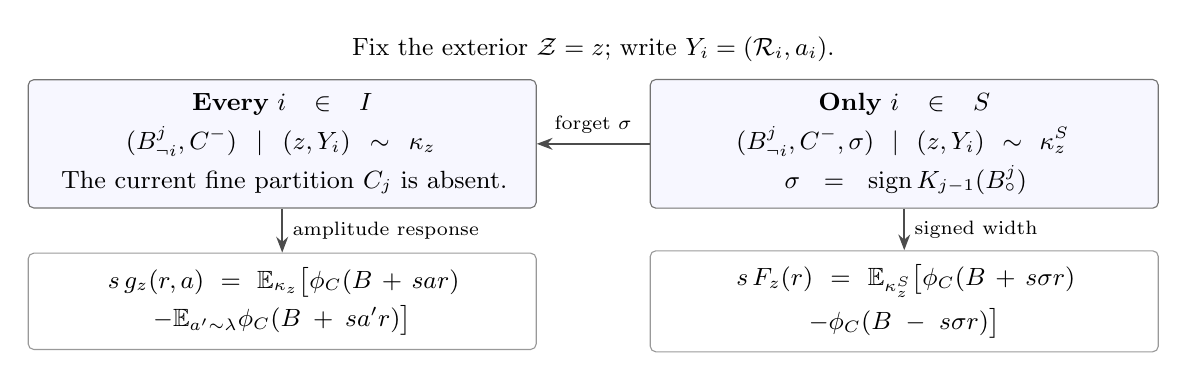
\begin{tikzpicture}[
  font=\small,
  kernel/.style={draw=black!55,fill=blue!3,rounded corners=2pt,
    align=center,text width=6.1cm,minimum height=1.35cm,inner sep=5pt},
  response/.style={draw=black!40,rounded corners=2pt,
    align=center,text width=6.1cm,minimum height=1.2cm,inner sep=5pt},
  map/.style={-{Stealth[length=2mm]},draw=black!70,thick}
]
\node[align=center] at (0,1.2)
  {Fix the exterior $\cZ=z$; write $Y_i=(\cR_i,a_i)$.};
\node[kernel] (ordinary) at (-3.95,0) {
  \textbf{Every $i\in I$}\\[3pt]
  $(B^j_{\neg i},C^-)\mid(z,Y_i)\sim\kappa_z$\\[3pt]
  The current fine partition $C_j$ is absent.
};
\node[kernel] (extended) at (3.95,0) {
  \textbf{Only $i\in S$}\\[3pt]
  $(B^j_{\neg i},C^-,\sigma)\mid(z,Y_i)\sim\kappa_z^S$\\[3pt]
  $\sigma=\operatorname{sign}K_{j-1}(B_\circ^j)$
};
\draw[map] (extended.west) -- node[above,font=\scriptsize]
  {forget $\sigma$} (ordinary.east);
\node[response] (amplitude) at (-3.95,-2.0) {
  $s\,g_z(r,a)=\E_{\kappa_z}\big[\phi_C(B+sar)$\\[3pt]
  $-\E_{a'\sim\lambda}\phi_C(B+sa'r)\big]$
};
\node[response] (width) at (3.95,-2.0) {
  $s\,F_z(r)=\E_{\kappa_z^S}\big[\phi_C(B+s\sigma r)$\\[3pt]
  $-\phi_C(B-s\sigma r)\big]$
};
\draw[map] (ordinary.south) -- node[right,font=\scriptsize]
  {amplitude response} (amplitude.north);
\draw[map] (extended.south) -- node[right,font=\scriptsize]
  {signed width} (width.north);
\end{tikzpicture}
\caption{The common coarse backgrounds, conditional on $\cZ=z$.
The displayed laws do not depend on $Y_i$; their index ranges differ.
Deleting the whole subbatch $S$ in $B_\circ^j$ makes the reference
sign independent of each tested $Y_i$, conditional on $z$, while
allowing dependence on the remaining background. The $(B,C)$ marginal
of $\kappa_z^S$ is $\kappa_z$, so the amplitude response can also be
averaged over the extended kernel. Here $C=C^-$, $\phi_C$ uses only
preceding smoothing, and the fresh predicate and amplitudes are
independent of the background conditional on $z$.}
\label{fig:conditional-kernels}
\end{figure}

\subsection{Forcing a slot and rebuilding the fine state}

Fix a mode $m$ and an index $i\in S$. Let $\cH_i$ contain $z$, $X$,
every current primary pair $Y_k$, and all current trials $T_k$ except
$T_i$. In particular it retains $Y_i$, whose original question list
still enters the fine partition when its summand is replaced.
The preceding partitions, $B_\circ^j$, and $\sigma$ are
$\cH_i$-measurable. The event
\[
 E_i=\{T_i\text{ is replacement in mode }m,
                  \ \tau_i=\sigma,\ \chi_i=+1\}
\]
has the exact conditional probability
\begin{equation}\label{eq:match-probability}
 \Prob(E_i\mid\cH_i)=\frac\alpha{2L2^J}=\beta.
\end{equation}
The number of formal parent cells is deterministic; empty cells and
colliding labels have not reduced $J$. Conditional on $E_i,\cH_i$, the
path data have their original mode law and $u$ is independent uniform.

Let $\Gamma(\cH_i,T_i)$ construct the entire stage-$j$ state, including
the score and the fine partition rebuilt from all unchanged primary
question lists and the trial's new path question list. For every
nonnegative measurable full-state function $Q_0$, the forced experiment
preserves the ordinary marginal law of $\cH_i$ and satisfies
\begin{equation}\label{eq:full-state-forcing}
 \E_{\rm forced}[Q_0(\Gamma)\mid\cH_i]
 =\E_{\rm actual}
       [Q_0(\Gamma)\ind_{E_i}/\beta\mid\cH_i].
\end{equation}
This is just conditional expectation under the event in
Equation~\ref{eq:match-probability}; it applies because the event
constrains only the mode, descriptor, and sign. It also holds for
integrable signed functions by subtraction. One may include independent
numerical noises in $\Gamma$, or integrate them in $h_j$ first.

In particular the identity permits $Q_0$ to depend on the new $C_j$,
its fine gradient, marks, and all current questions. There is no
conditioning on $C_j$ in Equation~\ref{eq:match-probability}: that
partition is an output of $\Gamma$. Deleting the whole subbatch in
$B_\circ^j$ ensures that the reference sign stays fixed as $T_i$ is
redrawn. It is essential here that we do not retain the old trial's fine
partition after replacing its path data.

Apply Equation~\ref{eq:full-state-forcing} for each $i\in S$, then
average. On the resulting single actual state there is one common
$C_j$, one $K_j$, and one $\sigma$. Put
\[
 d_z=|K_{j,z}|-\sigma_{\operatorname{par}(z)}K_{j,z},\qquad
 f_m=\operatorname{avg}_{i\in S}\ind_{E_i}.
\]
Then
\begin{equation}\label{eq:match-defect-transfer}
 \operatorname{avg}_{i\in S}\E_{\rm forced}\sum_zd_z
 =\E_{\rm actual}\sum_zd_z\frac{f_m}\beta
 \le2\E\sum_zd_z+\frac2\beta\E\sum_{z\text{ marked}}|K_{j,z}|
 \le4\Delta\nu.
\end{equation}
Indeed all descriptor counts are tested, so the count for the realized
$\sigma$ is among them. On an unmarked cell $f_m\le2\beta$;
everywhere $f_m\le1$ and $0\le d_z\le2|K_{j,z}|$. This is a pointwise
empirical inequality. It does not presume any independence of a
gradient and its match indicators. Goodness and the marked-gradient
budget pay for its last two terms. In particular the unmarked defect
is not multiplied by the reciprocal match probability.

For a vertical mode, retain the hit in the empirical fraction:
$f_{m,z}^{\rm hit}=\operatorname{avg}_{i\in S}\ind_{E_i}r_i^{\rm path}(z)$.
The same calculation, now conditional on $\cZ$, gives
\begin{equation}\label{eq:match-hit-transfer}
 \operatorname{avg}_{i\in S}\E_{\rm forced}
             \left[\sum_z|K_{j,z}|r_i^{\rm path}(z)\,\middle|\,\cZ\right]
 \le2p_{\rm law}\E[|K_j|_1\mid\cZ]
       +\beta^{-1}\E\left[\sum_{z\text{ marked}}|K_{j,z}|\,
                                                 \middle|\,\cZ\right].
\end{equation}
This uses the hit-match marking rule on each unmarked cell and the
bound $f_{m,z}^{\rm hit}\le1$ elsewhere.

\subsection{Endpoint conversion and path inequalities}

In the forced experiment use $\tau=\sigma$ and $\chi=+1$.
Compared with an independent uniform descriptor, this adaptive choice
is dominated by the factor $2^J$: conditional on the remaining variables,
the latter gives that descriptor probability $2^{-J}$. The fine state
is rebuilt in both experiments by the same rule. Thus
Equation~\ref{eq:forced-endpoint-bound} implies, for either endpoint,
\begin{equation}\label{eq:adaptive-endpoint-bound}
 \operatorname{avg}_{i\in S}\E_{\rm forced}
 \frac{|h_j(B^j_{\neg i}+sD^\pm)
                      -h_{j-1}(B^j_{\neg i}+sD^\pm)|}{s}
 \le\Delta\nu.
\end{equation}
The background and the sign use none of the forced slot's fresh path
data. This domination therefore changes only the descriptor choice.

For fixed path questions, mode, descriptor, and amplitude data, the
rebuilt fine partition is fixed as $u$ varies. Along
\[
 B(u)=B^j_{\neg i}+s[(1-u)D^-+uD^+]
\]
ordinary differentiation gives
\begin{equation}\label{eq:path-derivative}
 \frac1s\frac{\dd}{\dd u}h_j(B(u))
   =\sum_zK_{j,z}(B(u))(D^+(z)-D^-(z)).
\end{equation}
Each slope is $\sigma_{\operatorname{par}(z)}w_z$ with
$0\le w_z\le2$. Its negative part is bounded, conservatively, by
$2\sum_zd_z(B(u))$: if $\sigma K\ge0$ the coordinate contributes
no negative part, whereas if $\sigma K<0$, then
$-w_z\sigma K\le2(-\sigma K)\le2d_z$.
Integrating in $u$ and using Equation~\ref{eq:full-state-forcing}
identifies the uniform-time law with the actual gradient law in
Equation~\ref{eq:match-defect-transfer}. Converting the two endpoints
with Equation~\ref{eq:adaptive-endpoint-bound} proves, for every mode,
\begin{equation}\label{eq:oriented-path-bound}
 \operatorname{avg}_{i\in S}\E_{\rm forced}
 \left(\frac{h_{j-1}(B^j_{\neg i}+sD^-)
               -h_{j-1}(B^j_{\neg i}+sD^+)}s\right)_+
 \le10\Delta\nu.
\end{equation}
Here eight units pay for fine negative variation and two for the
endpoints. The estimates are uniform in the number of slots, cells,
and descriptors.

For a vertical mode, the absolute slope in
Equation~\ref{eq:path-derivative} is at most
$2\sum_z|K_{j,z}|r(z)$. Equation~\ref{eq:match-hit-transfer}, together
with $\E[|K_j|_1\mid\cZ]\le v$, bounds its conditional expected
integral by $4p_{\rm law}v$ plus a nonnegative error whose expectation
is at most $2\Delta\nu$. The two conditional endpoint errors add at
most $2\Delta\nu$ in expectation. Conditional Jensen's inequality and
Equation~\ref{eq:coarse-width} therefore give a nonnegative function
$e_{\rm law}(\cZ)$ such that
\begin{equation}\label{eq:width-vertical}
 \E_{r\sim P_{\rm law}}|F_{\cZ}(r)|
 \le4p_{\rm law}v+e_{\rm law}(\cZ),\qquad
 \E e_{\rm law}\le4\Delta\nu.
\end{equation}
This statement also covers zero-probability laws: their expected
unmarked contribution is zero and no division by their honest
probability has been used.

For an ordered coupling $(r,r')$, write the difference of coarse widths
as the sum of the difference of their upper endpoints and the reversed
difference of their lower endpoints. The two corresponding menu entries
are $+\sigma r\to+\sigma r'$ and
$-\sigma r'\to-\sigma r$. The positive part of a sum is at most the
sum of positive parts. Applying conditional Jensen and
Equation~\ref{eq:oriented-path-bound} twice yields
\begin{equation}\label{eq:width-order}
 \E_{\cZ,r,r'}(F_{\cZ}(r)-F_{\cZ}(r'))_+\le20\Delta\nu.
\end{equation}
The same background kernel is used for both endpoints because fresh
comparison data are drawn independently after the background.

For the amplitude comparison, use the common extended kernel described
after Equation~\ref{eq:coarse-width}. At one realization abbreviate
\[
 H_a=\phi_C(B+sar),\qquad H_-=\phi_C(B-s\sigma r),\qquad
 H_+=\phi_C(B+s\sigma r).
\]
Let $a'$ be an independent fresh amplitude. For any four real numbers
of this form,
\begin{equation}\label{eq:amplitude-sandwich}
 |H_a-H_{a'}|\le H_+-H_-
   +\sum_{b\in(a,a')}
          [(H_--H_b)_++(H_b-H_+)_+].
\end{equation}
The sum counts both amplitudes, including when $a=a'$.
Indeed write
$H_a-H_{a'}=(H_a-H_+)+(H_+-H_-)+(H_--H_{a'})$ and bound the first
and last terms by their positive parts. Adding the other two nonnegative
terms gives the right side of Equation~\ref{eq:amplitude-sandwich}.
Repeating with $a,a'$ exchanged bounds the opposite signed difference
by the same expression, proving the absolute-value bound without any
ordering assumption on $H_-,H_+$.

Divide Equation~\ref{eq:amplitude-sandwich} by $s$ and average over
the background and $a'$ with $\cZ,r,a$ fixed. The absolute value of the
averaged left difference is $|g_{\cZ}(r,a)|$ by
Equation~\ref{eq:common-amplitude-kernel}; the width term averages to
$F_{\cZ}(r)$. The four positive-part errors are supplied by the two
amplitude modes, once for $a$ and once for $a'$. Integrating the iid
predicate and amplitude laws and applying
Equation~\ref{eq:oriented-path-bound} four times proves
\begin{equation}\label{eq:width-amplitude}
 \E_{\cZ,r,a}(|g_{\cZ}(r,a)|-F_{\cZ}(r))_+\le40\Delta\nu.
\end{equation}
Equations~\ref{eq:width-vertical}, \ref{eq:width-order}, and
\ref{eq:width-amplitude} have constants $4,20,40$ independent of all
later scales. In their proof the oriented-path constant was ten.

\subsection{Selecting an exterior and threshold}

Draw a threshold $\vartheta$ independently and uniformly from
$[\gamma/4,\gamma/2]$. For each exterior $(\cZ,\vartheta)$ define
the common Boolean response on actual predicates
\[
 W(r)=\ind_{\{F_{\cZ}(r)>\vartheta\}}.
\]
Equation~\ref{eq:good-stage-signal} concerns a uniform index in $I$;
Equation~\ref{eq:common-amplitude-kernel} makes its response exactly the
common $g_{\cZ}(r,a)$ under the independent iid conjunction and amplitude
laws. On $|g_{\cZ}(r,a)|\ge\gamma$ but
$F_{\cZ}(r)\le\gamma/2$, the positive part in
Equation~\ref{eq:width-amplitude} is at least $\gamma/2$. Consequently
the lost mass is at most $80\Delta\nu/\gamma$. By
Equation~\ref{eq:delta-choice},
\begin{equation}\label{eq:threshold-success}
 \E_{\cZ,\vartheta}
   [\ind_{\{v\le B_*\}}\Prob_{P_*^t}(W=1)]
 \ge b_*p\nu/2.
\end{equation}
Indeed $F>\gamma/2$ ensures success for every possible threshold, and
the event no longer depends on the auxiliary amplitude.

For every vertical law and each fixed exterior,
Equation~\ref{eq:width-vertical} and $\vartheta\ge\gamma/4$ give
\begin{equation}\label{eq:threshold-upper}
 \Prob_{\rm law}(W=1)
 \le \frac{16}{\gamma}p_{\rm law}v
                              +\frac4\gamma e_{\rm law}(\cZ).
\end{equation}
Each final term has expectation at most $16\Delta\nu/\gamma$.
For real numbers $u,u'$, the probability over this random threshold
that $\ind_{\{u>\vartheta\}}>\ind_{\{u'>\vartheta\}}$ is at most
$4(u-u')_+/\gamma$, since the relevant threshold interval has length
at most $(u-u')_+$. Thus Equation~\ref{eq:width-order} gives, for each
ordered law,
\begin{equation}\label{eq:threshold-order}
 \E_{\cZ,\vartheta}\Prob(W(r)>W(r')\mid\cZ,\vartheta)
 \le80\Delta\nu/\gamma.
\end{equation}

Let $e_{\rm tot}(\cZ,\vartheta)$ be the sum of all $V$ upper-error
terms in Equation~\ref{eq:threshold-upper} and all $Q$ conditional
violation probabilities in Equation~\ref{eq:threshold-order}. It is
nonnegative and
\begin{equation}\label{eq:total-exterior-error}
 \E e_{\rm tot}\le A_t\Delta\nu/\gamma.
\end{equation}
Discard exteriors for which $e_{\rm tot}>\eps v$. The iid law is among
the vertical laws, so Equation~\ref{eq:threshold-upper} bounds the
integrated iid success on this discarded set by
\[
 \left(\frac{16p}{\gamma\eps}+1\right)\E e_{\rm tot}
 \le b_*p\nu/4.
\]
This estimate is relative to $\nu$ and remains valid for arbitrarily
small positive cut variance. Equations~\ref{eq:threshold-success}
and~\ref{eq:total-exterior-error} leave at least $b_*p\nu/4$ integrated
success on exteriors satisfying $v\le B_*$ and
$e_{\rm tot}\le\eps v$. An exterior in this set with $v=0$ has zero
success by its iid upper bound. Moreover $\E v\le(T_0+1)\nu$ by
Equation~\ref{eq:U-mean}. Since
$b_0(T_0+1)=b_*/8$, there must be a remaining exterior with $v>0$ and
\[
 \Prob_{P_*^t}(W=1)\ge b_0vp.
\]
Otherwise its integrated success would be at most $b_*p\nu/8$.
At this same exterior, every error summand is at most $\eps v$.
Consequently every fixed type pattern and prescribed ordered law satisfy
\[
 \Prob_{\rm pat}(W=1)\le v(K_0p_{\rm pat}+\eps),\qquad
 \Prob(W(r)>W(r'))\le\eps v,
 \qquad 0<v\le B_0.
\]
This is exactly Lemma~\ref{lem:rare-event}, with a single response
depending only on the conjunction as a predicate. It produces the
valuation forbidden by Lemma~\ref{lem:event-obstruction} in a NO
instance. The contradiction proves the soundness assertion of
Theorem~\ref{thm:score-gap}.

\subsection{The interface for finite compilation}\label{subsec:score-compilation}

We record the effective structure of the construction, including its
dependence on input size. The primitive test samplers use fixed mixtures
of uniform choices from polynomial-size finite sets. They therefore have
polynomially enumerable discrete sample spaces with rational probabilities
of polynomial bit length and inverse-polynomial lower bounds on positive
seed probabilities. For fixed $T_0$, all choices in
Equation~\ref{eq:preconjunction-constants}, the conjunction length,
the path menu, $\Delta$, $M$, and then the sequential stage parameters
are constants. The upper bounds on the required integers and the
numerical precision can be arbitrarily large functions of $T_0$; none
depends on the instance size.

\begin{proposition}[Finite form structure]\label{prop:score-compilation}
The demand law and the raw comparison measures in
Theorem~\ref{thm:score-gap} have polynomially enumerable discrete seeds,
whose positive probabilities are bounded below by an inverse polynomial
in input size. For each seed, after finitely many fixed subdivisions of
numerical boxes, their conditional densities are nonnegative rational polynomials and the
score table entries are rational polynomials of bounded degree in a
fixed number of numerical variables. There are only finitely many
such numerical polynomial patterns, independent of input size.
The total raw comparison mass is finite and bounded by a constant.
For any fixed finite grid and deterministic entrywise rounding rule, every positive
rounded demand mass or comparison-pair mass has an inverse-polynomial
lower bound.
\end{proposition}

\begin{proof}
Each sampled predicate has bounded arity and a polynomially enumerable
presentation law. A conjunction, a comparison path, and each slot use
a fixed number of those samples. The number of slots, stage choices,
freeze subsets, formal descriptors, and resampling indicators is fixed.
Enumerating their products therefore takes a polynomial number of
steps. All discrete probabilities are rational, with polynomial bit
length: products involve only a fixed number of primitive probabilities
and fixed rational weights. The same observation preserves an
inverse-polynomial lower bound for each positive seed probability.
Descriptor interpretation and refining the
lists require fixed-size truth tables with positions named by the seed.
Equality of names and the values of the finite test tables can be
computed in polynomial time.

Separate the amplitude atom at zero from its uniform part. All remaining
variables are amplitudes, interpolation times, and noises in rational
intervals, together with the integration variables in the derivative
forms. Their joint densities are products of rational polynomial
densities. Absolute derivative weights become polynomial on the two
half intervals, and $-f'_{\xi_j}$ is already nonnegative on its
integration interval. No lookup-dependent descriptor occurs in any
measure. All forms are positive measures on these fixed rectangular
pieces.

Fix a seed and an assignment to its bounded list of queried positions.
Each predicate value is then zero or one, each descriptor value is a
fixed sign, and each mark is determined by the finite trial counts.
The scores are sums of rational multiples of amplitudes, times, products
of time and fresh amplitude, and noises, multiplied by these fixed
Boolean values. Hence every score entry is a polynomial of bounded
degree with rational coefficients. The possible local Boolean tables,
label-collision patterns, descriptor vectors, and mark sets all range
over fixed finite sets. The numerical coefficients $s_j,\xi_j$ and
all external form weights have already been fixed. Therefore the
polynomial patterns belong to a fixed finite family; actual bit names
only select where a table is evaluated. This also shows a uniform bound
on arity and range of every score.

Finally, each derivative integral has mass at most
$15/(8\xi_j)$ per differentiated coordinate, and there are finitely
many formal cells. Ordinary comparison measures have mass one before
their finite external weights. Summing over the fixed set of forms
gives a finite bound on total raw mass.

Fix now a finite grid and entrywise rounding rule. For one numerical pattern,
every possible rounded local table, or pair of tables, has mass equal
to the integral of its fixed polynomial density over a fixed region
of its numerical box. These regions depend only on the pattern and
the fixed rounding rule. There are finitely many patterns and rounded
tables, so the minimum of all their positive masses is a positive
constant. Renaming the queried positions or identifying collisions
does not add numerical patterns. Any positive global rounded mass has
at least one contributing discrete seed. Multiplying its
inverse-polynomial probability by this fixed positive minimum proves
the last assertion; identifying identical scores only adds masses.
This completes both the proposition and the remaining effective assertions of
Theorem~\ref{thm:score-gap}.
\end{proof}

The parameter order can now be read without circular dependencies:
$T_0$ fixes the resampling and signal constants; these fix
$e,B_*,\gamma,b_0,K_0,B_0$; the rare-event lemma fixes $t,\eps$;
then $\Delta$ fixes $M$; finally each stage fixes
$\alpha_j,m_j,n_j,s_j,\xi_j$ in that order. The path constants above
do not grow when any later scale is made smaller or any stage size
larger.

\section{Finite graphs with exactly uniform demands}\label{sec:finite-graph}

We now convert Theorem~\ref{thm:score-gap} into the graph promised in
Theorem~\ref{thm:main}.  The conversion must retain cuts of arbitrarily small
positive mass.  In particular, replacing the demand by an additive approximation
alone would be insufficient.  We keep a multiplicative upper bound on the
retained demand and attach every remaining vertex to that demand.

Fix an integer $C'>C$, and set
\[
 A_0=10^{12},\qquad \kappa=C'A_0,\qquad T_0=100\kappa.
\]
Apply Theorem~\ref{thm:score-gap} with this $T_0$.  Write $\mu$ for its demand
law, and $\cD$ for the sum of its raw comparison forms.  Thus, for a perfect
witness $x$, the total truth cost is at most $4$, and
\begin{equation}\label{eq:demand-tails-finite}
 \Prob\{B^0(x)\ge1/4\}\ge10^{-4},\qquad
 \Prob\{B^0(x)\le-1/4\}\ge10^{-4}.
\end{equation}
In a NO instance, every measurable binary lookup $h$ with
$\nu=\Var_\mu(h)>0$ satisfies $\cD(h)>T_0\nu$.
All arities, numerical parameters, and total raw comparison weights below
are constants depending on $C$ only.

\subsection{Canonical keys and rational integration}

Let $b$ be the number of bit names in the test system. After fixing all
parameters of the score construction, unroll each complete demand or
comparison experiment, including both endpoints. Count all primitive
query occurrences: retained, frozen, and future primary lists, resampled
copies, fresh and forced path lists, and all lists defining formal
partitions. Counting repetitions gives an effectively computable bound
$Q_*=Q_*(C)$ on the number of distinct queried bit names in any experiment.
Descriptors, cell indicators, translations, and numerical noises introduce
no names beyond those lists. The finite sampler templates and their
sample counts are fixed by $C$, so $Q_*$ is independent of input size.
Choose $k=Q_*+1$; here $k$ is solely the key-enumeration bound.
Choose a bounded rational interval containing the ranges of all score
functions in these experiments, and a fixed finite rational grid in that
interval. Rounding means nearest-grid-point rounding
with a fixed rule at ties.  A \emph{key} is a grid-valued function on the bit
cube, specified by its ordered list of essential bit names and its truth
table.  Equal functions have the same key; sampling presentations are not
part of a key.  Enumerate all such keys of arity at most $k$.  If the grid
has $g$ values, there are at most
\[
 \sum_{j=0}^k\binom bj g^{2^j}
\]
keys.  This is polynomial in the original instance size.

Write $R(B)$ for entrywise rounding of a score.  If the entrywise error is at
most $\delta$ and the total raw comparison weight is $W_0$, then for each
truth assignment
\[
 \abs{R(B)(x)-R(\widetilde B)(x)}
 \le \abs{B(x)-\widetilde B(x)}+2\delta.
\]
Take the fixed grid fine enough that $2\delta W_0\le1$ and $\delta<1/16$.
The total rounded truth cost is then at most $5$, and the two demand tails
remain strictly outside $[-1/8,1/8]$.

Every coloring of the keys extends to a measurable lookup on the scores:
apply $R$ and then the coloring.  The range can be truncated outside the
interval used by the experiments and the function defined arbitrarily on
any unused scores.  Measurability follows because each rounded table is
specified by finitely many polynomial inequalities in the numerical
parameters of each experiment.  Consequently the soundness assertion of
Theorem~\ref{thm:score-gap} applies to every key coloring.

Here and below, $\mu_i$ denotes the pushforward demand mass of key $i$.
For an unordered pair of distinct keys, let $c^0_{ij}$ be its total raw
comparison weight, adding both possible orderings.  Self-comparisons
contribute zero.  Thus
\begin{equation}\label{eq:raw-capacities}
 \cD(h)=\sum_{i<j}c^0_{ij}\abs{h_i-h_j}.
\end{equation}
The numbers $c^0_{ij}$ and $\mu_i$ need not be rational.  The next observation
gives the particular approximations we require without exact real integration.

\begin{lemma}[Rational compilation]\label{lem:rational-compilation}
In polynomial time one can compute nonnegative rational numbers $c_{ij}$
and $l_i$ such that
\begin{align}
 &c_{ij}\ge c^0_{ij},\qquad
   \sum_{i<j}(c_{ij}-c^0_{ij})\le1,\label{eq:capacity-upper}\\
 &0\le l_i\le\mu_i,\qquad L:=\sum_i l_i\ge1-10^{-6}.
   \label{eq:demand-lower}
\end{align}
Their binary encoding lengths are polynomial.  Every positive $l_i$ is at
least an inverse polynomial in the input size, with the polynomial depending
only on $C$.
\end{lemma}

\begin{proof}
Enumerate the discrete seeds in the demand and comparison experiments.
There are polynomially many seeds: the number of samples per experiment is
fixed, and every bit-test sampling space has polynomial size.  Their
probabilities are rational with polynomial encoding length, and every
positive discrete sampling probability is at least an inverse polynomial.

Conditional on a seed, the remaining numerical variables range over
rectangular boxes of fixed dimension.  Atoms and signs are separate discrete
choices.  The smoothing densities and comparison weights are polynomial
with rational coefficients on finitely many rectangular pieces; absolute
derivative weights are split at their changes of sign.  Each score-table
entry is a polynomial with fixed rational coefficients in these variables.
These assertions also hold for forced-slot comparisons, common-noise
comparisons, path interpolation, cell translation, and the formal cell sums:
all involve a fixed number of additions and products of the prescribed
amplitudes, marks, and shifts.  Only the local Boolean tables of the queried
predicates and their bit-name identifications enter these formulas.  Their
sizes are bounded, so, after forgetting the actual bit names, only a fixed
finite collection of numerical patterns occurs.  In particular, the
lookup-dependent reference sign used in the proof of soundness is not used
to define any comparison weight. The input-dependent rational seed
probabilities remain outside these conditional numerical integrals;
they do not enlarge the finite family of polynomial coefficients.

Subdivide each numerical box into rational boxes.  For every grid boundary
and every table entry, first check whether the polynomial entry is
identically equal to that boundary; if so, resolve the tie by the fixed
rounding rule.  Otherwise its equality set has Lebesgue measure zero.
Indeed, a nonzero polynomial in one variable has finitely many roots; in
higher dimension expand in the last variable, apply the induction
hypothesis to the simultaneous vanishing of its coefficients, and then
apply the one-variable assertion on the remaining fibers.  Integration
over fibers proves the claim.

Coefficient bounds on a bounded box give a rational Lipschitz bound for
every polynomial entry.  Comparing its value at a rational box corner
with this bound times the mesh identifies every box on which rounding
is determined.  Apart from the finitely many null boundary sets, each
point is eventually in such a box.  Since the weights are bounded, the
total weighted mass of unresolved boxes tends to zero.

On a resolved box integrate its polynomial weight term by term, obtaining
an exact rational mass.  For demand, discard unresolved boxes.  For
capacities, assign the full box mass to every table pair that could occur
there. One may conservatively use every grid-valued table on the queried
coordinates: each has at most $Q_*<k$ essential names and hence a key in
the enumerated universe. Their number is a constant. This gives an upper bound for
each pair mass.  Its excess is bounded by that constant times the weighted
unresolved mass.  Take the mesh fine enough that demand loses at most
$10^{-6}$ and capacity gains at most $1$ in total.  Because the numerical
patterns form a fixed finite collection, one fixed mesh works for every
seed and every input.  Equivalently, rational subdivision can continue
until the explicit unresolved-mass bounds meet these tolerances.  Averaging
these bounds with the seed probabilities gives the stated errors; the
errors are not summed without those probabilities. More explicitly, let
$U_{f,\omega,\ell}$ be the unresolved polynomial mass of rectangular
piece $\ell$ in comparison form $f$, conditional on seed $\omega$,
with its external form weight included. If $\pi_{f,\omega}$ is the seed
probability and $R_{f,\omega,\ell}$ bounds the number of candidate
unordered distinct key pairs, require
\[
 \sum_f\sum_\omega\pi_{f,\omega}
       \sum_\ell R_{f,\omega,\ell}U_{f,\omega,\ell}\le1.
\]
All formal-cell, derivative-coordinate, and rectangular pieces are
counted with their multiplicities. The analogous demand sum, with no
pair factor, must be at most $10^{-6}$. These are exact rational stopping
tests. A common mesh depth succeeds for every numerical pattern; an
input that stops earlier uses a depth no larger than that fixed bound.

At this fixed mesh, the positive retained conditional demand-box masses
belong to a fixed finite set of positive rational numbers. The same is
true over all mesh depths up to the fixed bound. Each therefore
has a positive constant lower bound.  A positive $l_i$ includes one of
these masses multiplied by a positive discrete seed probability, proving
the inverse-polynomial lower bound.  There are polynomially many seeds
and a constant number of boxes and table entries per seed.  Their rational
arithmetic, including the final sums, has polynomial bit complexity.
\end{proof}

Normalize the retained demand by $\widehat\mu_i=l_i/L$.  From
Equations~\eqref{eq:demand-lower} we have, for every key and every set $E$ of
keys,
\begin{equation}\label{eq:retained-demand}
 \widehat\mu_i\le2\mu_i,\qquad
 \widehat\mu(E)\ge\mu(E)-10^{-6}.
\end{equation}
For the second assertion use $\widehat\mu(E)\ge l(E)$ and
$\mu(E)-l(E)\le1-L$.

\subsection{Replication and auxiliary vertices}

Let $m$ be the number of keys, and choose an integer $K$ at least
$4\kappa m$ and at least the reciprocal of the smallest positive
$\widehat\mu_i$.  Lemma~\ref{lem:rational-compilation} permits $K$ of
polynomial magnitude.  Replace key $i$ by a cluster of
\[
 n_i=\begin{cases}
 \lceil K\widehat\mu_i\rceil,&\widehat\mu_i>0,\\
 1,&\widehat\mu_i=0
 \end{cases}
\]
vertices, designating one representative.  Put $N=\sum_i n_i$ and
$w_i=n_i/N$.  Since $K\le N\le K+m$, we obtain
\begin{equation}\label{eq:replication-weights}
 \frac12\widehat\mu_i\le w_i\le2\widehat\mu_i
 \quad(\widehat\mu_i>0),\qquad
 \alpha:=\sum_{\widehat\mu_i=0}w_i\le\frac1{4\kappa}.
\end{equation}
For the upper bound use $K\widehat\mu_i\ge1$; for the lower bound use
$K\ge m$.  Every key has a positive number of copies.

Place capacity $c_{ij}$ between representatives $i,j$.  Join every other
vertex in cluster $i$ to its representative by an edge of capacity
$2\kappa$.  Finally, if $\widehat\mu_i=0$ and $\widehat\mu_j>0$, add capacity
\[
 2\kappa w_i\widehat\mu_j
\]
between their representatives.  These last edges are the \emph{tethers}.
Add capacities when edges coincide, and set all diagonal capacities to
zero.  Give every unordered pair of distinct vertices demand exactly one.
The output threshold is the positive rational number
\begin{equation}\label{eq:final-threshold}
 a=\frac{A_0}{N^2}.
\end{equation}

\subsection{Completeness}

Suppose $x$ is a perfect witness.  For a common threshold
$\theta\in[-1/8,1/8]$, color key $i$ by
$h_i=\ind_{\{i(x)>\theta\}}$, and give its copies the same color.
The tails in Equation~\eqref{eq:demand-tails-finite}, their preservation by
rounding, and Equations~\eqref{eq:retained-demand}--\eqref{eq:replication-weights}
show that both sides of every such cut have counting mass at least
\[
 \tfrac12(10^{-4}-10^{-6})\ge\tau,\qquad
 \tau:=10^{-4}/4.
\]
Thus all these cuts are proper and nonempty.

Take $\theta$ uniformly in that interval.  For any two real values $u,v$,
the probability that the threshold separates them is at most $4\abs{u-v}$.
The expected raw rounded comparison capacity is consequently at most
$4\cdot5=20$.  The excess in Equation~\eqref{eq:capacity-upper} contributes
at most $1$, and the total tether capacity is
$2\kappa\alpha\le1/2$.  No coherence edge crosses.  In particular, the
expected cut capacity is at most $22$, so some threshold cut has capacity
at most $22$.  If its counting mass is $z$, then $z,1-z\ge\tau$ and
\[
 \frac{\operatorname{cap}(S,V\setminus S)}{|S|(N-|S|)}
 \le\frac{22}{N^2\tau^2}
 <\frac{A_0}{N^2}=a,
\]
because $A_0\tau^2=625>22$.

\subsection{Soundness}

Suppose the formula is unsatisfiable and a nonempty proper cut has ratio
at most $C'a$.  Let $z=|S|/N$ and let $T$ be its capacity.  Then
\begin{equation}\label{eq:putative-small-cut}
 T\le\kappa z(1-z)\le\kappa/4.
\end{equation}
A split cluster would cut an edge of capacity $2\kappa$, so every cluster
is monochromatic.  The cut therefore determines a binary coloring $h_i$
of the keys and hence a measurable lookup on scores.  Set
\[
 \nu=\Var_\mu(h),\qquad
 L_{\rm aux}=\sum_{\widehat\mu_i=0}w_i
                    \sum_j\widehat\mu_j\abs{h_i-h_j}.
\]
The tethers contribute exactly $2\kappa L_{\rm aux}$.

We claim
\begin{equation}\label{eq:variance-transfer}
 z(1-z)\le36\nu+L_{\rm aux}.
\end{equation}
To prove this, draw a key with distribution $w$.  Retain it if its
$\widehat\mu$ mass is positive, and otherwise replace it by an independent
$\widehat\mu$ draw.  The color changes with probability $L_{\rm aux}$.
The replacement distribution is
\[
 \rho_j=\ind_{\{\widehat\mu_j>0\}}w_j+\alpha\widehat\mu_j
 \le3\widehat\mu_j\le6\mu_j.
\]
Apply this coupling independently to two $w$ draws.  Their original
disagreement probability is $2z(1-z)$; their replacement disagreement
probability is at most $36\cdot2\nu$ by the product domination
$\rho\otimes\rho\le36\mu\otimes\mu$.  A union bound for the two possible
color changes proves Equation~\eqref{eq:variance-transfer}.

Combining the claim with Equation~\eqref{eq:putative-small-cut} and the
tether lower bound gives
\[
 T\le36\kappa\nu+\kappa L_{\rm aux}
 \le36\kappa\nu+T/2,
 \qquad\text{hence}\qquad T\le72\kappa\nu.
\]
Moreover $\nu>0$: otherwise these inequalities give $T=0$, then
$L_{\rm aux}=0$, and Equation~\eqref{eq:variance-transfer} gives
$z(1-z)=0$, contrary to the cut being proper and nonempty.
By Equations~\eqref{eq:raw-capacities}--\eqref{eq:capacity-upper},
\[
 \cD(h)\le T\le72\kappa\nu<T_0\nu.
\]
This contradicts Theorem~\ref{thm:score-gap}.  Every nonempty proper cut in
a NO instance therefore has ratio strictly greater than $C'a$.

\subsection{Complexity and conclusion}

Every enumeration above is polynomial in the original formula size; its
exponent may depend on $C$.  The rational compilation has polynomial bit
complexity, the replication creates polynomially many vertices, and all
capacities and the threshold have polynomial binary encodings.  The
construction does not inspect a satisfying assignment or a candidate cut.
It is therefore a polynomial-time reduction with
\[
 \text{YES}:\ \Phi(G)\le a,
 \qquad
 \text{NO}:\ \Phi(G)>C'a.
\]
A factor-$C$ approximation outputs a cut of ratio at most $Ca<C'a$ in the
YES case, whereas every cut has ratio greater than $C'a$ in the NO case.
Testing the output ratio against the rational number $C'a$ decides the
original satisfiability instance.  This proves Theorem~\ref{thm:main}.

\bibliographystyle{plain}
\bibliography{references}
\end{document}
